\documentclass[]{article}



\usepackage{graphicx,forloop,caption,subcaption,float,hyperref,arrayjob,listings,color,booktabs,mathtools}
\usepackage{pdfpages}
\usepackage[margin=1.2in]{geometry}
\usepackage{amsmath}
\usepackage{multirow}
%vhdl code
\definecolor{dkgreen}{rgb}{0,0.6,0}
\definecolor{gray}{rgb}{0.5,0.5,0.5}
\definecolor{mauve}{rgb}{0.58,0,0.82}

\DeclareMathOperator*{\argmin}{\arg\!\min}
\newcommand{\rom}[1]{\uppercase\expandafter{\romannumeral#1}}

\lstset{frame=tb,
  language=VHDL,
  aboveskip=3mm,
  belowskip=3mm,
  showstringspaces=false,
  columns=flexible,
  basicstyle={\small\ttfamily},
  numbers=none,
  numberstyle=\tiny\color{gray},
  keywordstyle=\color{blue},
  commentstyle=\color{dkgreen},
  stringstyle=\color{mauve},
  breaklines=true,
  breakatwhitespace=true
  tabsize=3
}

%matlab code
\lstset{frame=tb,
  language=Matlab,
  aboveskip=3mm,
  belowskip=3mm,
  showstringspaces=false,
  columns=flexible,
  basicstyle={\small\ttfamily},
  numbers=none,
  numberstyle=\tiny\color{gray},
  keywordstyle=\color{blue},
  commentstyle=\color{dkgreen},
  stringstyle=\color{mauve},
  breaklines=true,
  breakatwhitespace=true
  tabsize=3
}


% Title Page
\title{UCLA\\EE230B\\Digital Communication Design Project\\Step 2 Report}
\author{Alican Salor 404271991 \\  \href{mailto:alicansalor@ucla.edu}{alicansalor@ucla.edu} \\ \\
Darren Reis 804359840 \\
\href{mailto:darrer.r.reis@gmail.com}{darren.r.reis@gmail.com} }


\begin{document}
\maketitle

\newpage
\tableofcontents

\newpage


\section{System Setup}
\label{sec:setup}
The system is as shown in Figure below:

\begin{figure}[H]
\centering
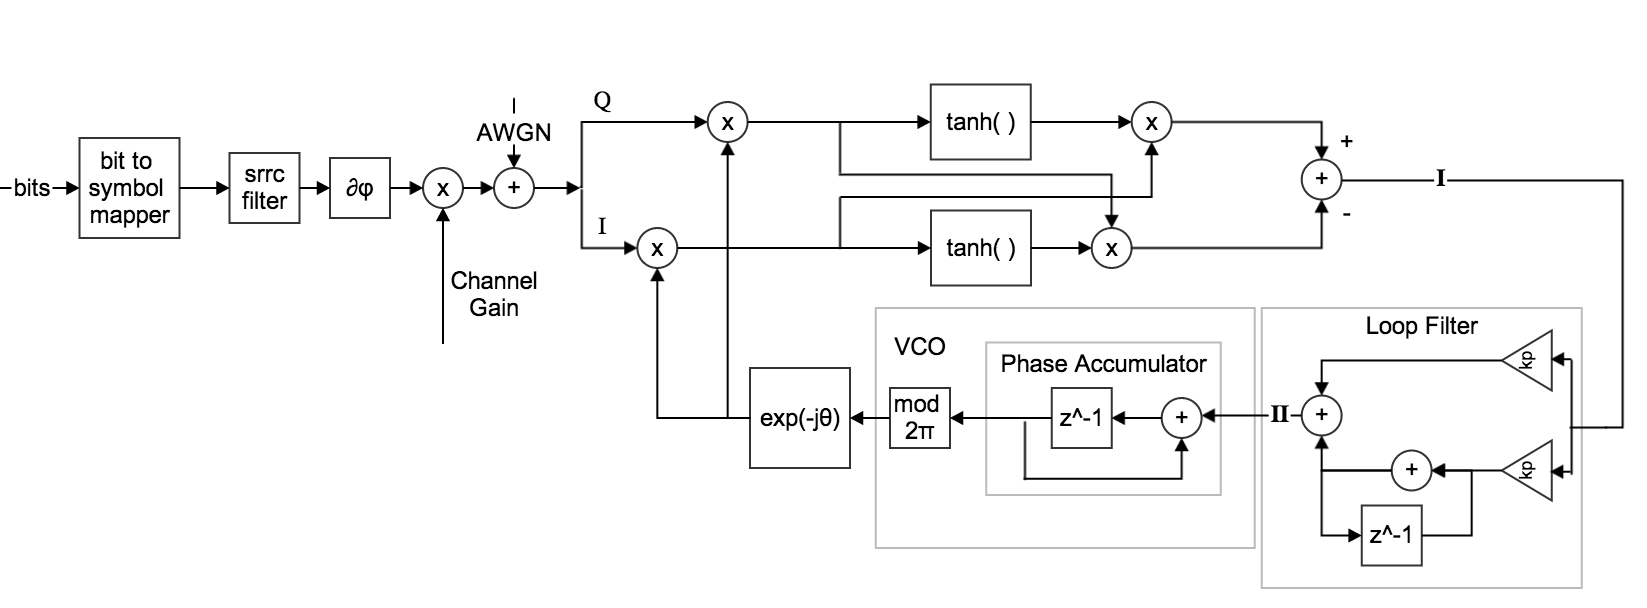
\includegraphics[width=\textwidth]{costas.png}
\caption{Diagram of the Costas loop used to handle error\label{fig:costas}}
\end{figure}

\begin{figure}[H]
\centering
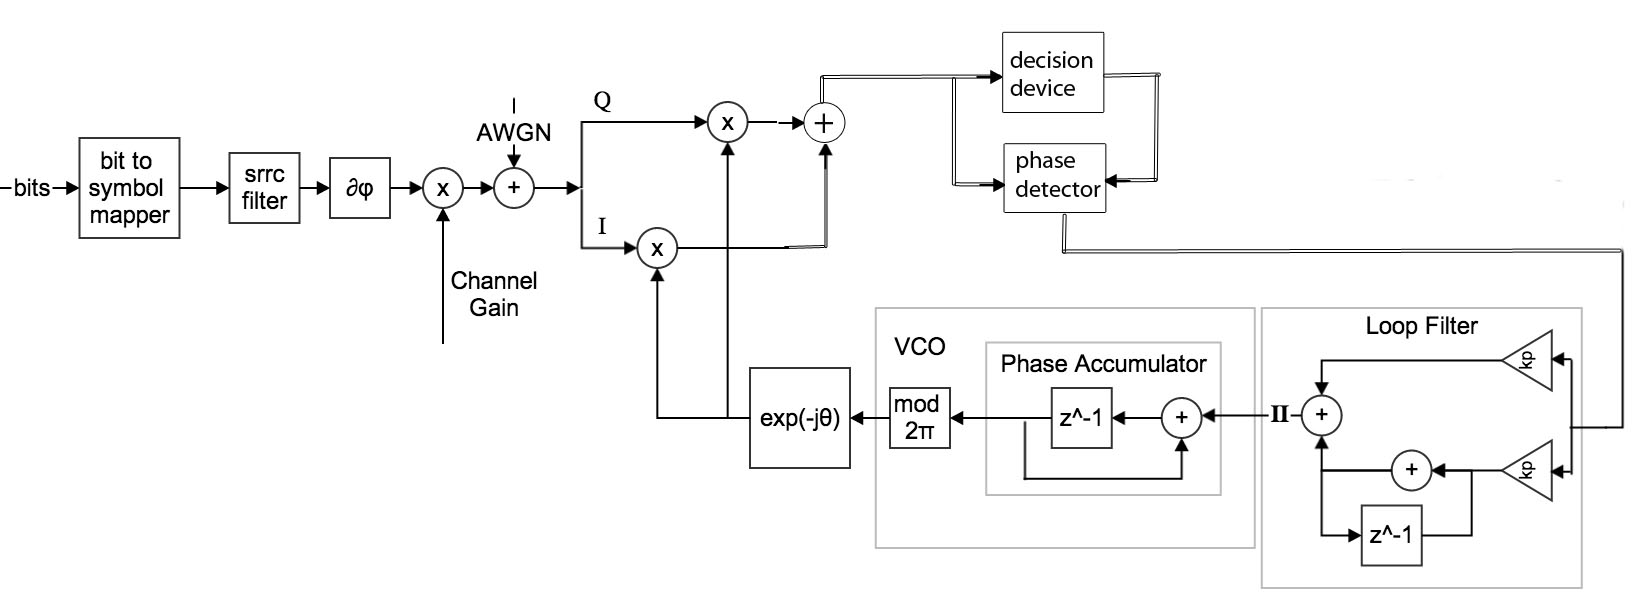
\includegraphics[width=\textwidth]{ddr_diagram.jpg}
\caption{Diagram of the Decision Directed Recovery loop used to handle error}
\end{figure}


To handle the noncoherent error introduced into the system, feedback loops were installed.  As from before, the $\delta\phi$ block represents a block that introduces phase or frequency offset on the carrier.  To combat this, the error is estimated and then fed into a feedback loop filter to track it out.  This is accomplished first via a Costas loop, as in Figure~\ref{fig:costas}.  Note that unlike in previous simulations of the system, this analysis required sample-wise operations instead of signal-wise operations.  That is, to maintain causality, the samples were analyzed one by one so that future samples could not influence present values.
\section{Costas Loop Theory}
\label{sec:costas}
The phase and frequency offset error, under QPSK, can be handled by a Costas loop.  The technique first creates an estimate of the phase error by creating a metric for it.  The error is then sent through a closed feedback loop.  This structure can track out the zero order and first order phase errors. 
\subsection{Phase Metric}
\label{sec:phaseMetric} 
In a Costas loop, the I and Q component of the received signal are both sent through a $\tanh\left(\cdot\right)$ block in order to discern their sign.  This works because for $k>>1$, $\text{sign}\left(x\right) \approx \tanh \left(x\right)$.  These $\pm1$ are multiplied by the opposite component signal.  The I component is then subtracted from the Q component, creating a phase error metric [\ref{eq:costas}].  This is labeled in Figure~\ref{fig:costas} as \rom{1}.  Section~\ref{sec:scurves} discusses how this estimate changes with different phase error.  Now with an error metric, we have an input to run into a loop filter. 

  \begin{align}
  \label{eq:costas}
  S_{\mathcal{l}} &= \left[I\left(t\right)\sin\left(\phi_e\right)+Q\left(t\right)\cos\left(\phi_e\right)\right]\text{sign}\left(I\left(t\right)\cos\left(\phi_e\right)- Q\left(t\right)\sin\left(\phi_e\right)\right)\nonumber \\
  &\qquad {} - \left[I\left(t\right)\cos\left(\phi_e\right)-Q\left(t\right)\sin\left(\phi_e\right)\right]\text{sign}\left(I\left(t\right)\sin\left(\phi_e\right)+Q\left(t\right)\cos\left(\phi_e\right)\right)
  \end{align}
  
\subsection{Feedback}
In control theory, the plant is the open loop system.  When there is steady state error in the open loop system, feedback, or `closing the loop' can track out the error.  From the plots in Step 2, we realize our situation is just this case of steady state error.  Depending on the order of the system, this error can become unbounded and damning.  Feedback can track or bound this error by `closing the loop' if the open loop system Type is 0.  \footnote{Recall, a system is of Type N when there N poles at the s-plane origin.}  Here, the steady state error can be held to a certain level by introducing integration in the feedback line of the loop.  For us, this is true when we talk about phase error: we can send a step input phase error into a Voltage Controlled Oscillator and watch the error converge to a constant level.  This is done in Section~\ref{sec:BLAH}. 
\begin{align}
\label{eq:vco}
\phi_{\text{out}} &= \int \! k_{VCO}V_{in} \mathrm{d}t
\end{align}
A VCO is a device with output oscillation which is varied by the voltage level of the input.  The transfer function, relating the input to the output, for this block is shown in Equation~\ref{eq:vco}. The integral action can eliminate phase error, as we see in Figure~\ref{fig:BLAH}.  To implement a VCO in simulation, a phase accumulator does the integration   action and then, to keep the result in the correct domain, the result is put through a modulo $2\pi$ block.   
When the plant is of higher Type than 0, as with a frequency offset, the steady state error can grow unbounded.  To deal with this scenario, another block is inserted in the feedback line.  An additional integrator increases the order of the closed loop system to allow bounding of higher type systems.  Notice in Figure~\ref{fig:costas}, the loop filter is Proportional-Integral.  With two integrators in the feedback path, Type 1 systems, or those with ramp inputs, can be bounded to a constant steady state error level.  Because frequency can be thought of as first order phase [\ref{eq:phaseFreq}], we track out the frequency error in Section

\begin{align}
\label{eq:phaseFreq}
\phi &= \int \! 2\pi f \mathrm{d}t 
\end{align}


\newpage
\section{Step 3 Results}
\subsection{QPSK with Costas Loop}

\subsubsection{S-Curve of Phase Detector}
\begin{figure}[H]
\centering
\hspace*{-2cm}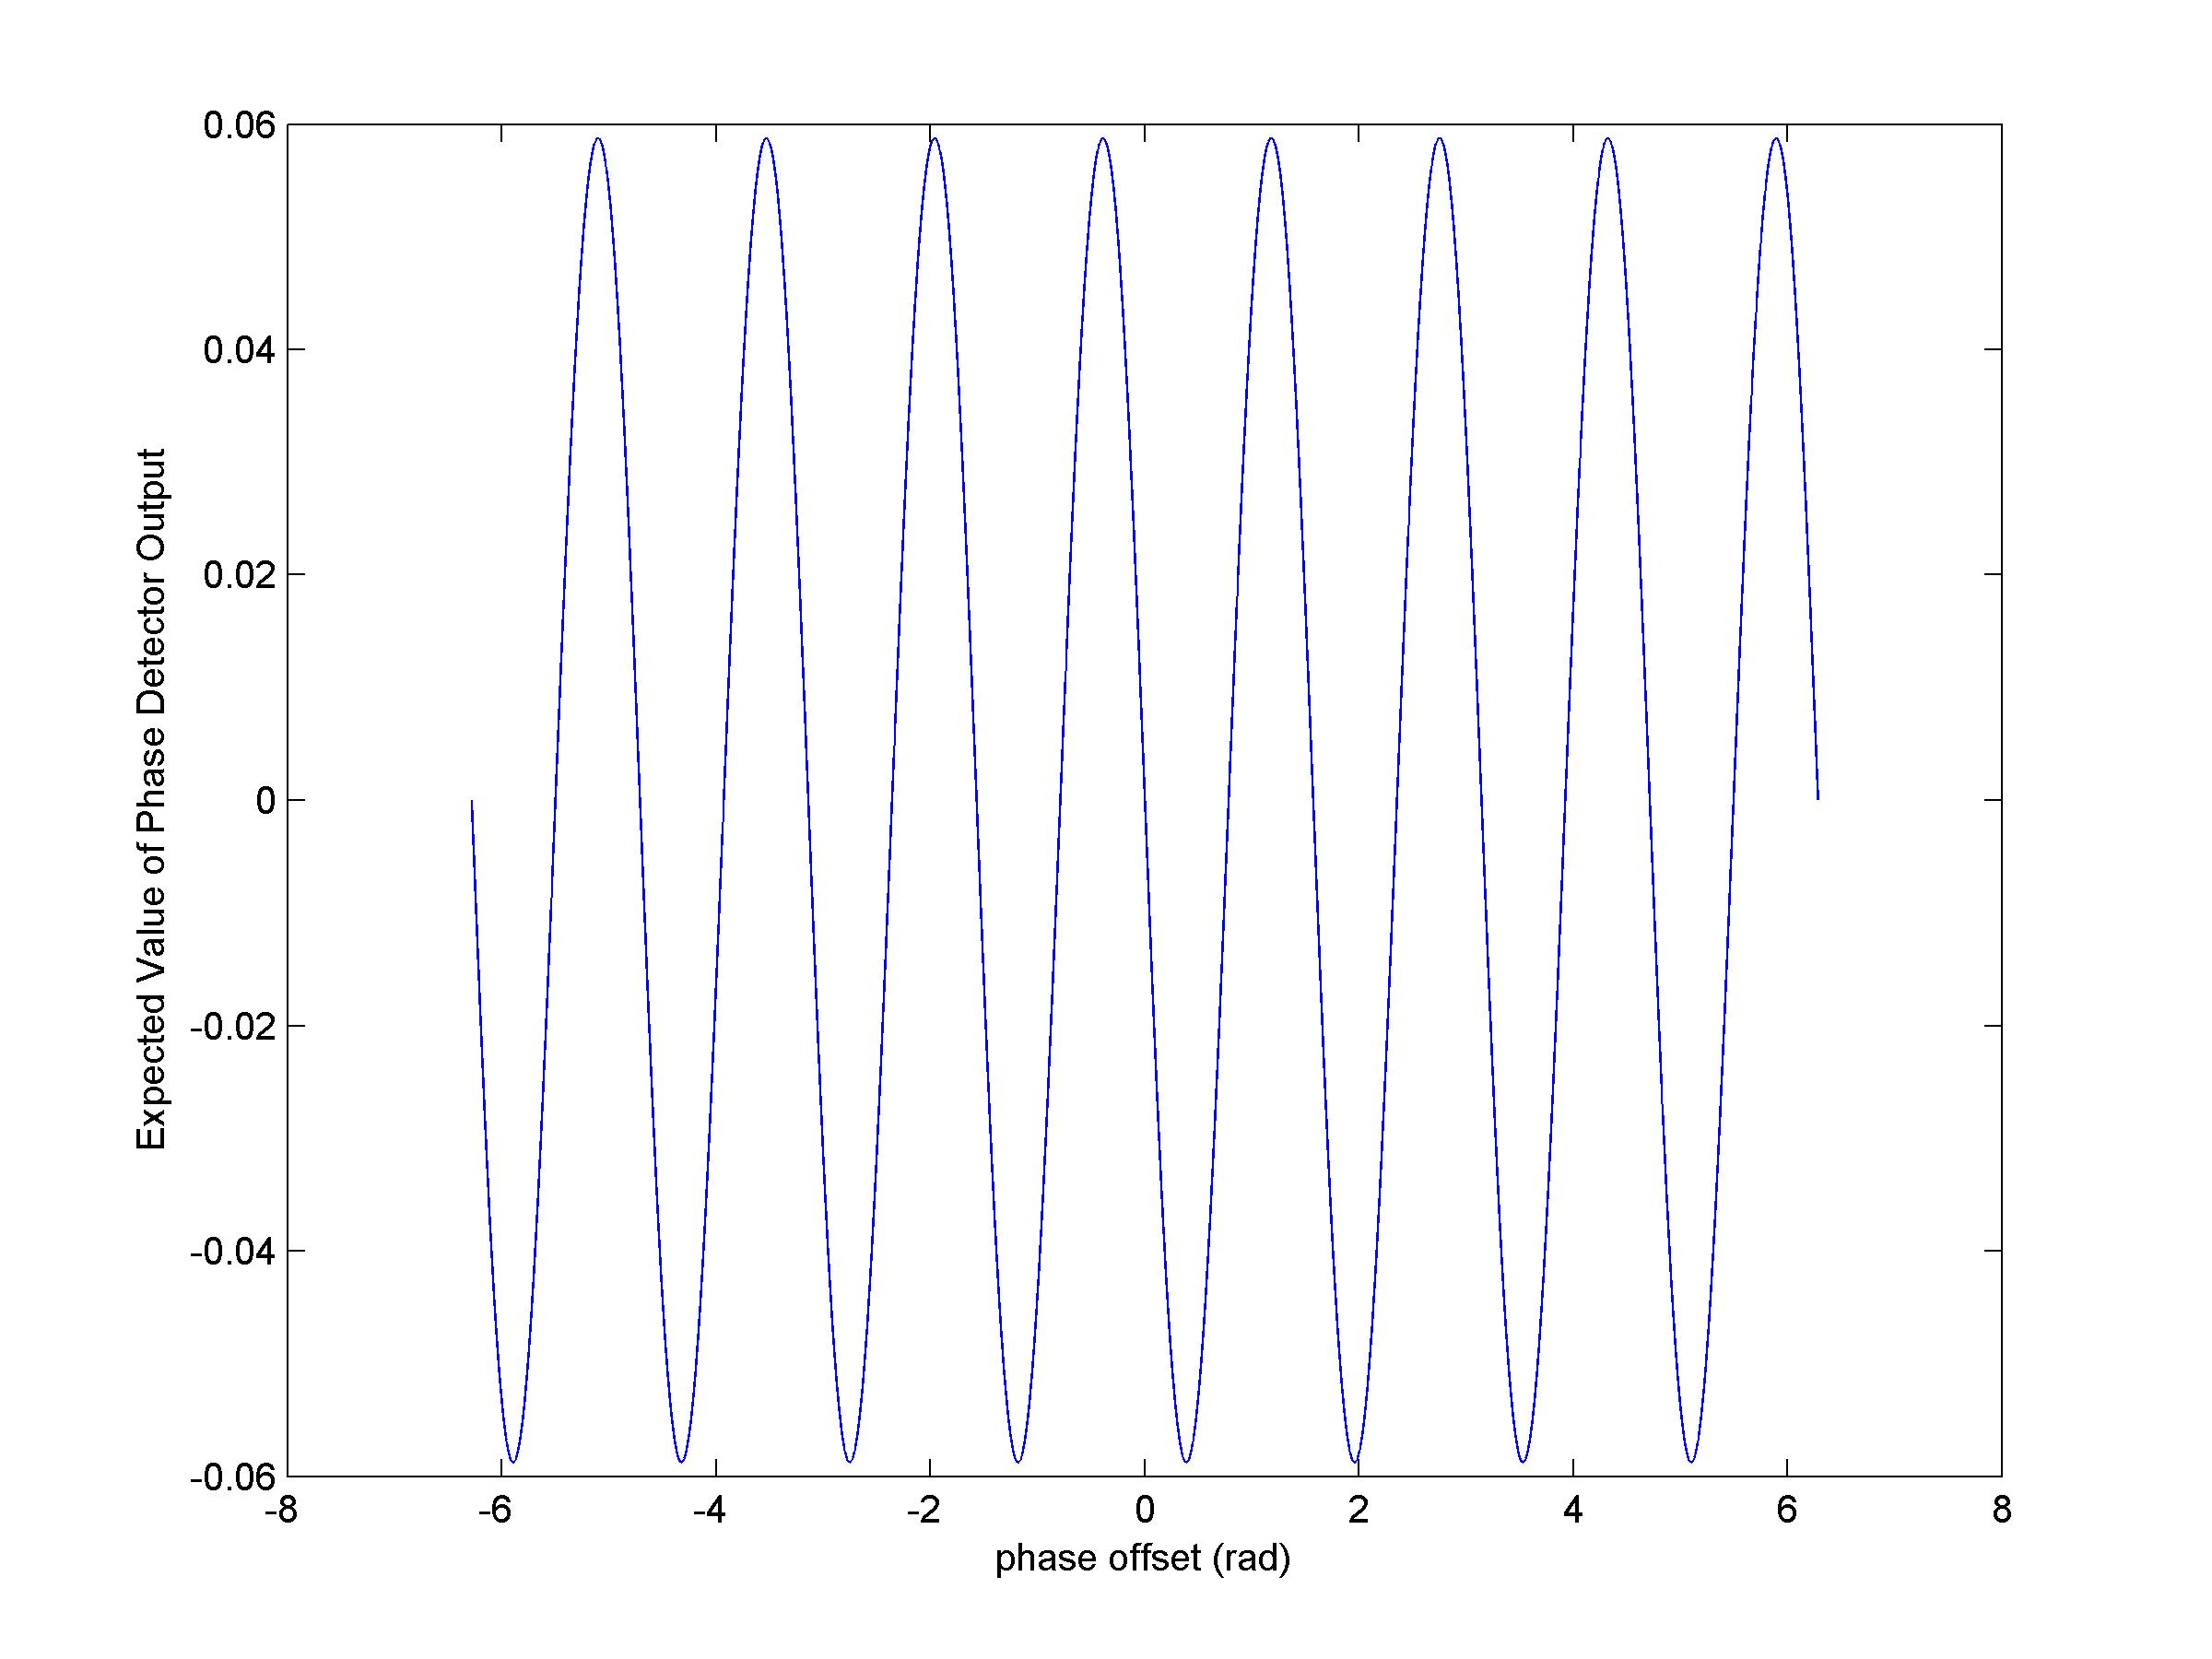
\includegraphics[width=0.5\textwidth]{qpScurvepo_costas.jpg}
\caption{}
\end{figure}
\subsubsection{S-Curve of Carrier Detector}
\begin{figure}[H]
\centering
\hspace*{-2cm}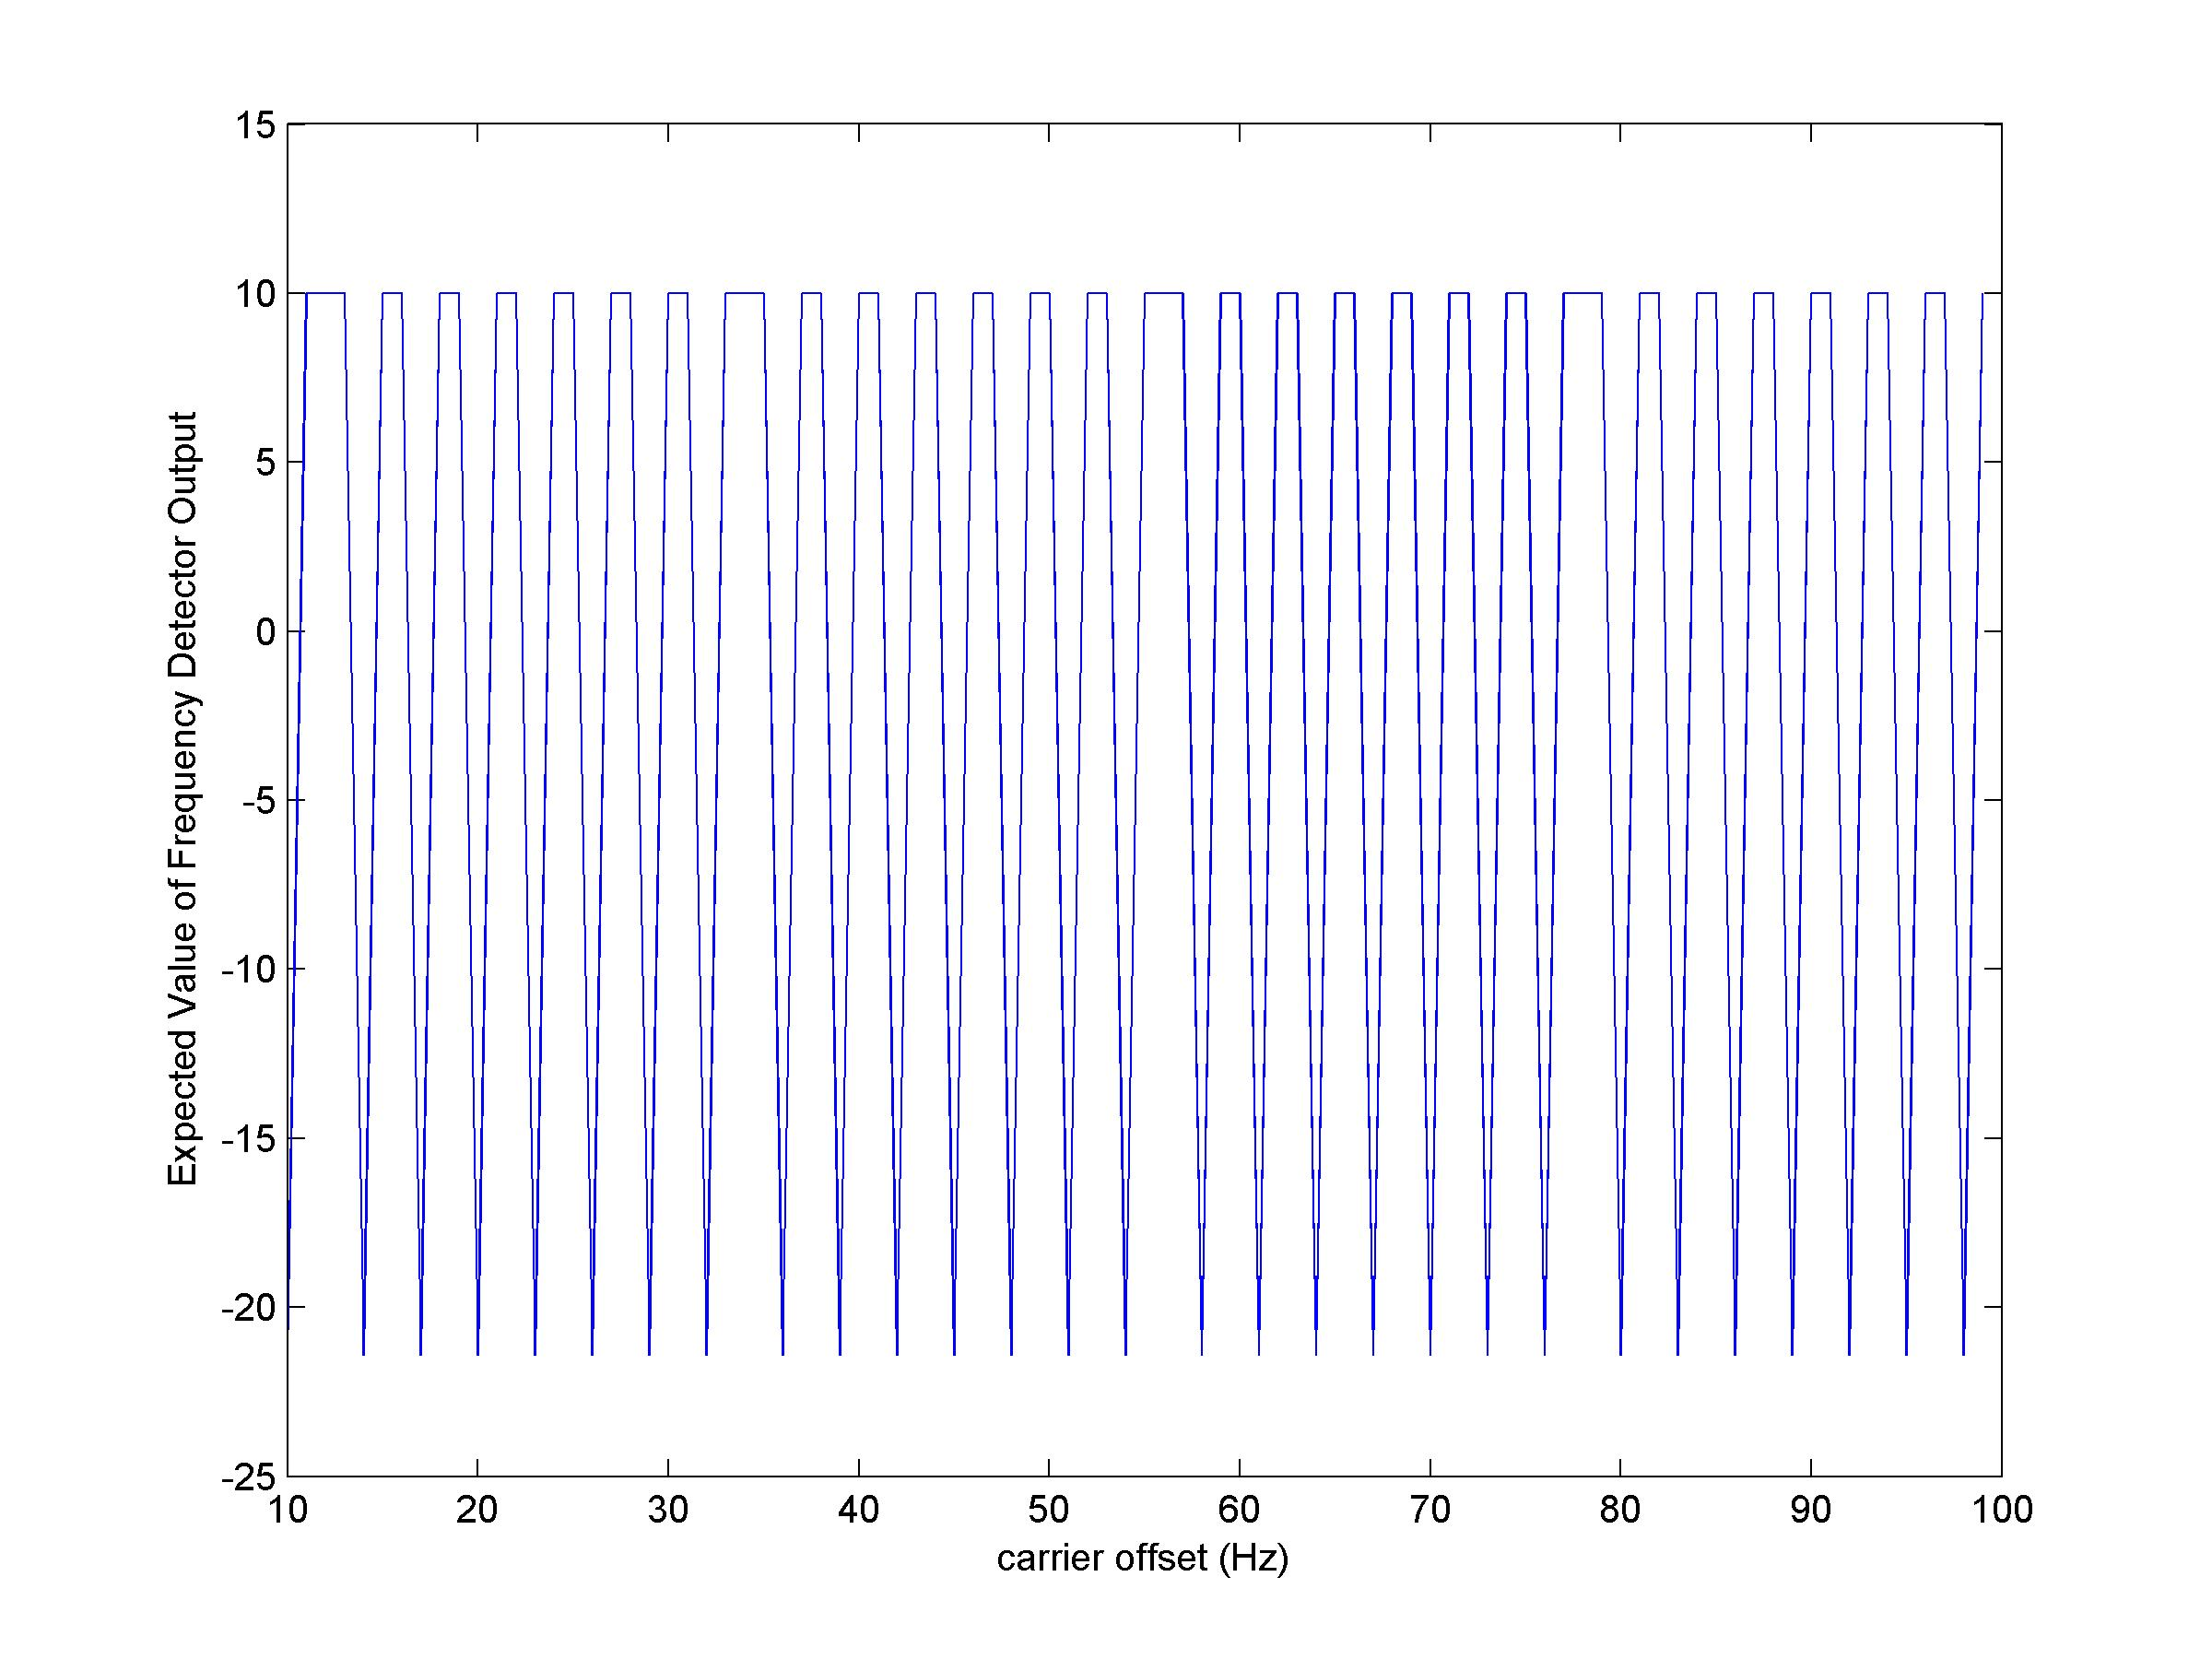
\includegraphics[width=0.5\textwidth]{qpScurvefo.jpg}
\caption{}
\end{figure}
\subsubsection{Transience of Phase Recovery}
\begin{figure}[H]
\centering
\hspace*{-2cm}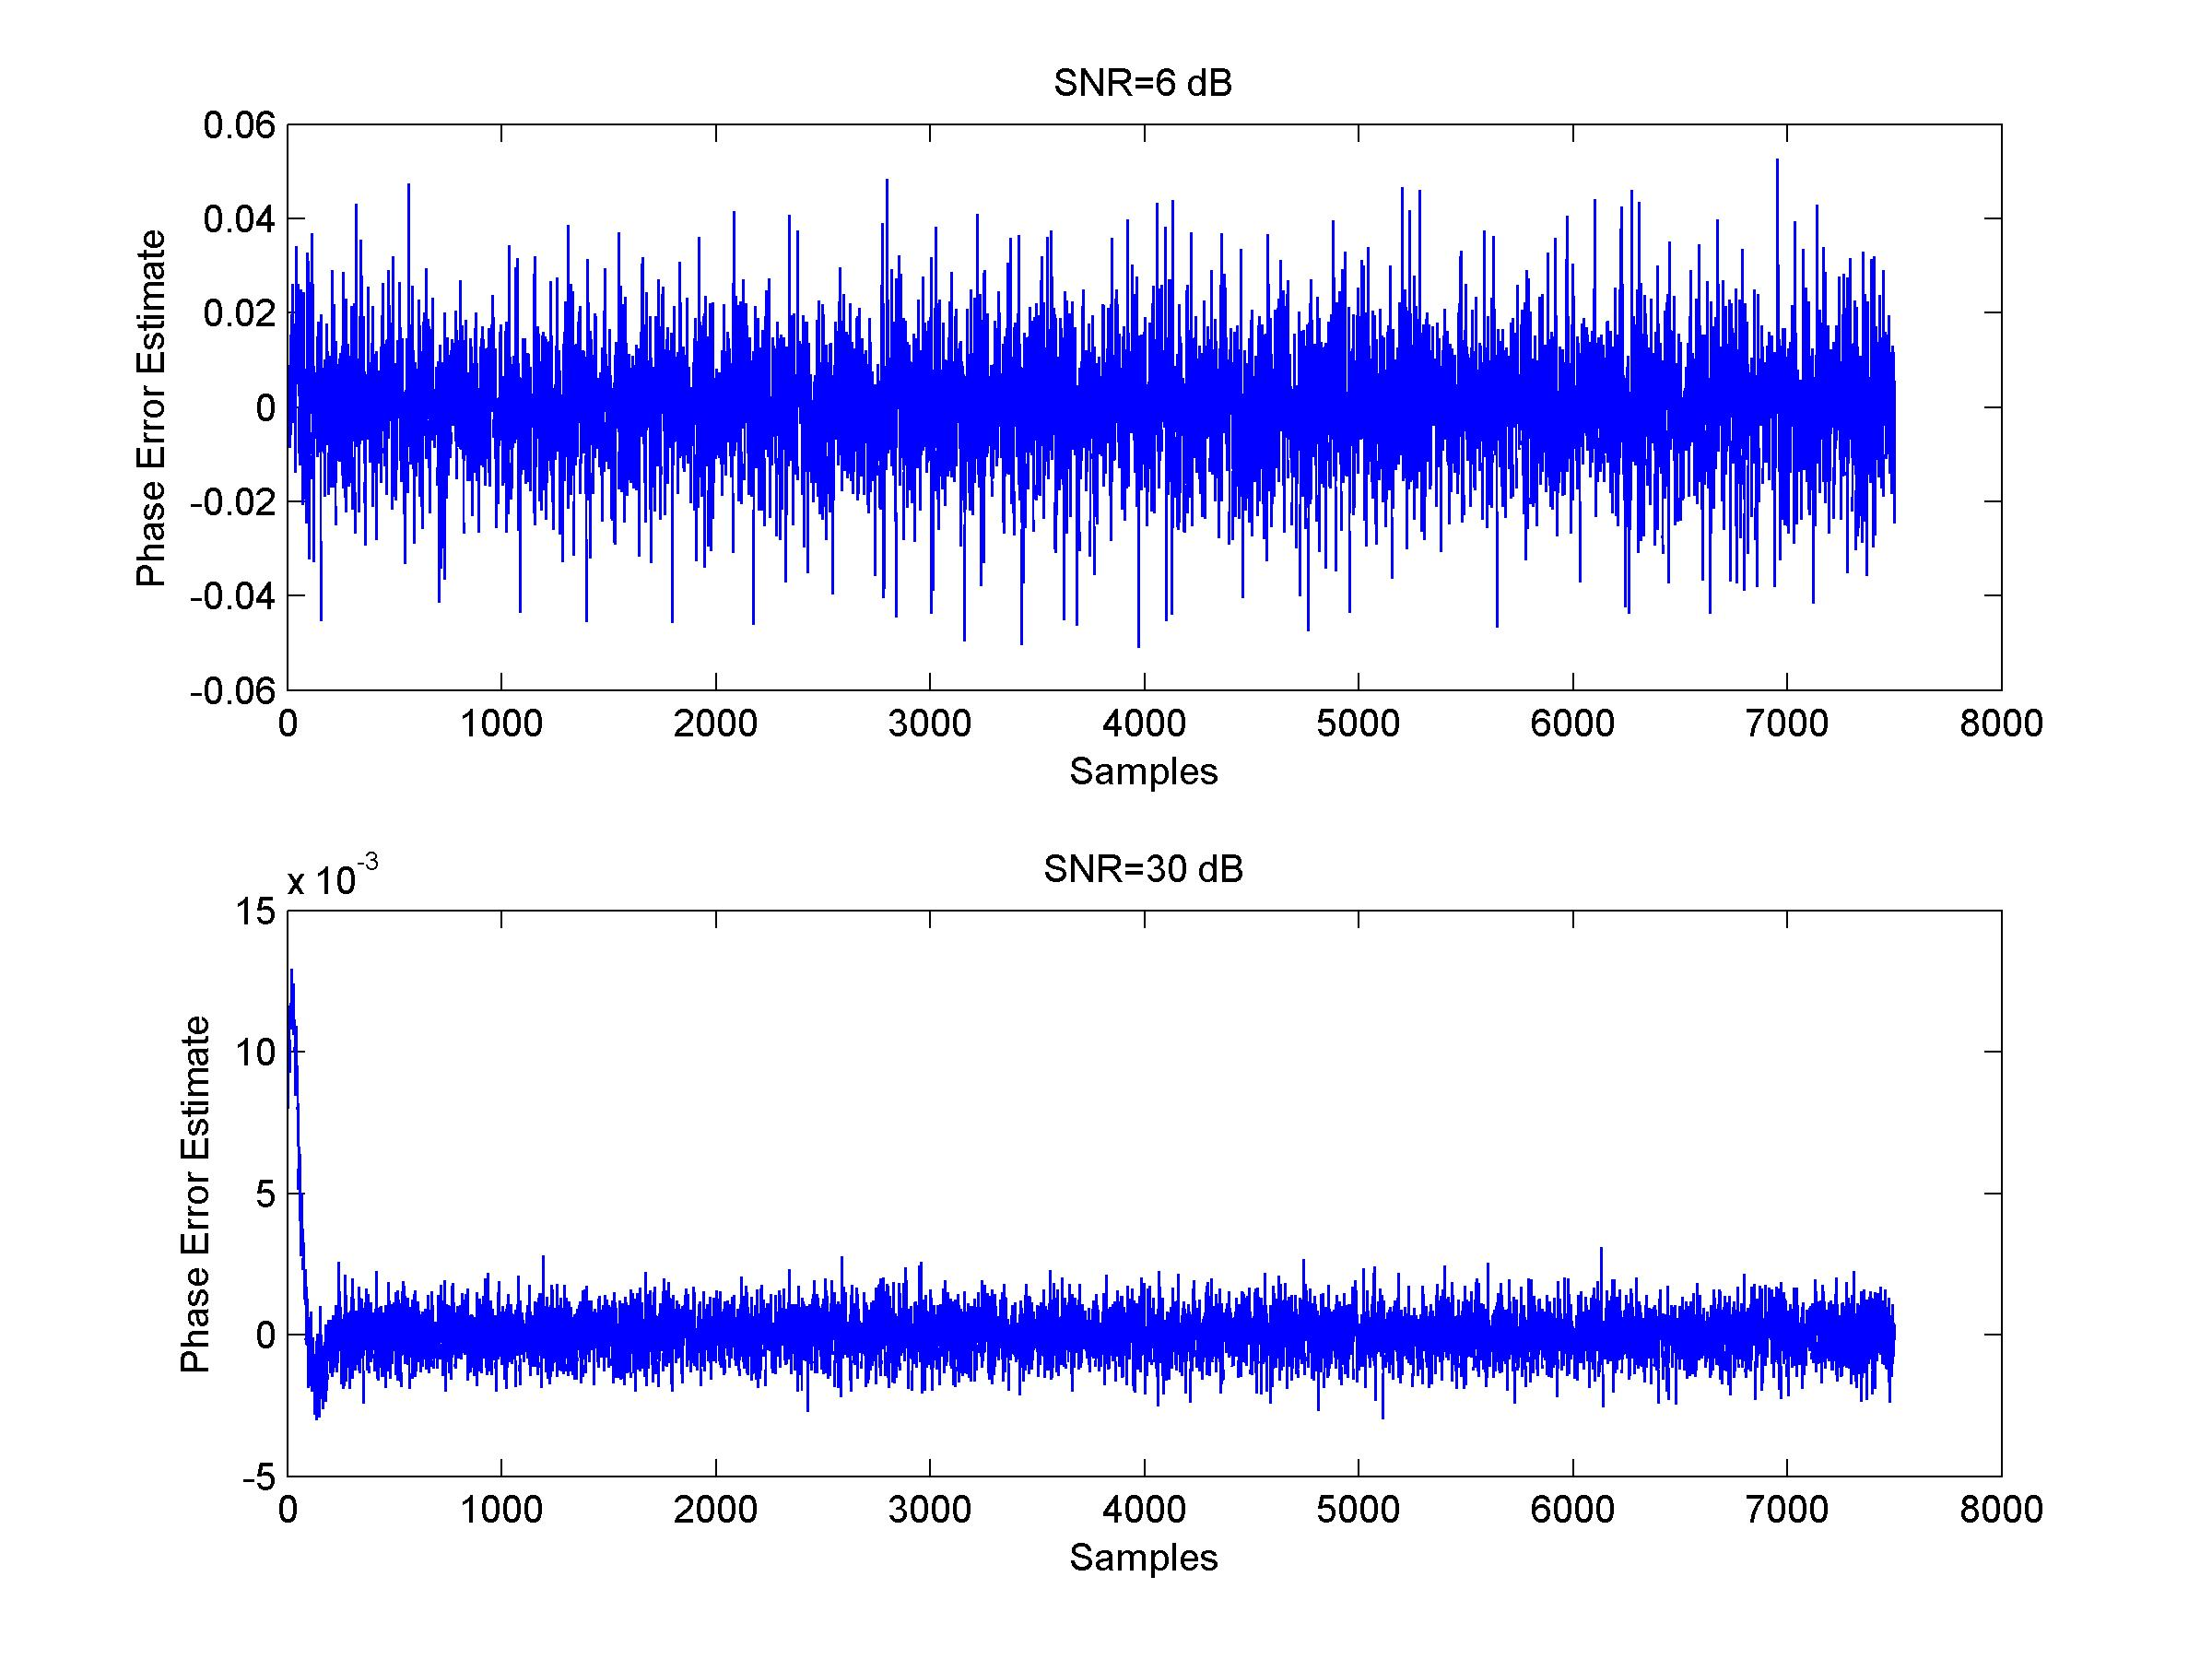
\includegraphics[width=0.5\textwidth]{qpLoopFilterpo_costas1.jpg}
\caption{}
\end{figure}

\subsubsection{Transience of Carrier Recovery}
\begin{figure}[H]
\centering
\hspace*{-2cm}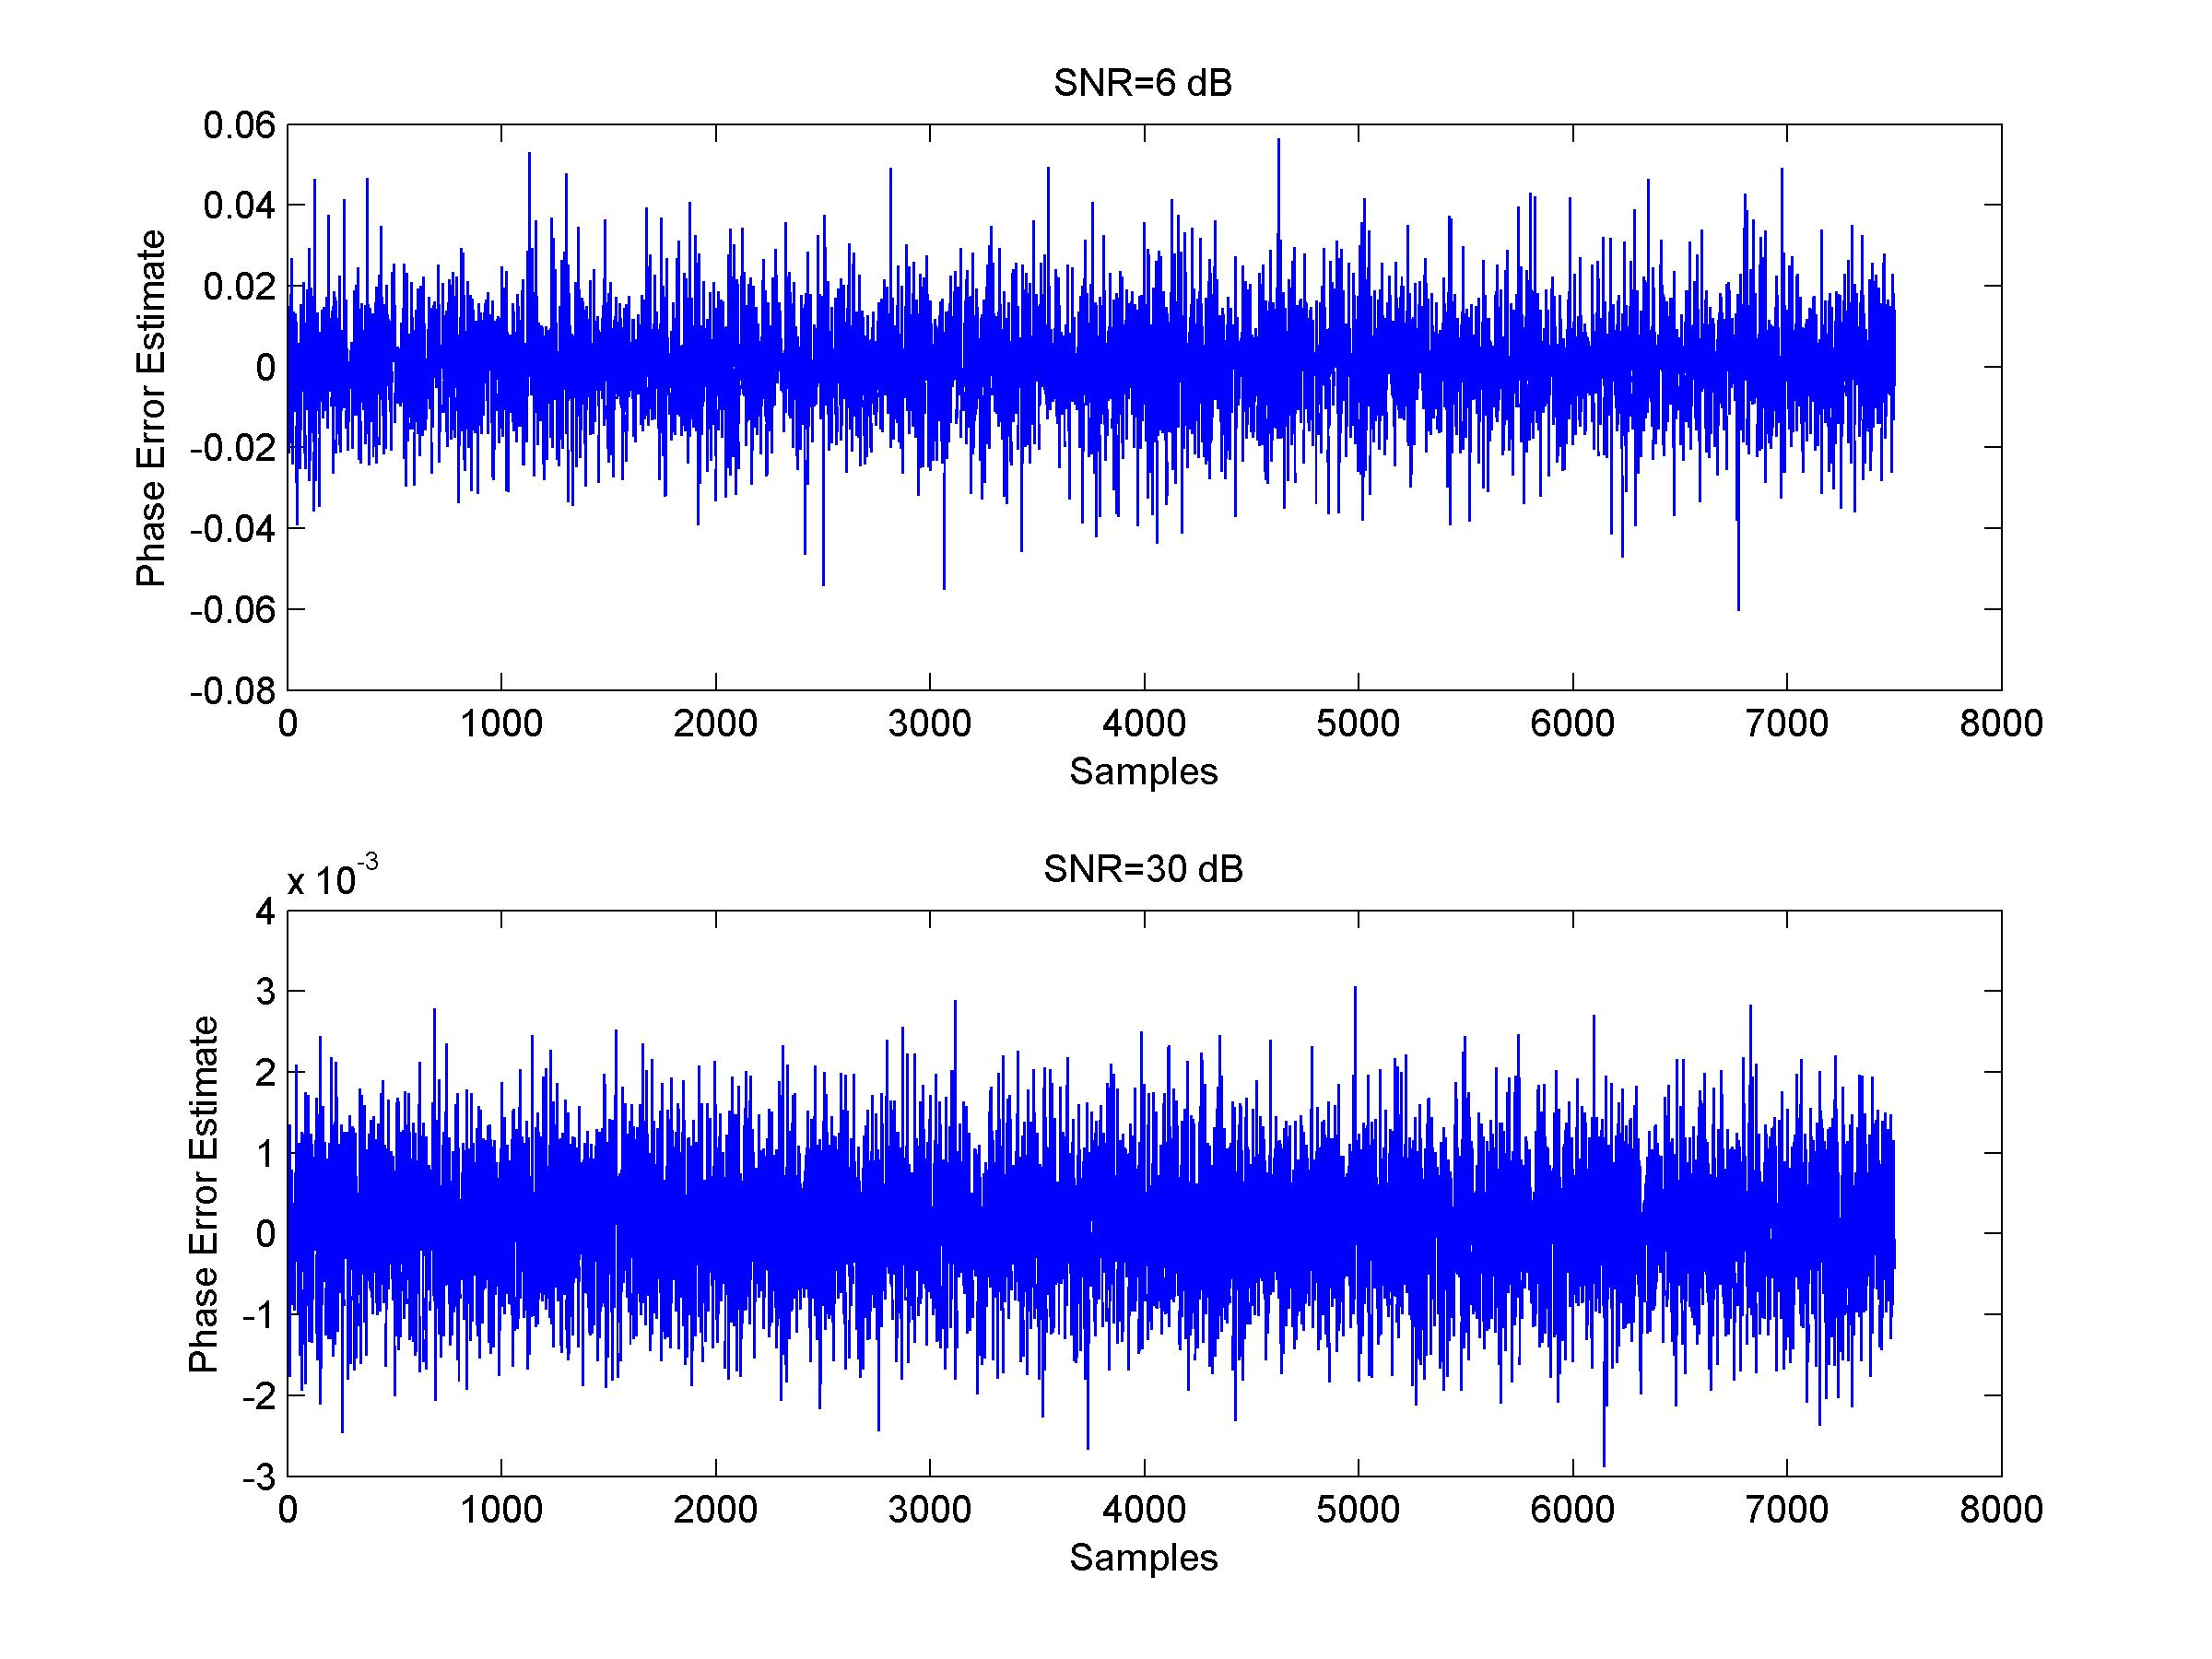
\includegraphics[width=0.5\textwidth]{qpLoopFilterfo_costas1.jpg}
\caption{}
\end{figure}

\begin{figure}[H]
\centering
\hspace*{-2cm}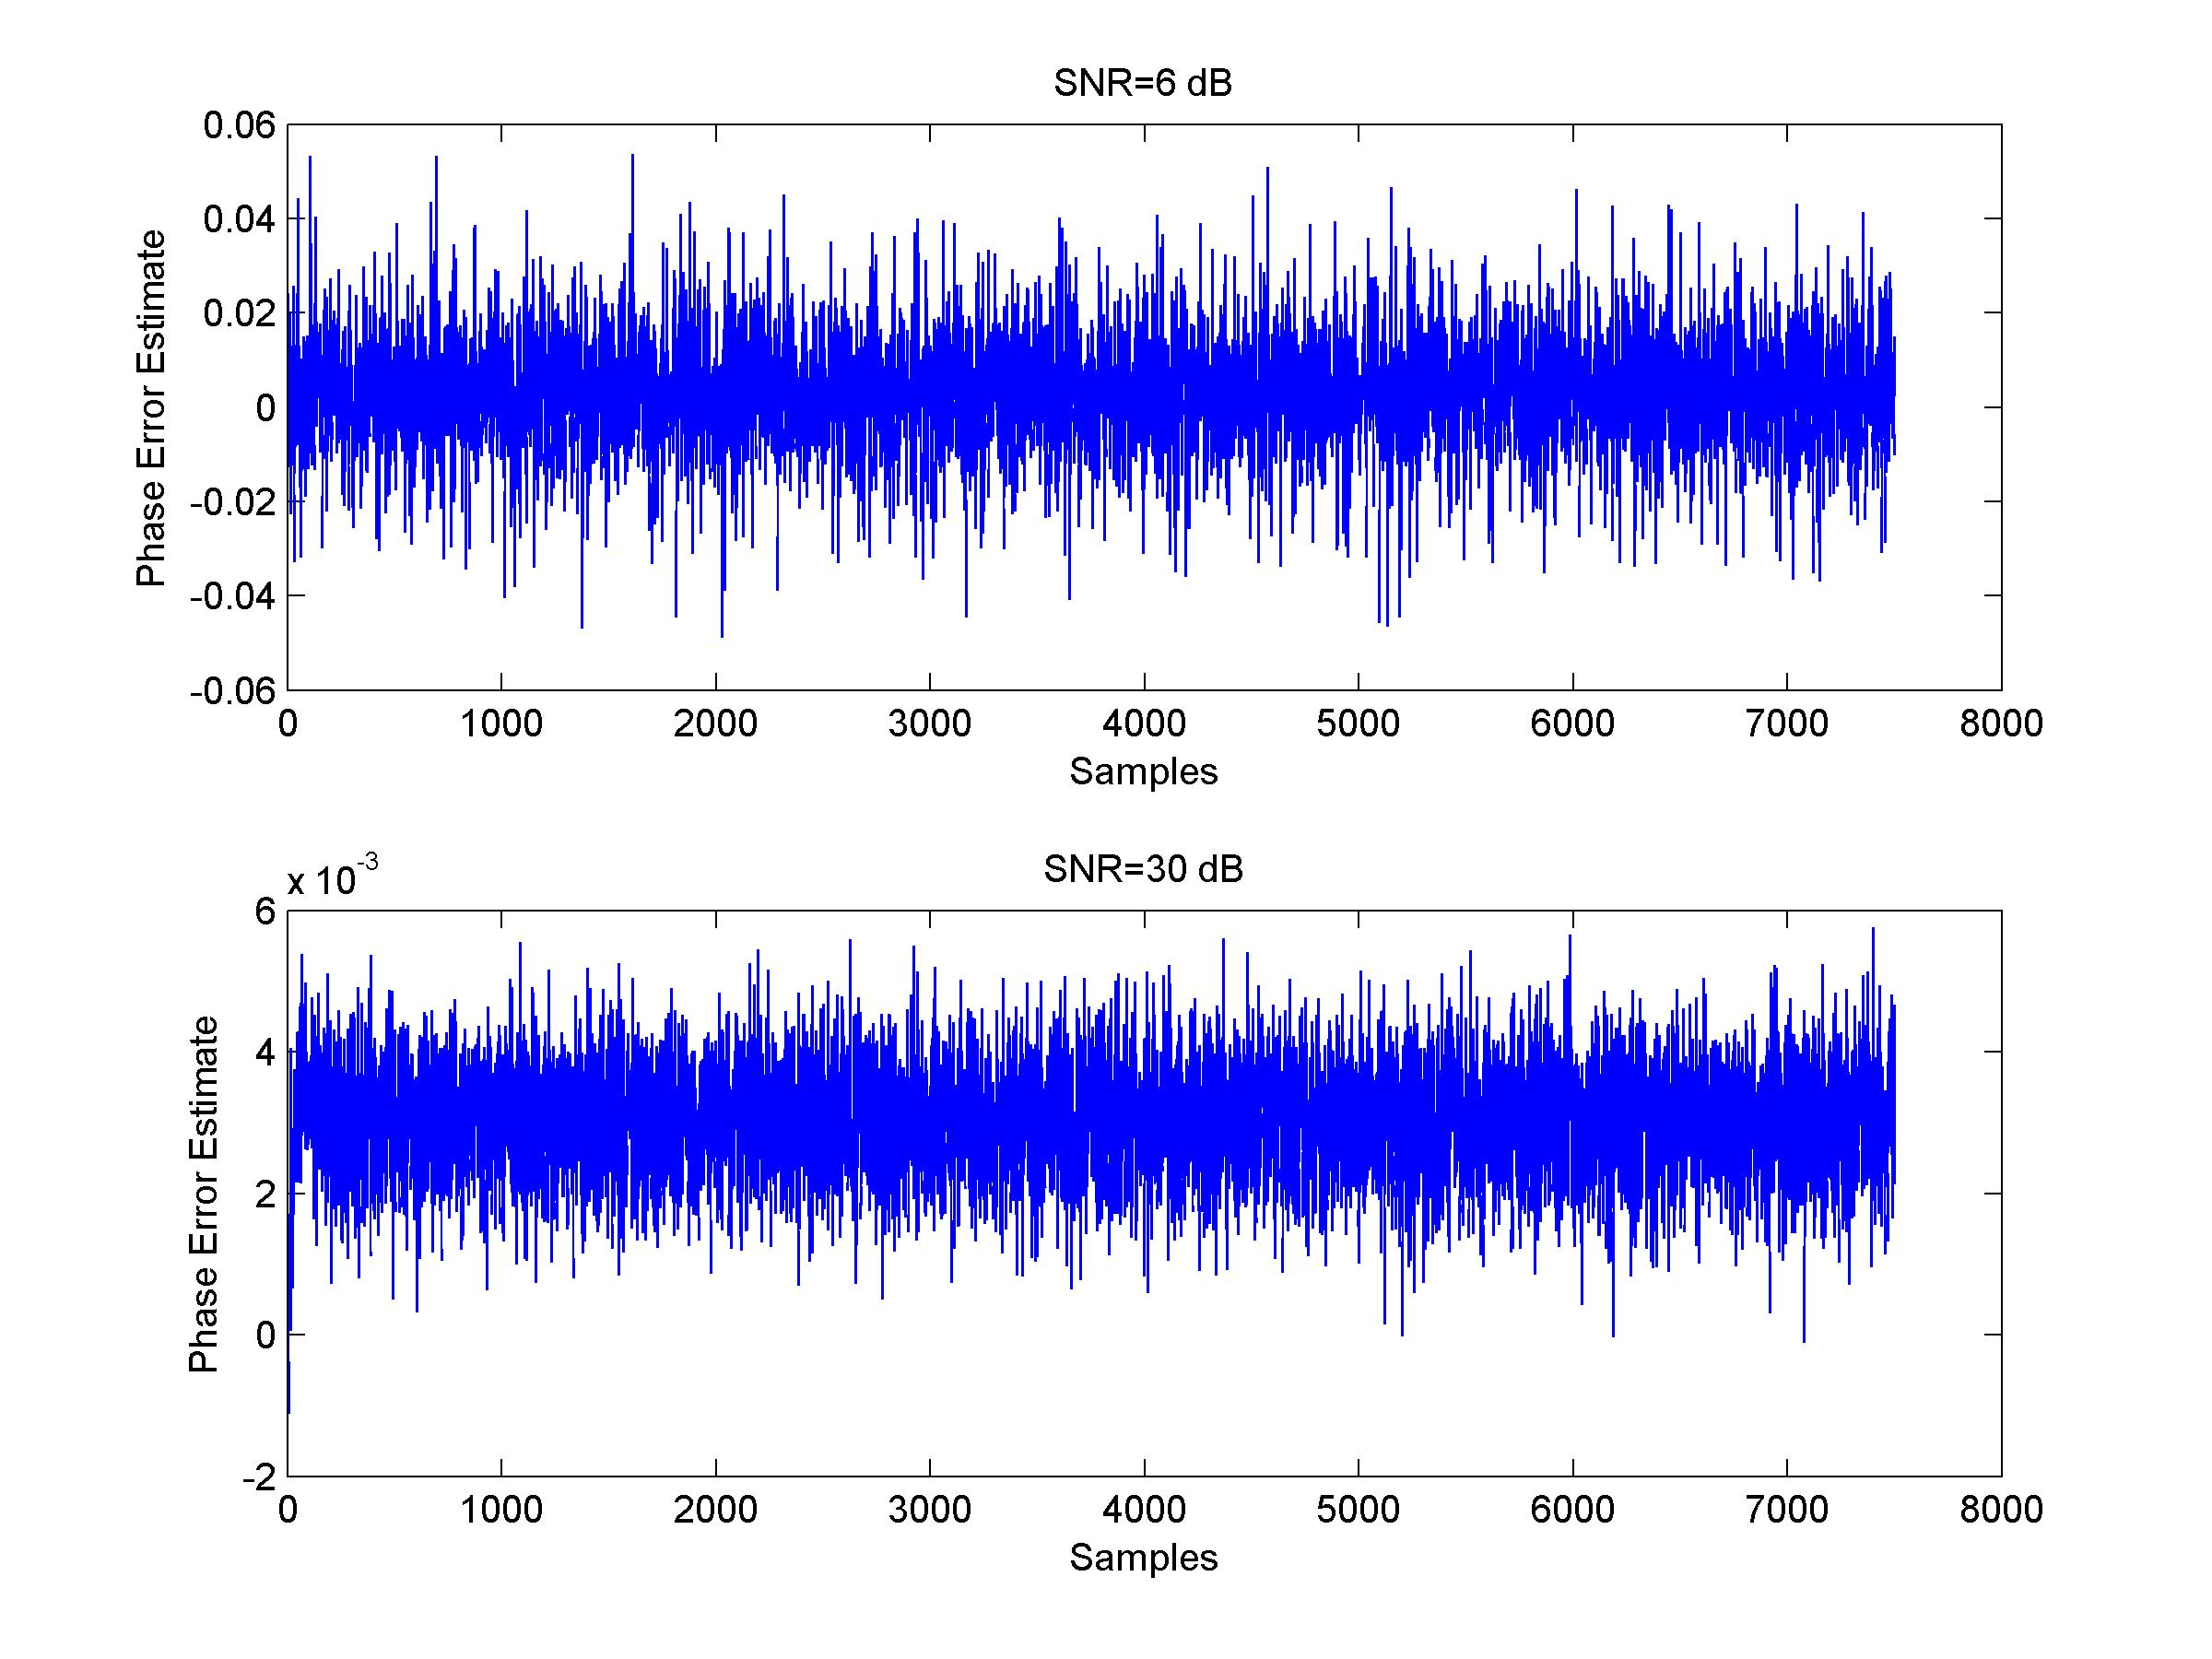
\includegraphics[width=0.5\textwidth]{qpLoopFilterfo_costas2.jpg}
\caption{}
\end{figure}
\subsubsection{Constellation Plots  for Phase Recovery}
\begin{figure}[H]
\centering
\hspace*{-2cm}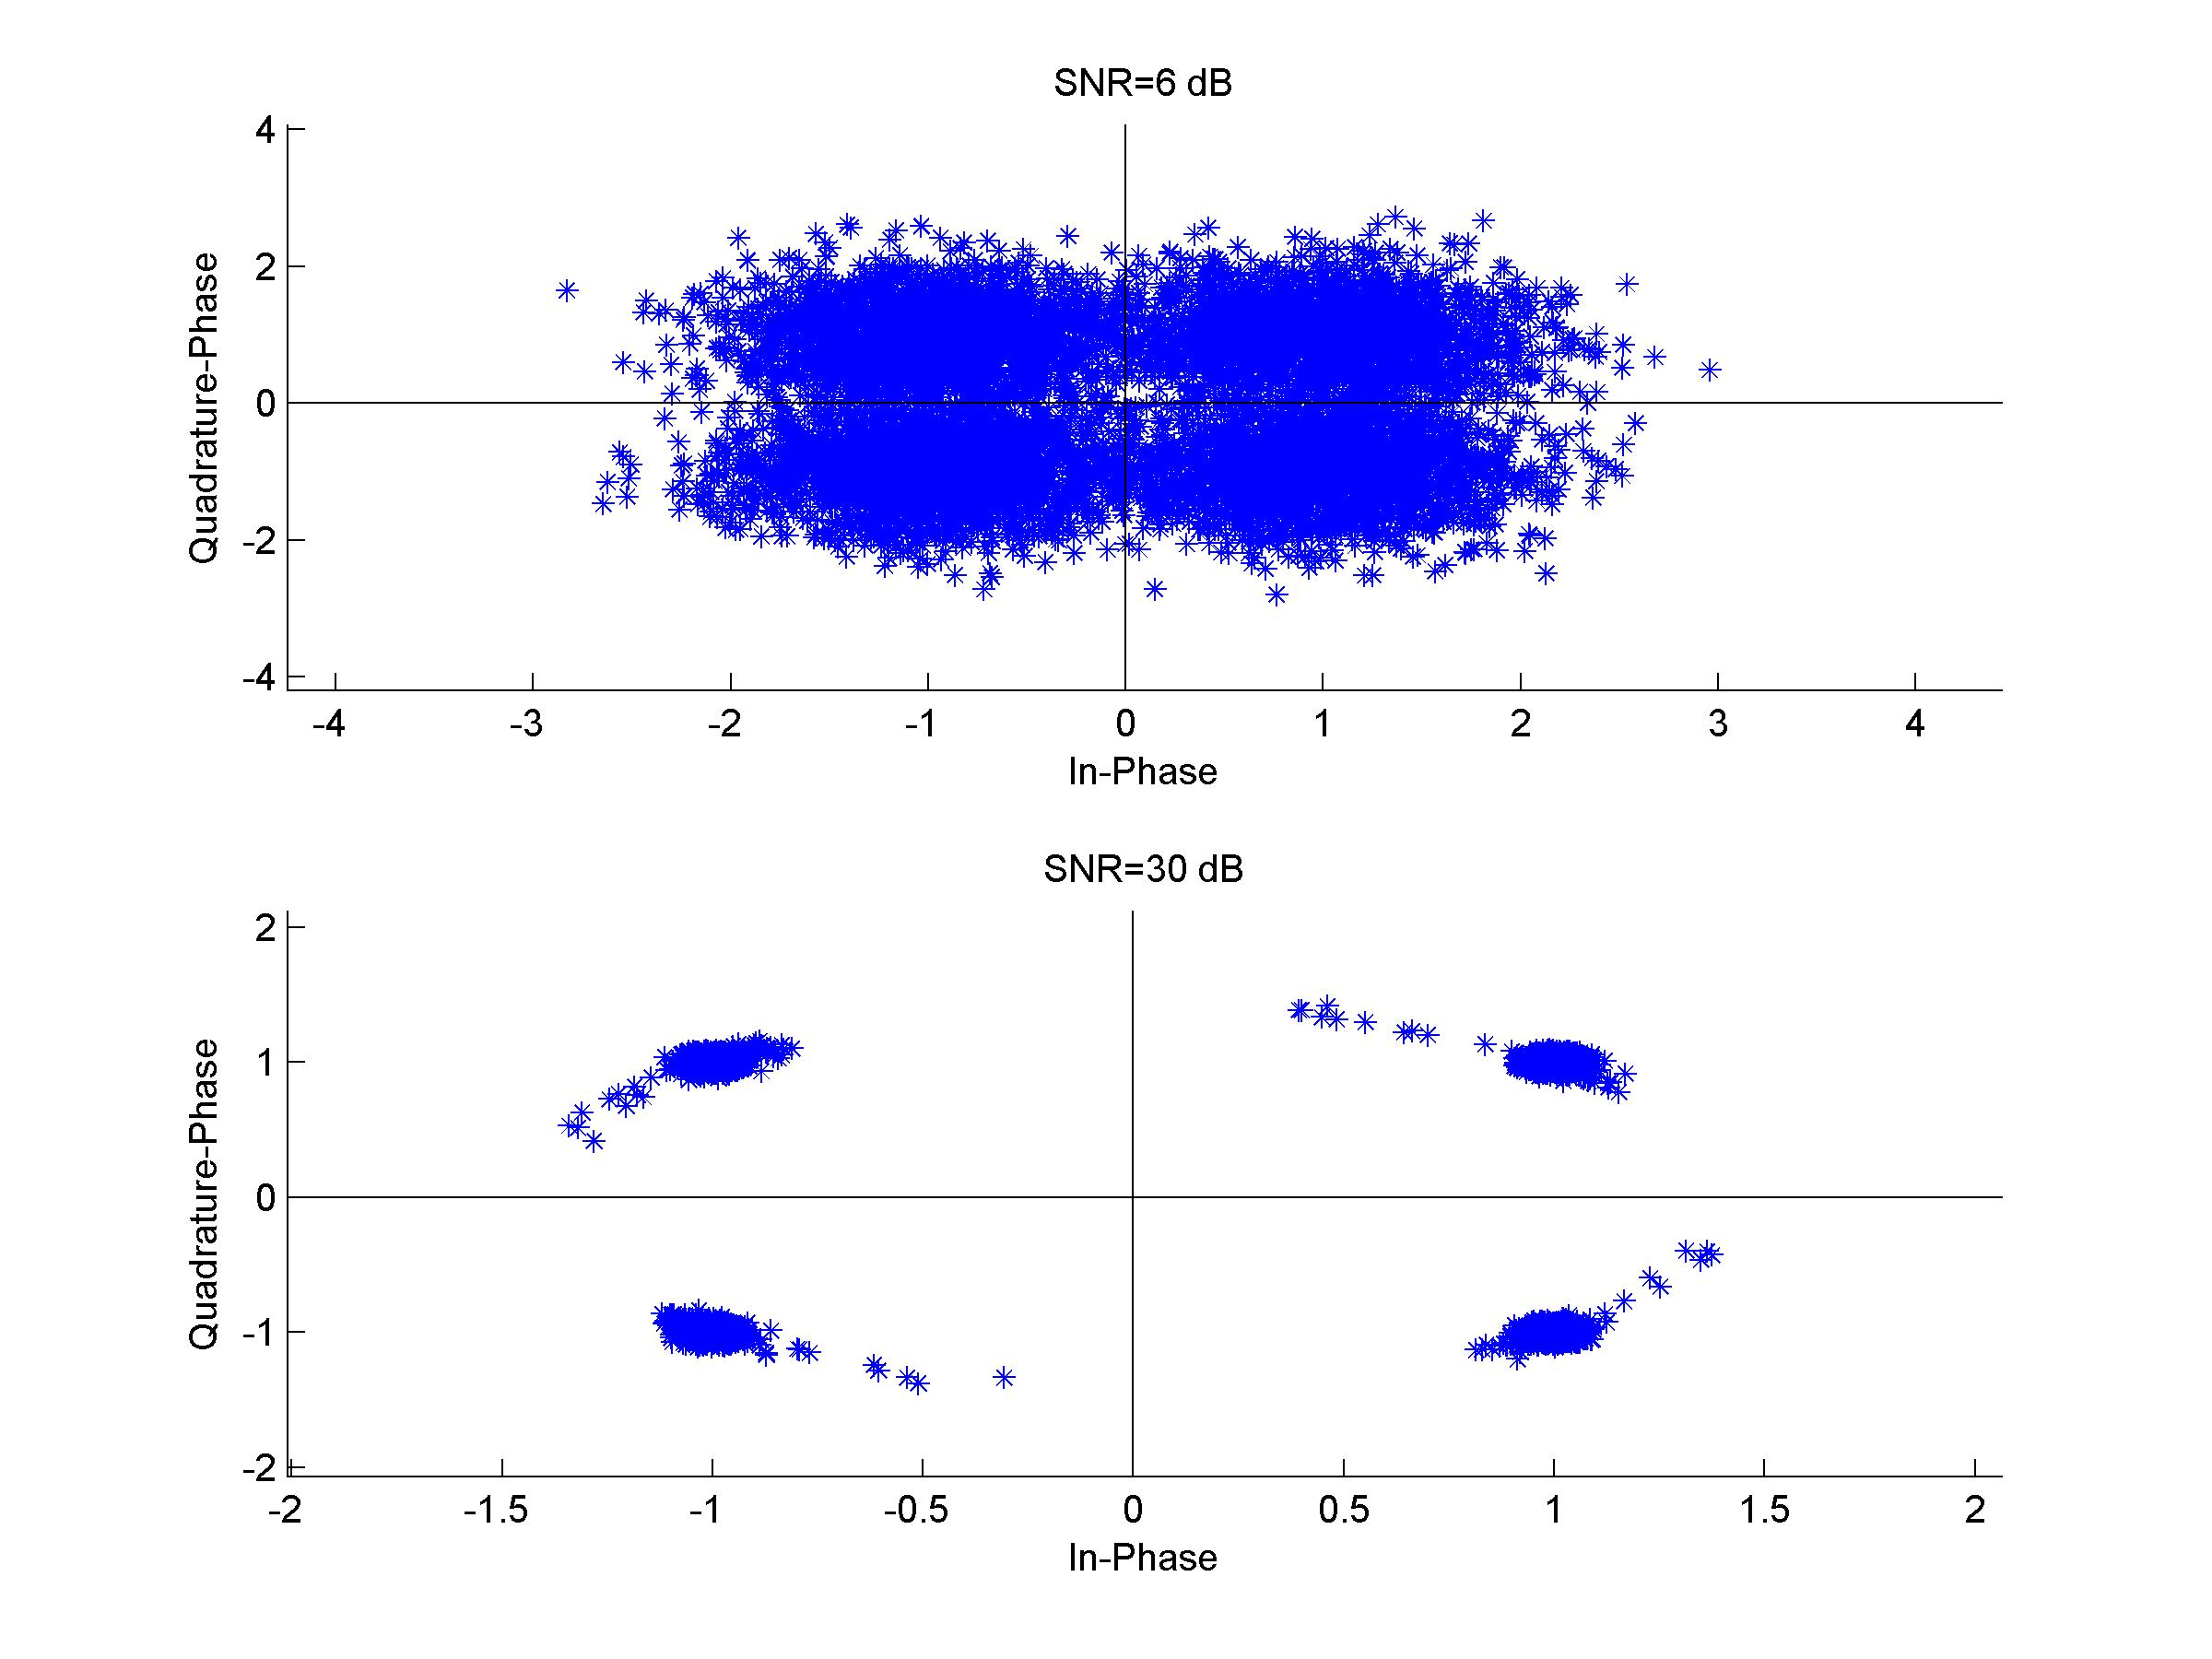
\includegraphics[width=0.5\textwidth]{qpConstpo_costas1.jpg}
\caption{}
\end{figure}

\subsubsection{BER Plots for Carrier Recovery}
\begin{figure}[H]
\centering
\hspace*{-2cm}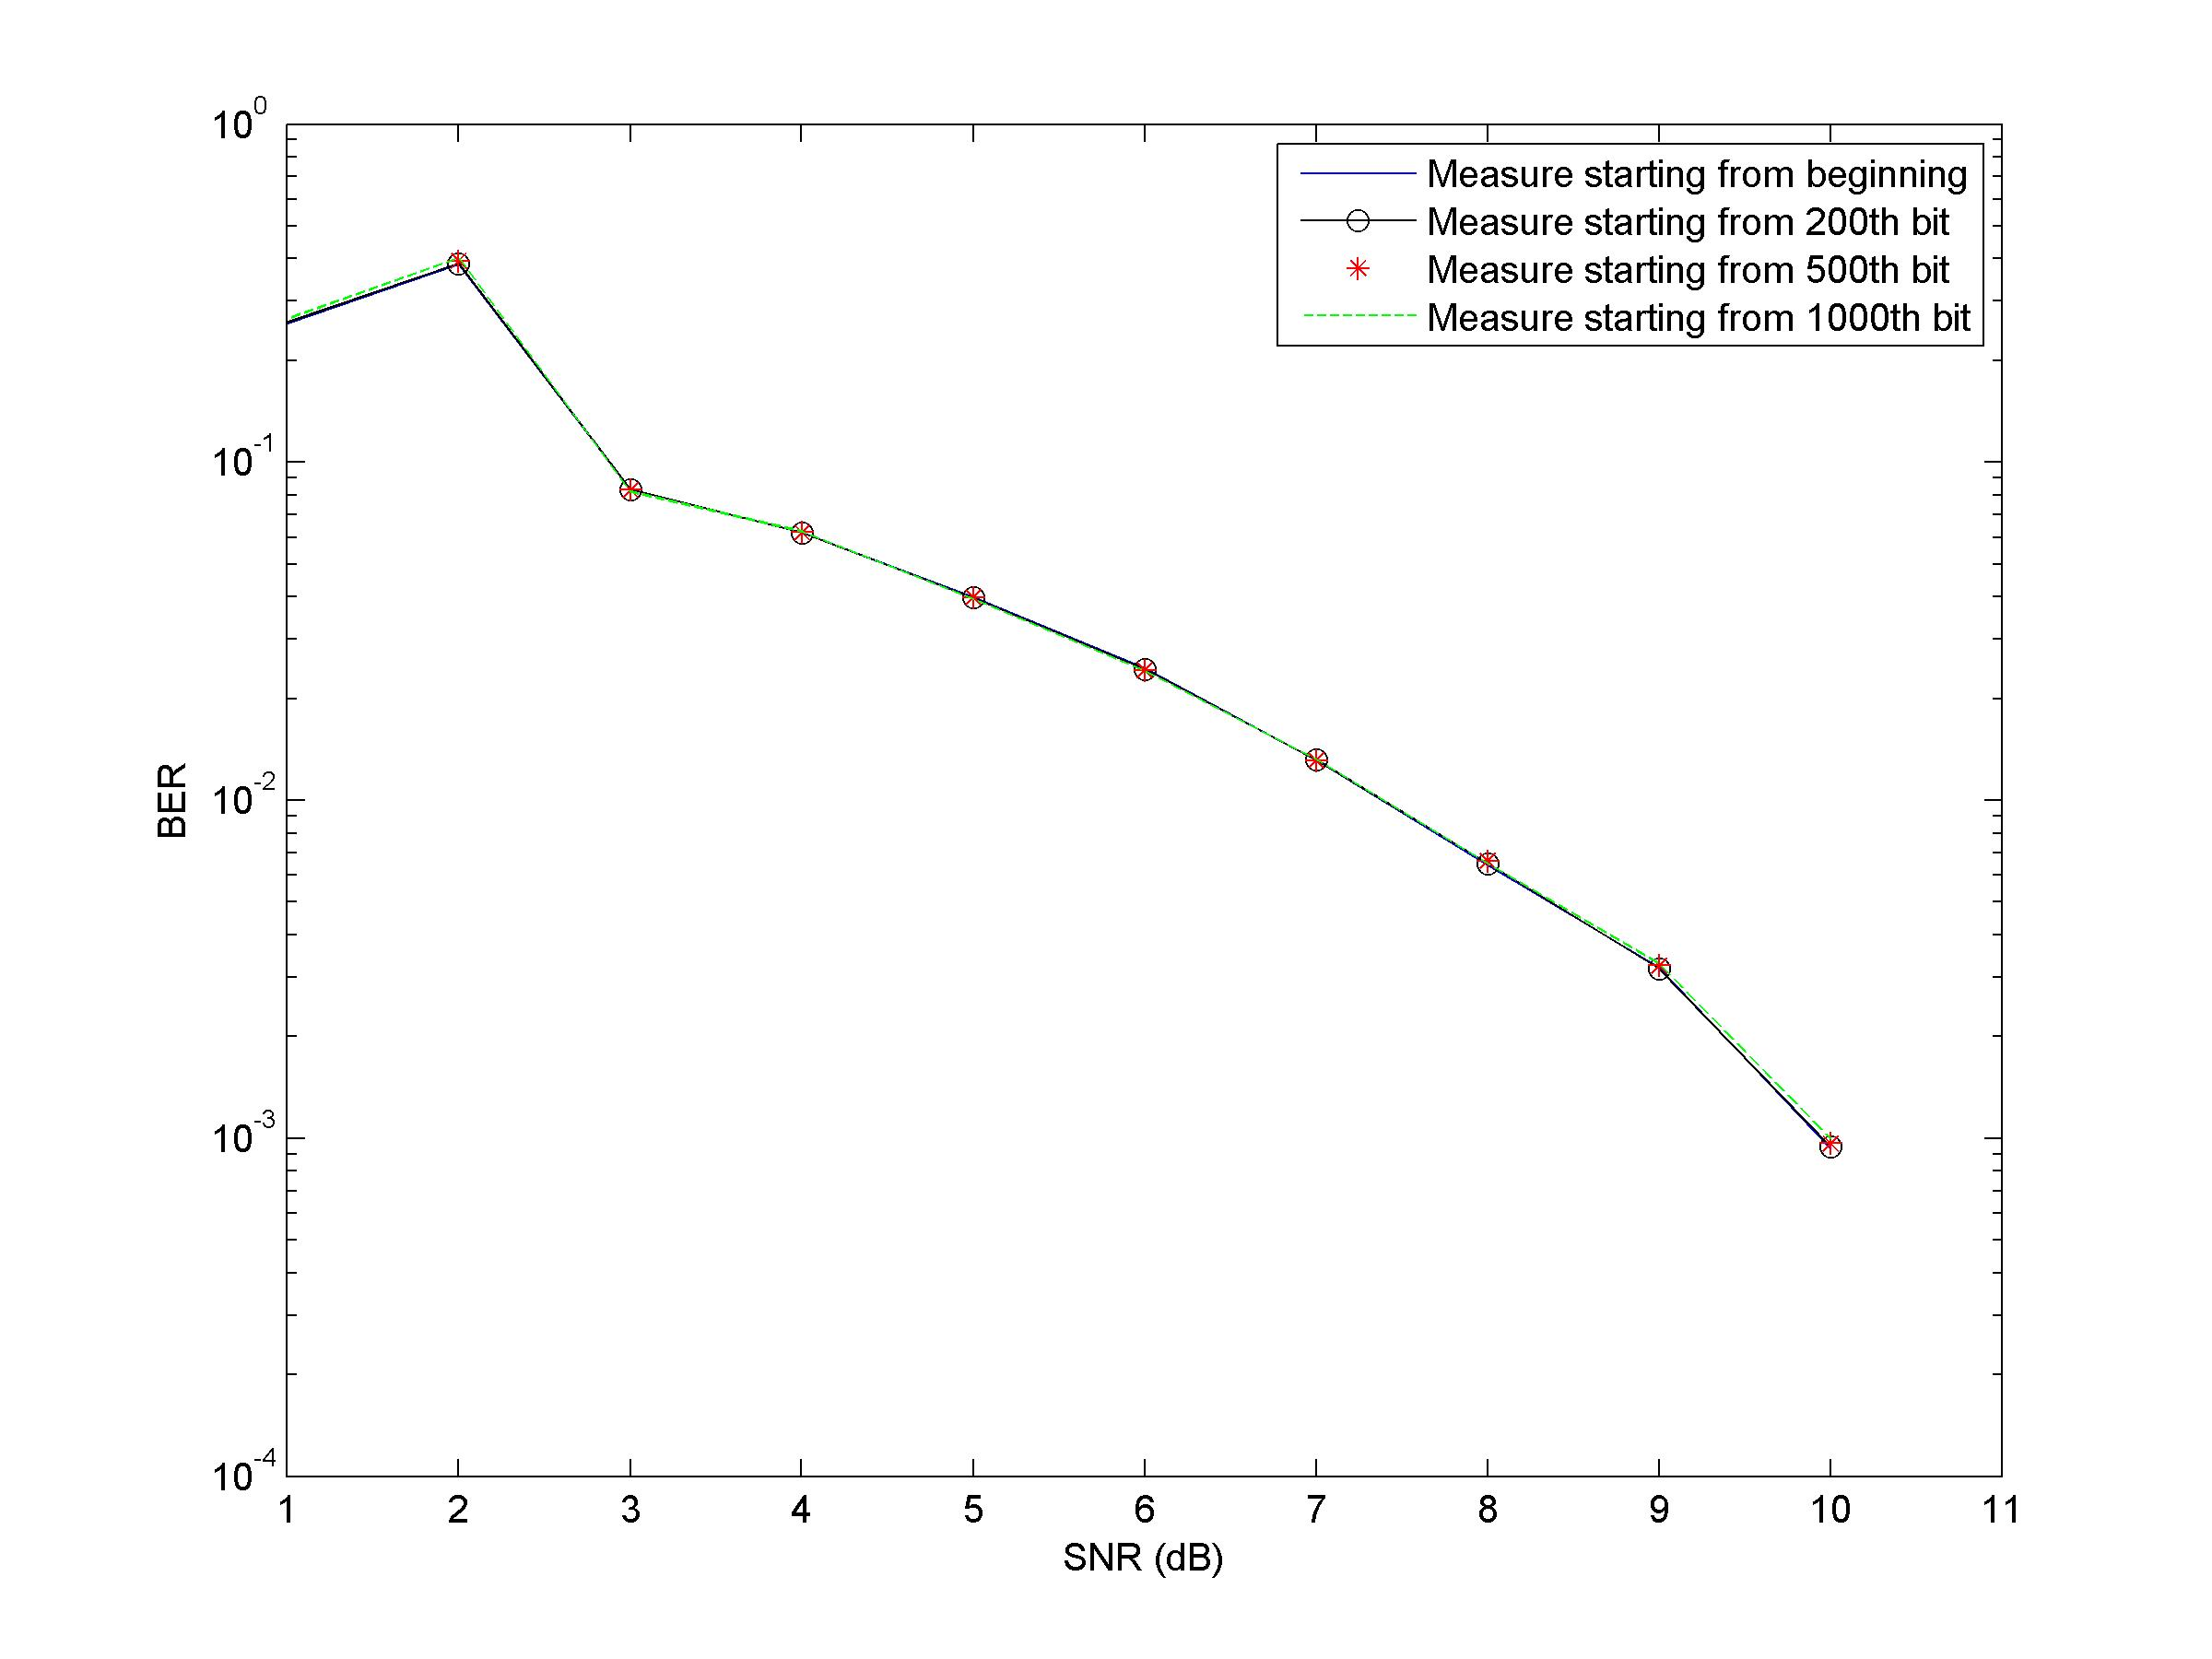
\includegraphics[width=0.5\textwidth]{qpBERfo_costas1.jpg}
\caption{}
\end{figure}

\begin{figure}[H]
\centering
\hspace*{-2cm}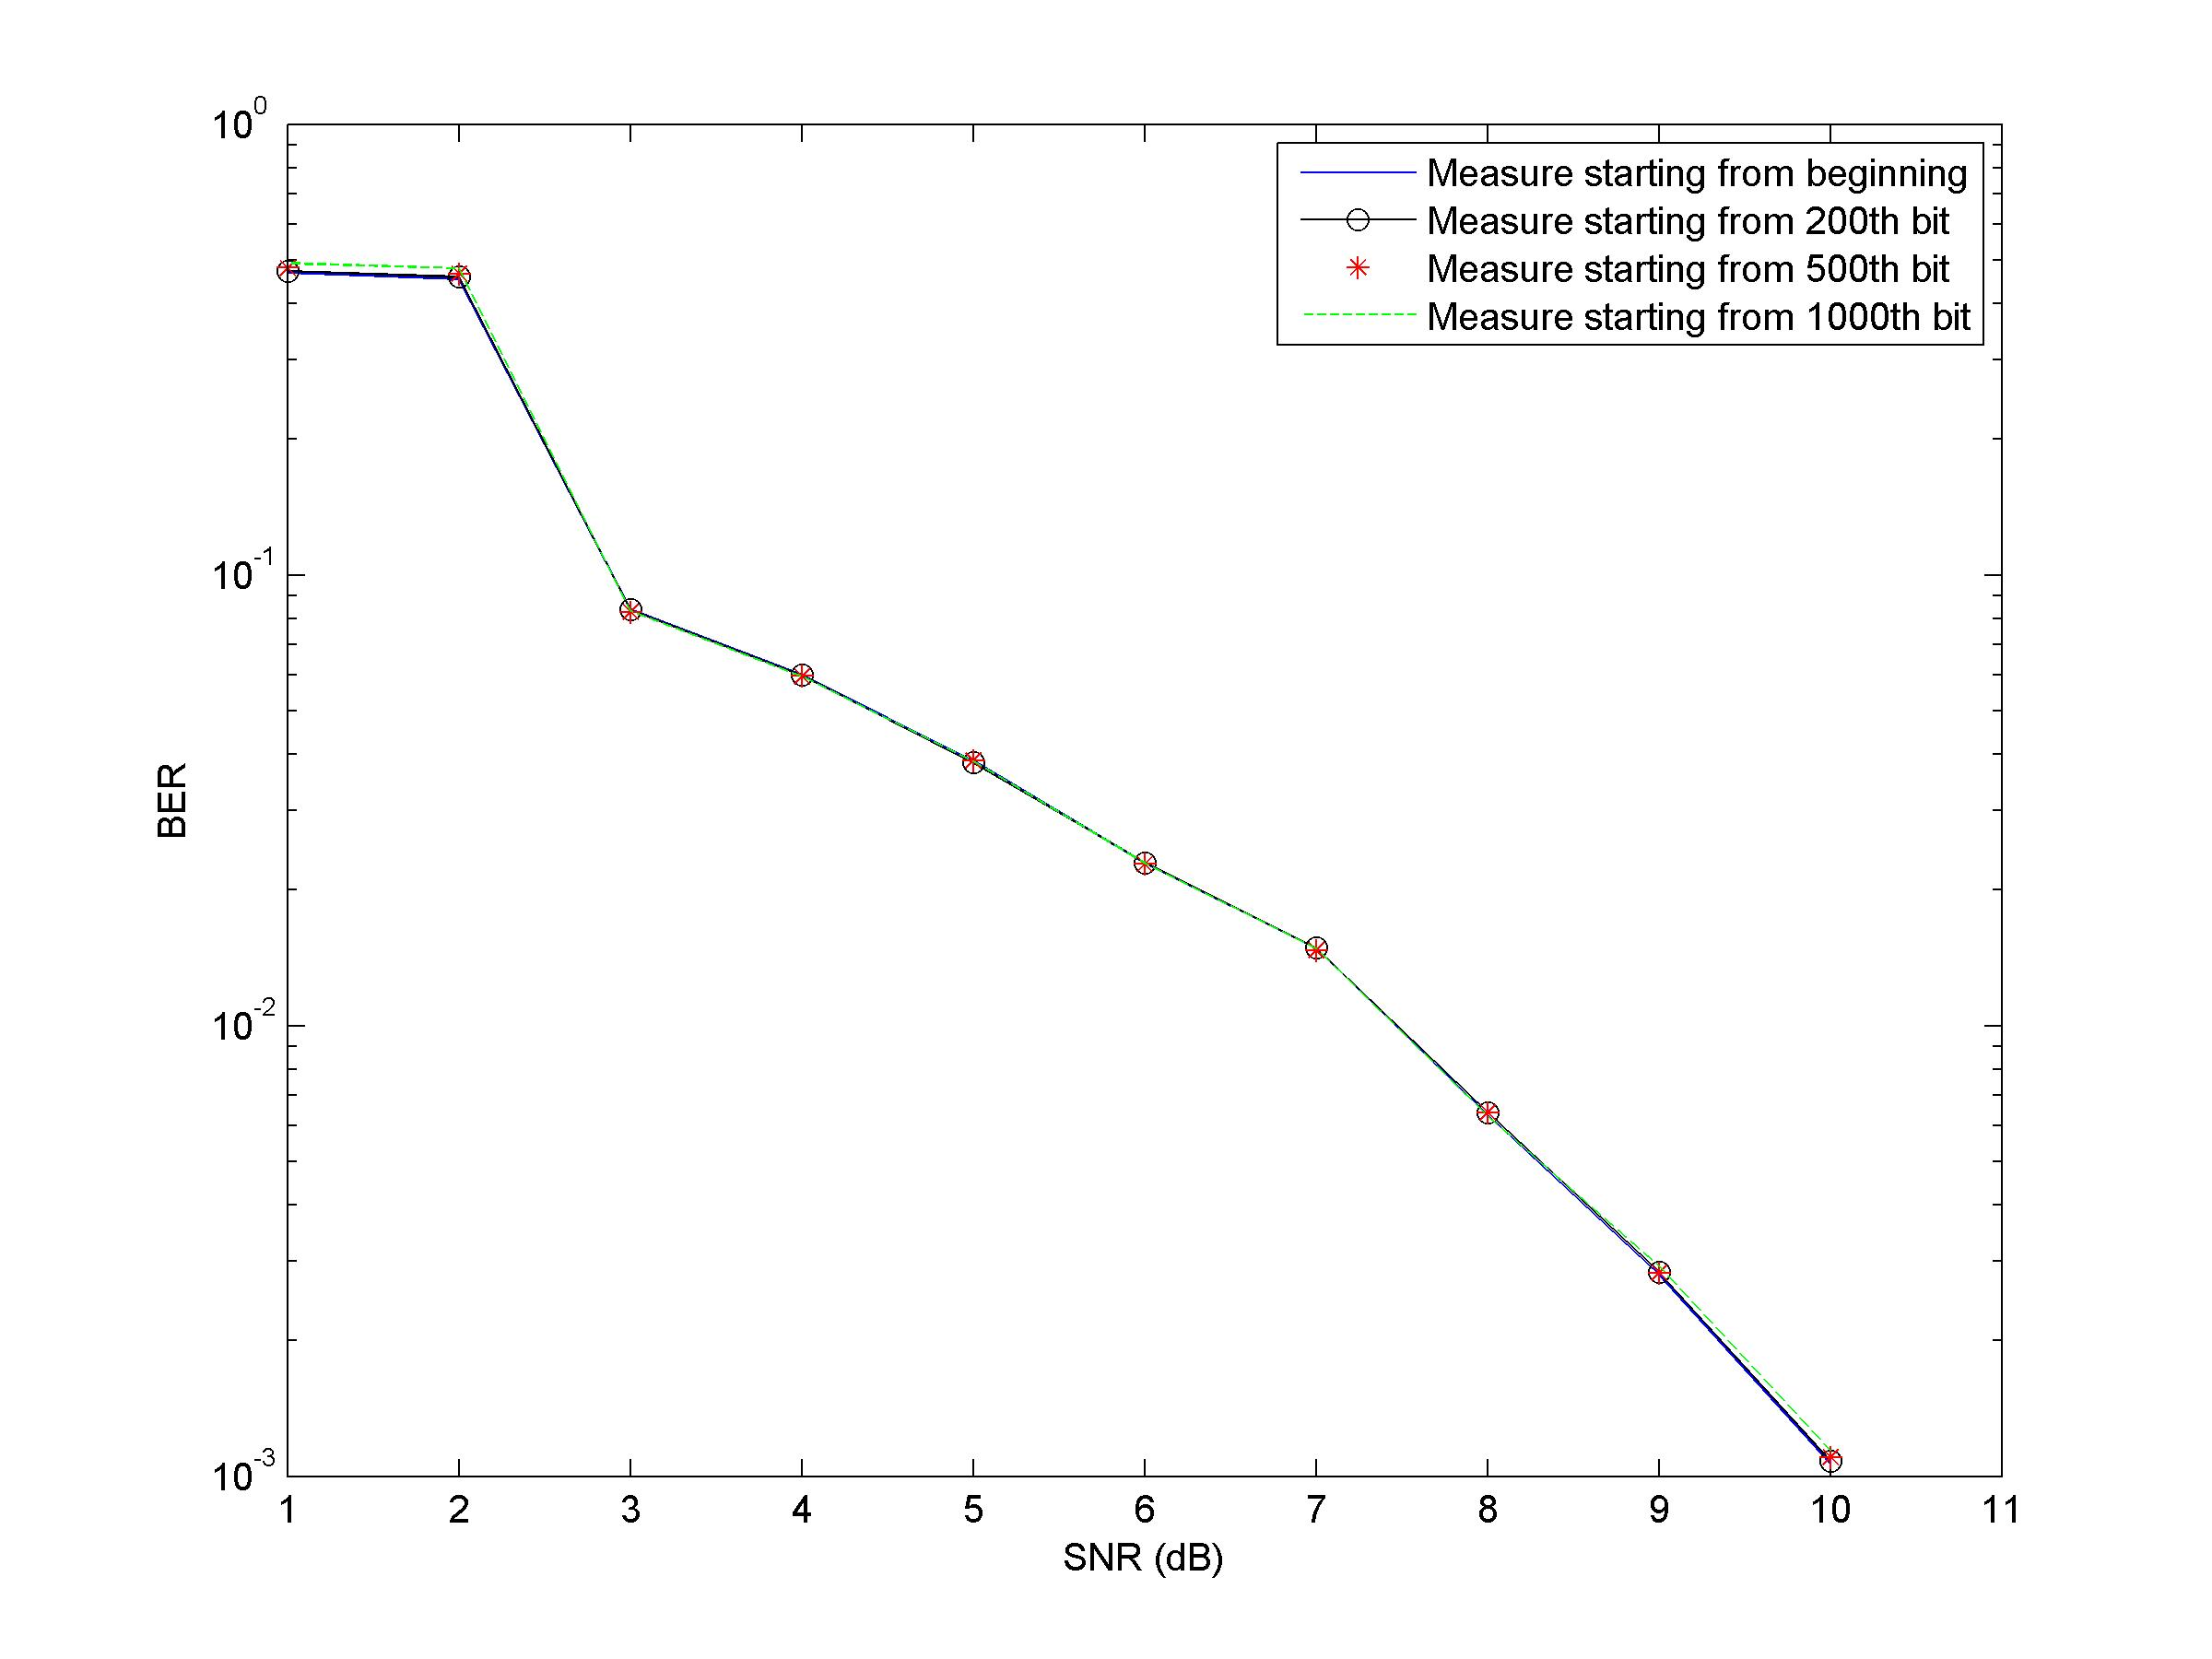
\includegraphics[width=0.5\textwidth]{qpBERfo_costas2.jpg}
\caption{}
\end{figure}

\subsubsection{BER Plots for Phase Recovery}
\begin{figure}[H]
\centering
\hspace*{-2cm}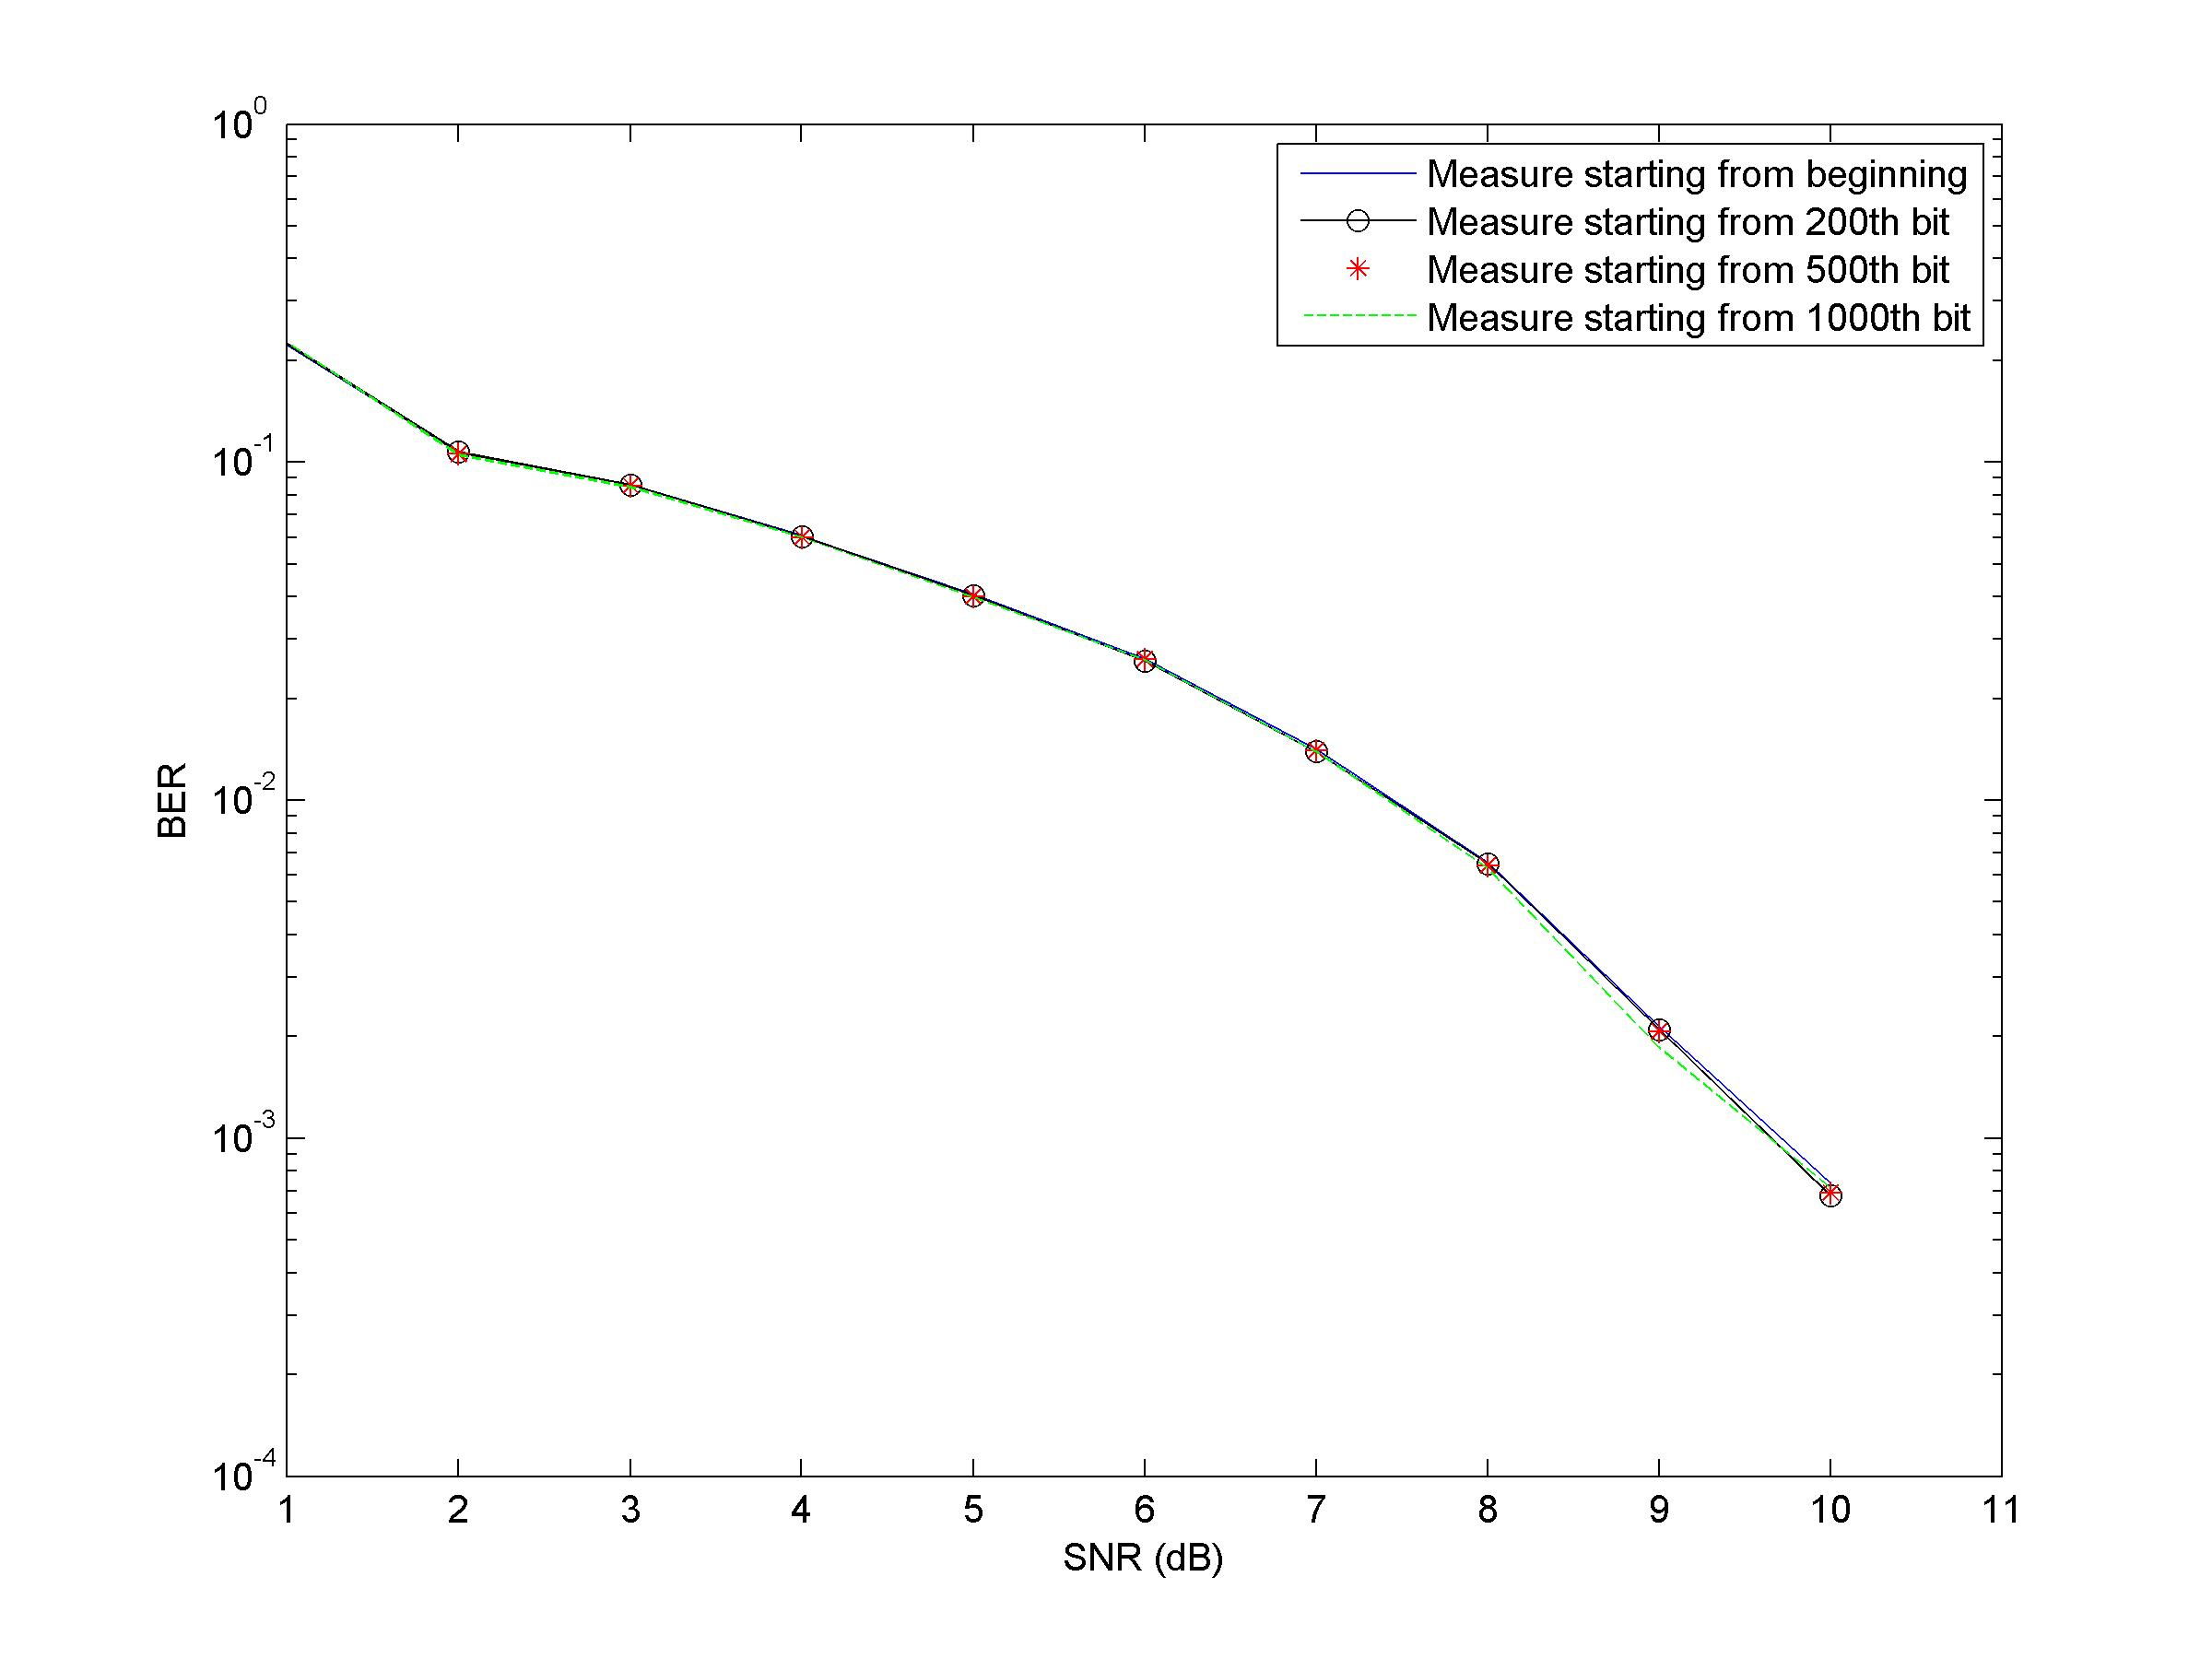
\includegraphics[width=0.5\textwidth]{qpBERpo_costas1.jpg}
\caption{}
\end{figure}

\subsection{QPSK with Decision Directed Recovery}

\subsubsection{S-Curve of Phase Detector}
\begin{figure}[H]
\centering
\hspace*{-2cm}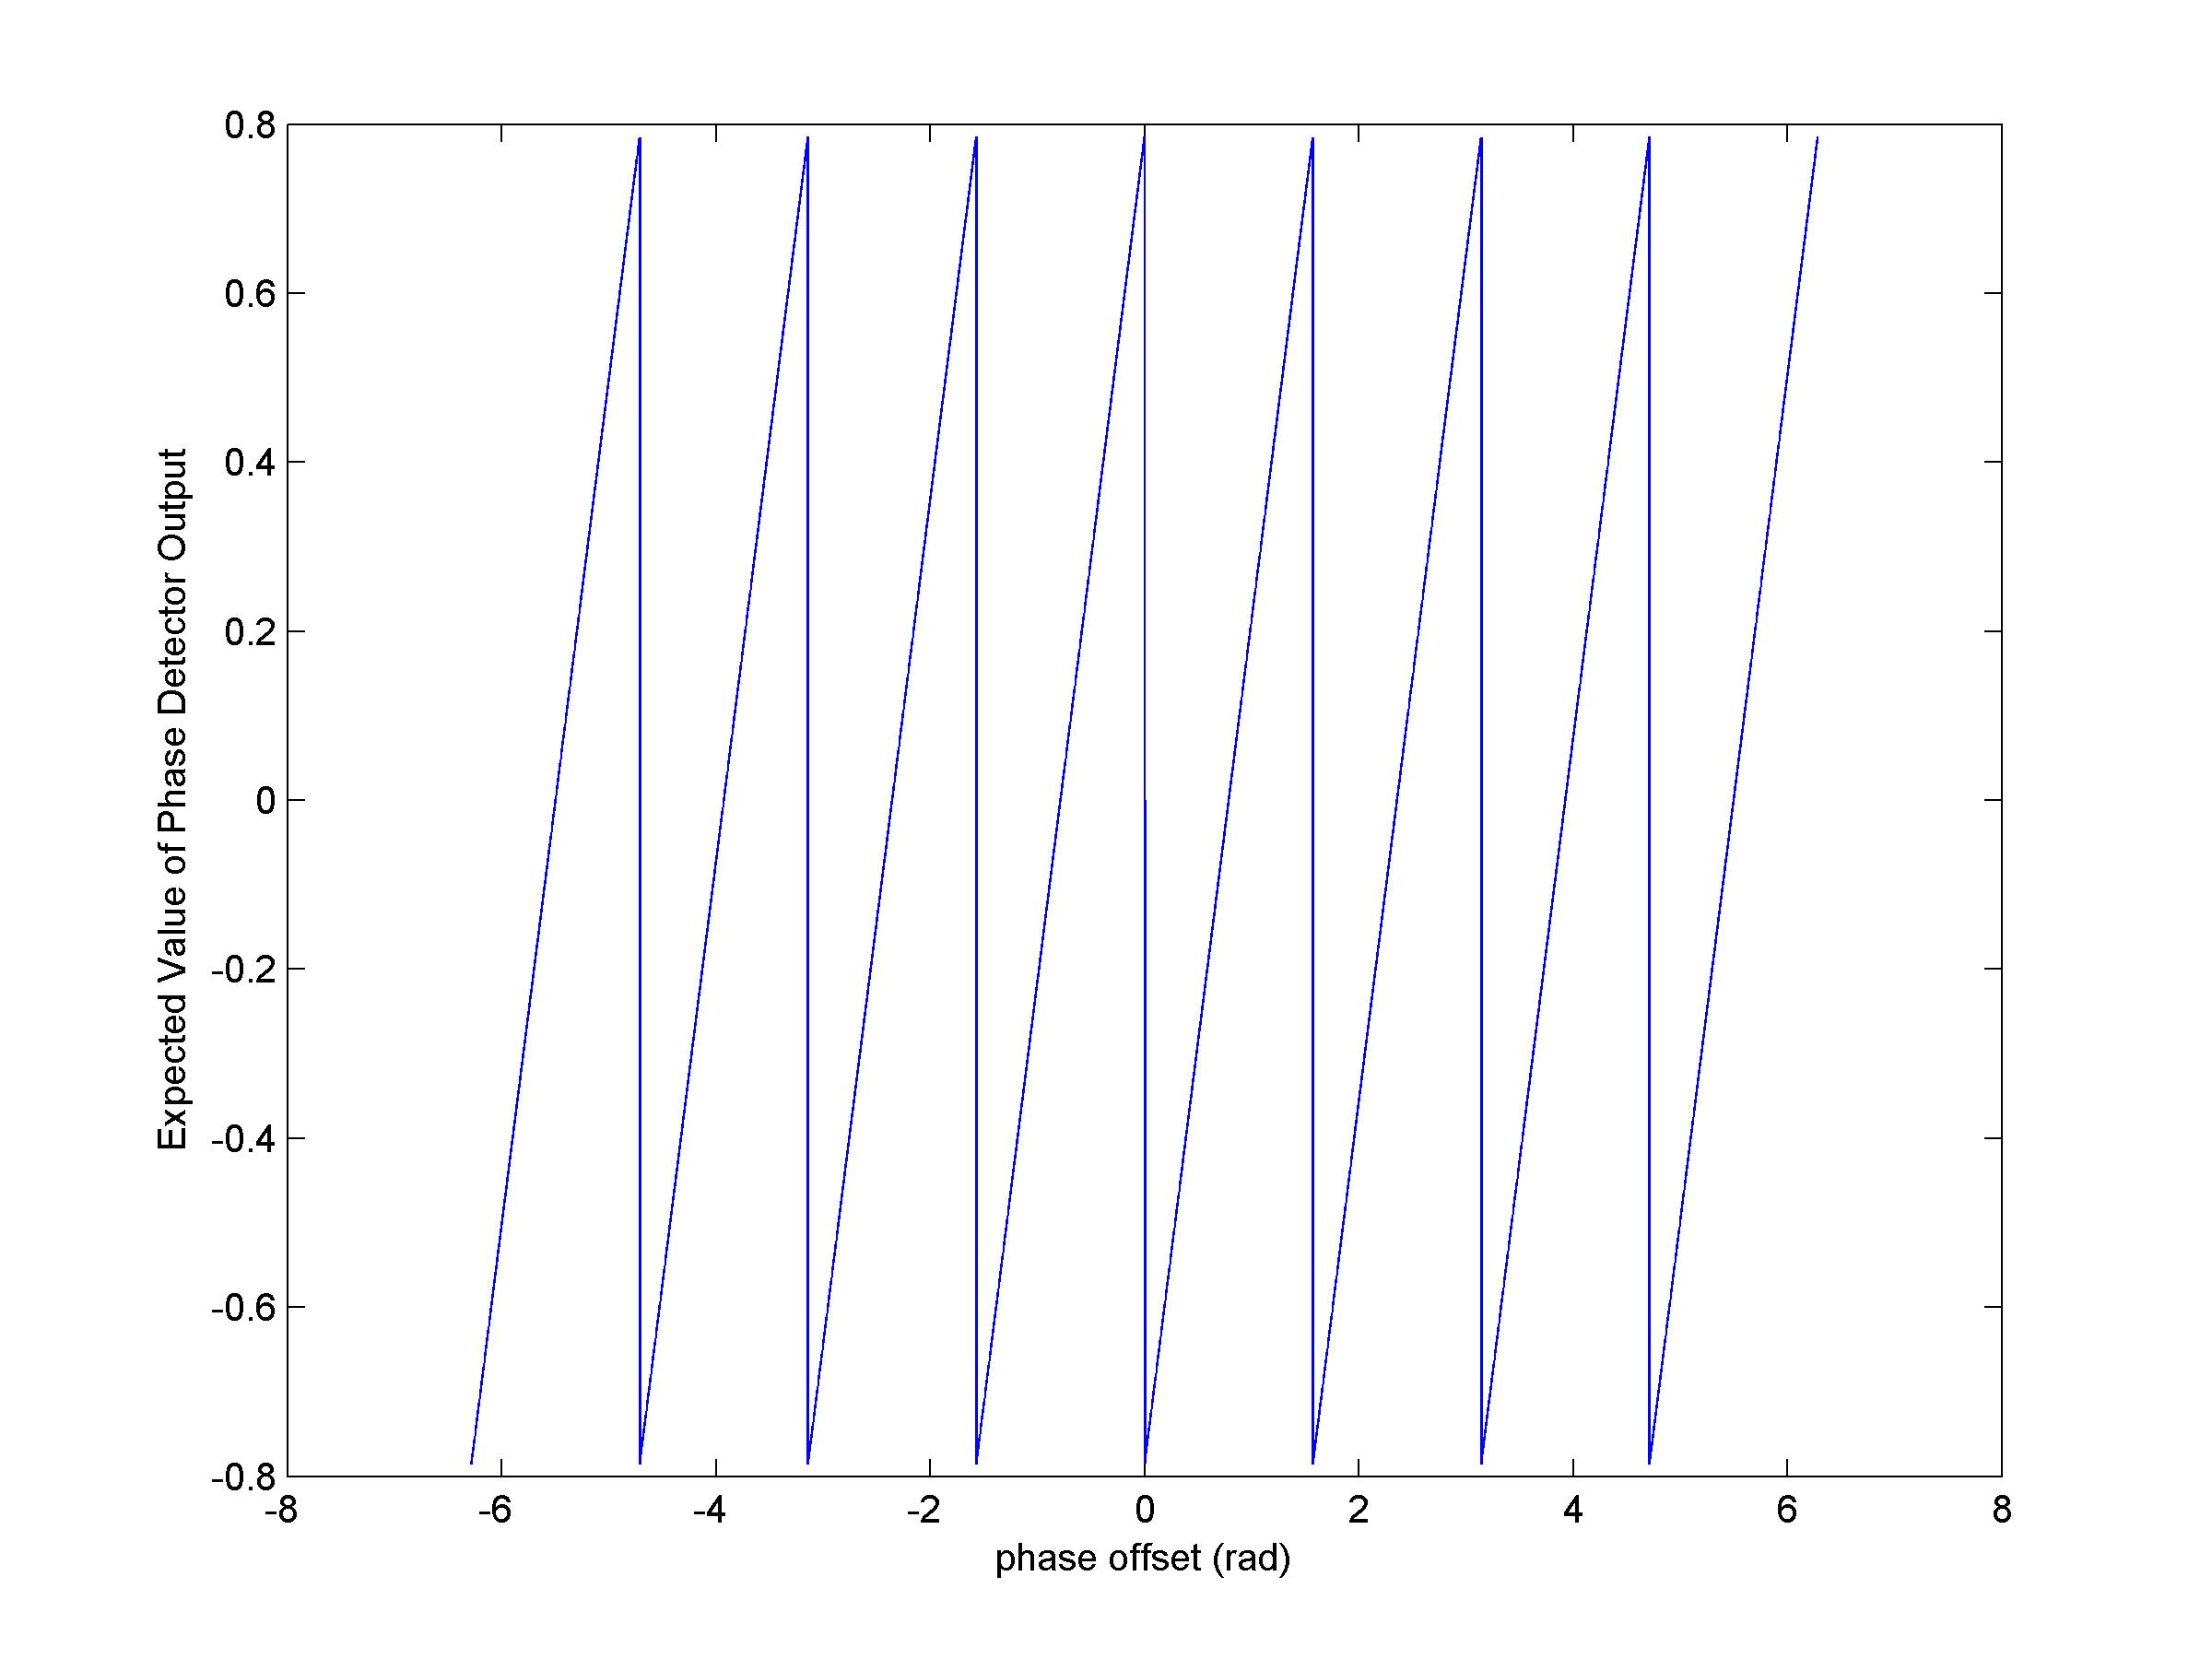
\includegraphics[width=0.5\textwidth]{qpScurvepo_ddr.jpg}
\caption{}
\end{figure}
\subsubsection{S-Curve of Carrier Detector}
\begin{figure}[H]
\centering
\hspace*{-2cm}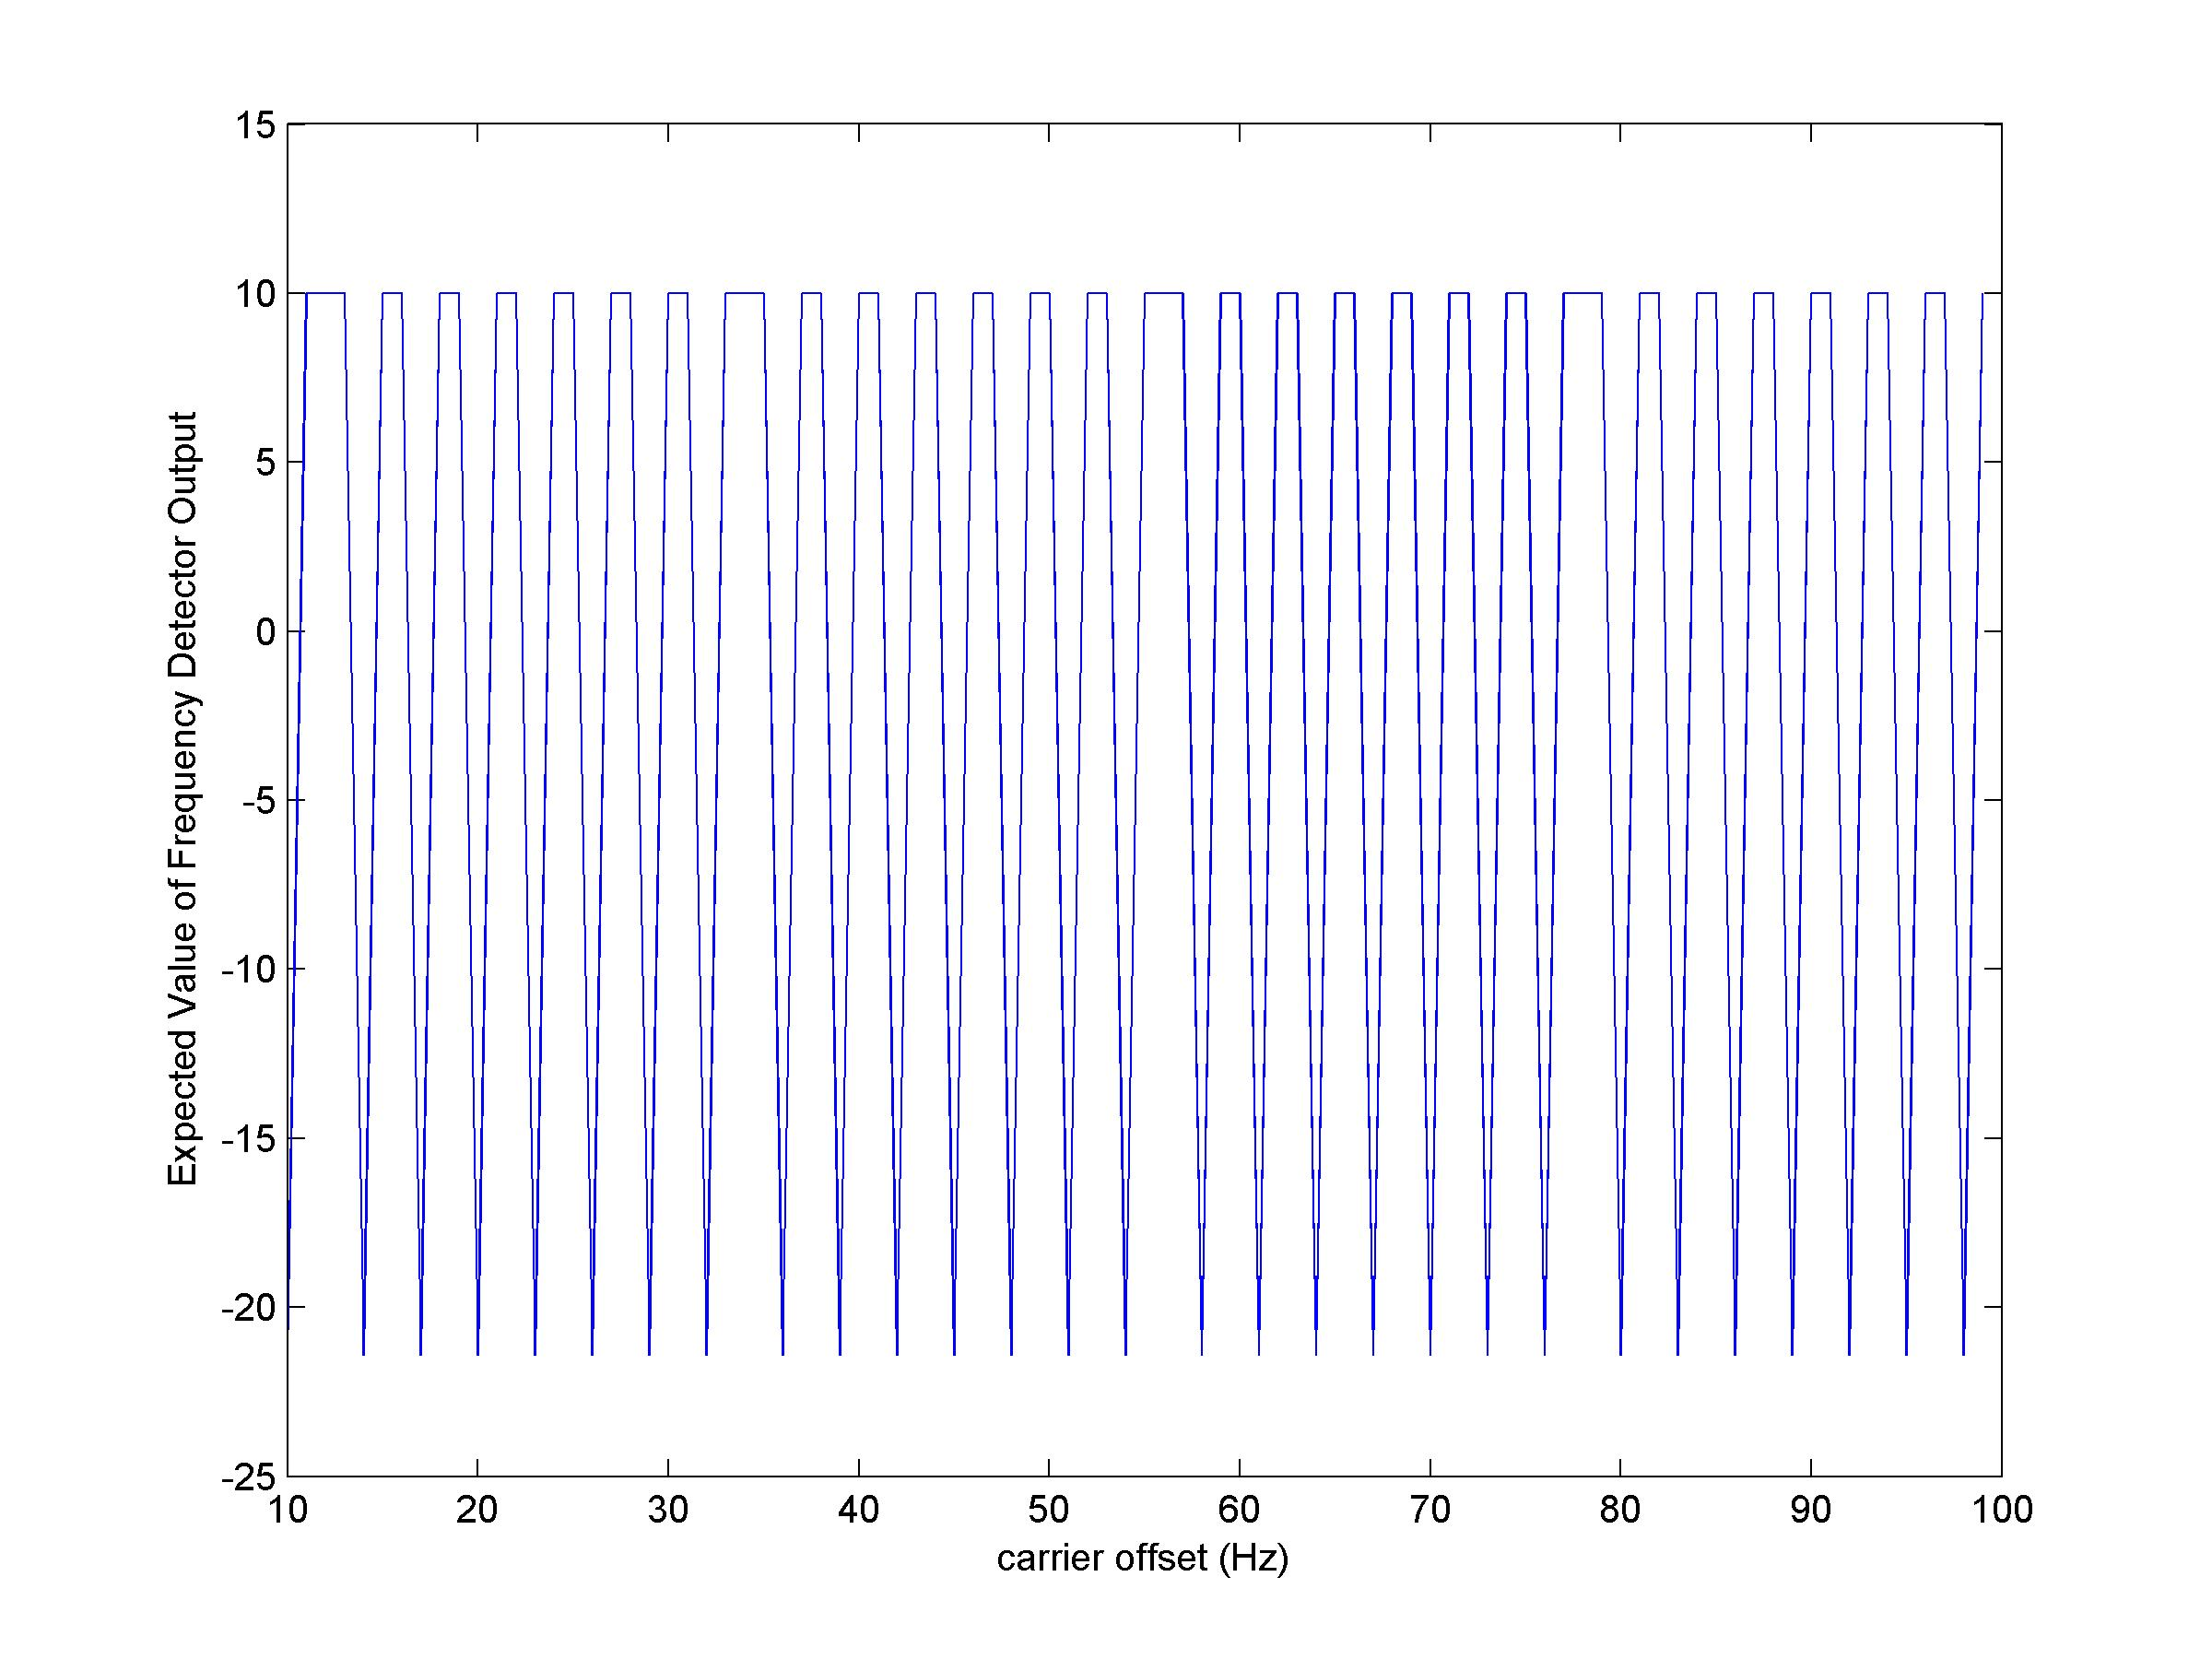
\includegraphics[width=0.5\textwidth]{qpScurvefo.jpg}
\caption{}
\end{figure}
\subsubsection{Transience of Phase Recovery}
\begin{figure}[H]
\centering
\hspace*{-2cm}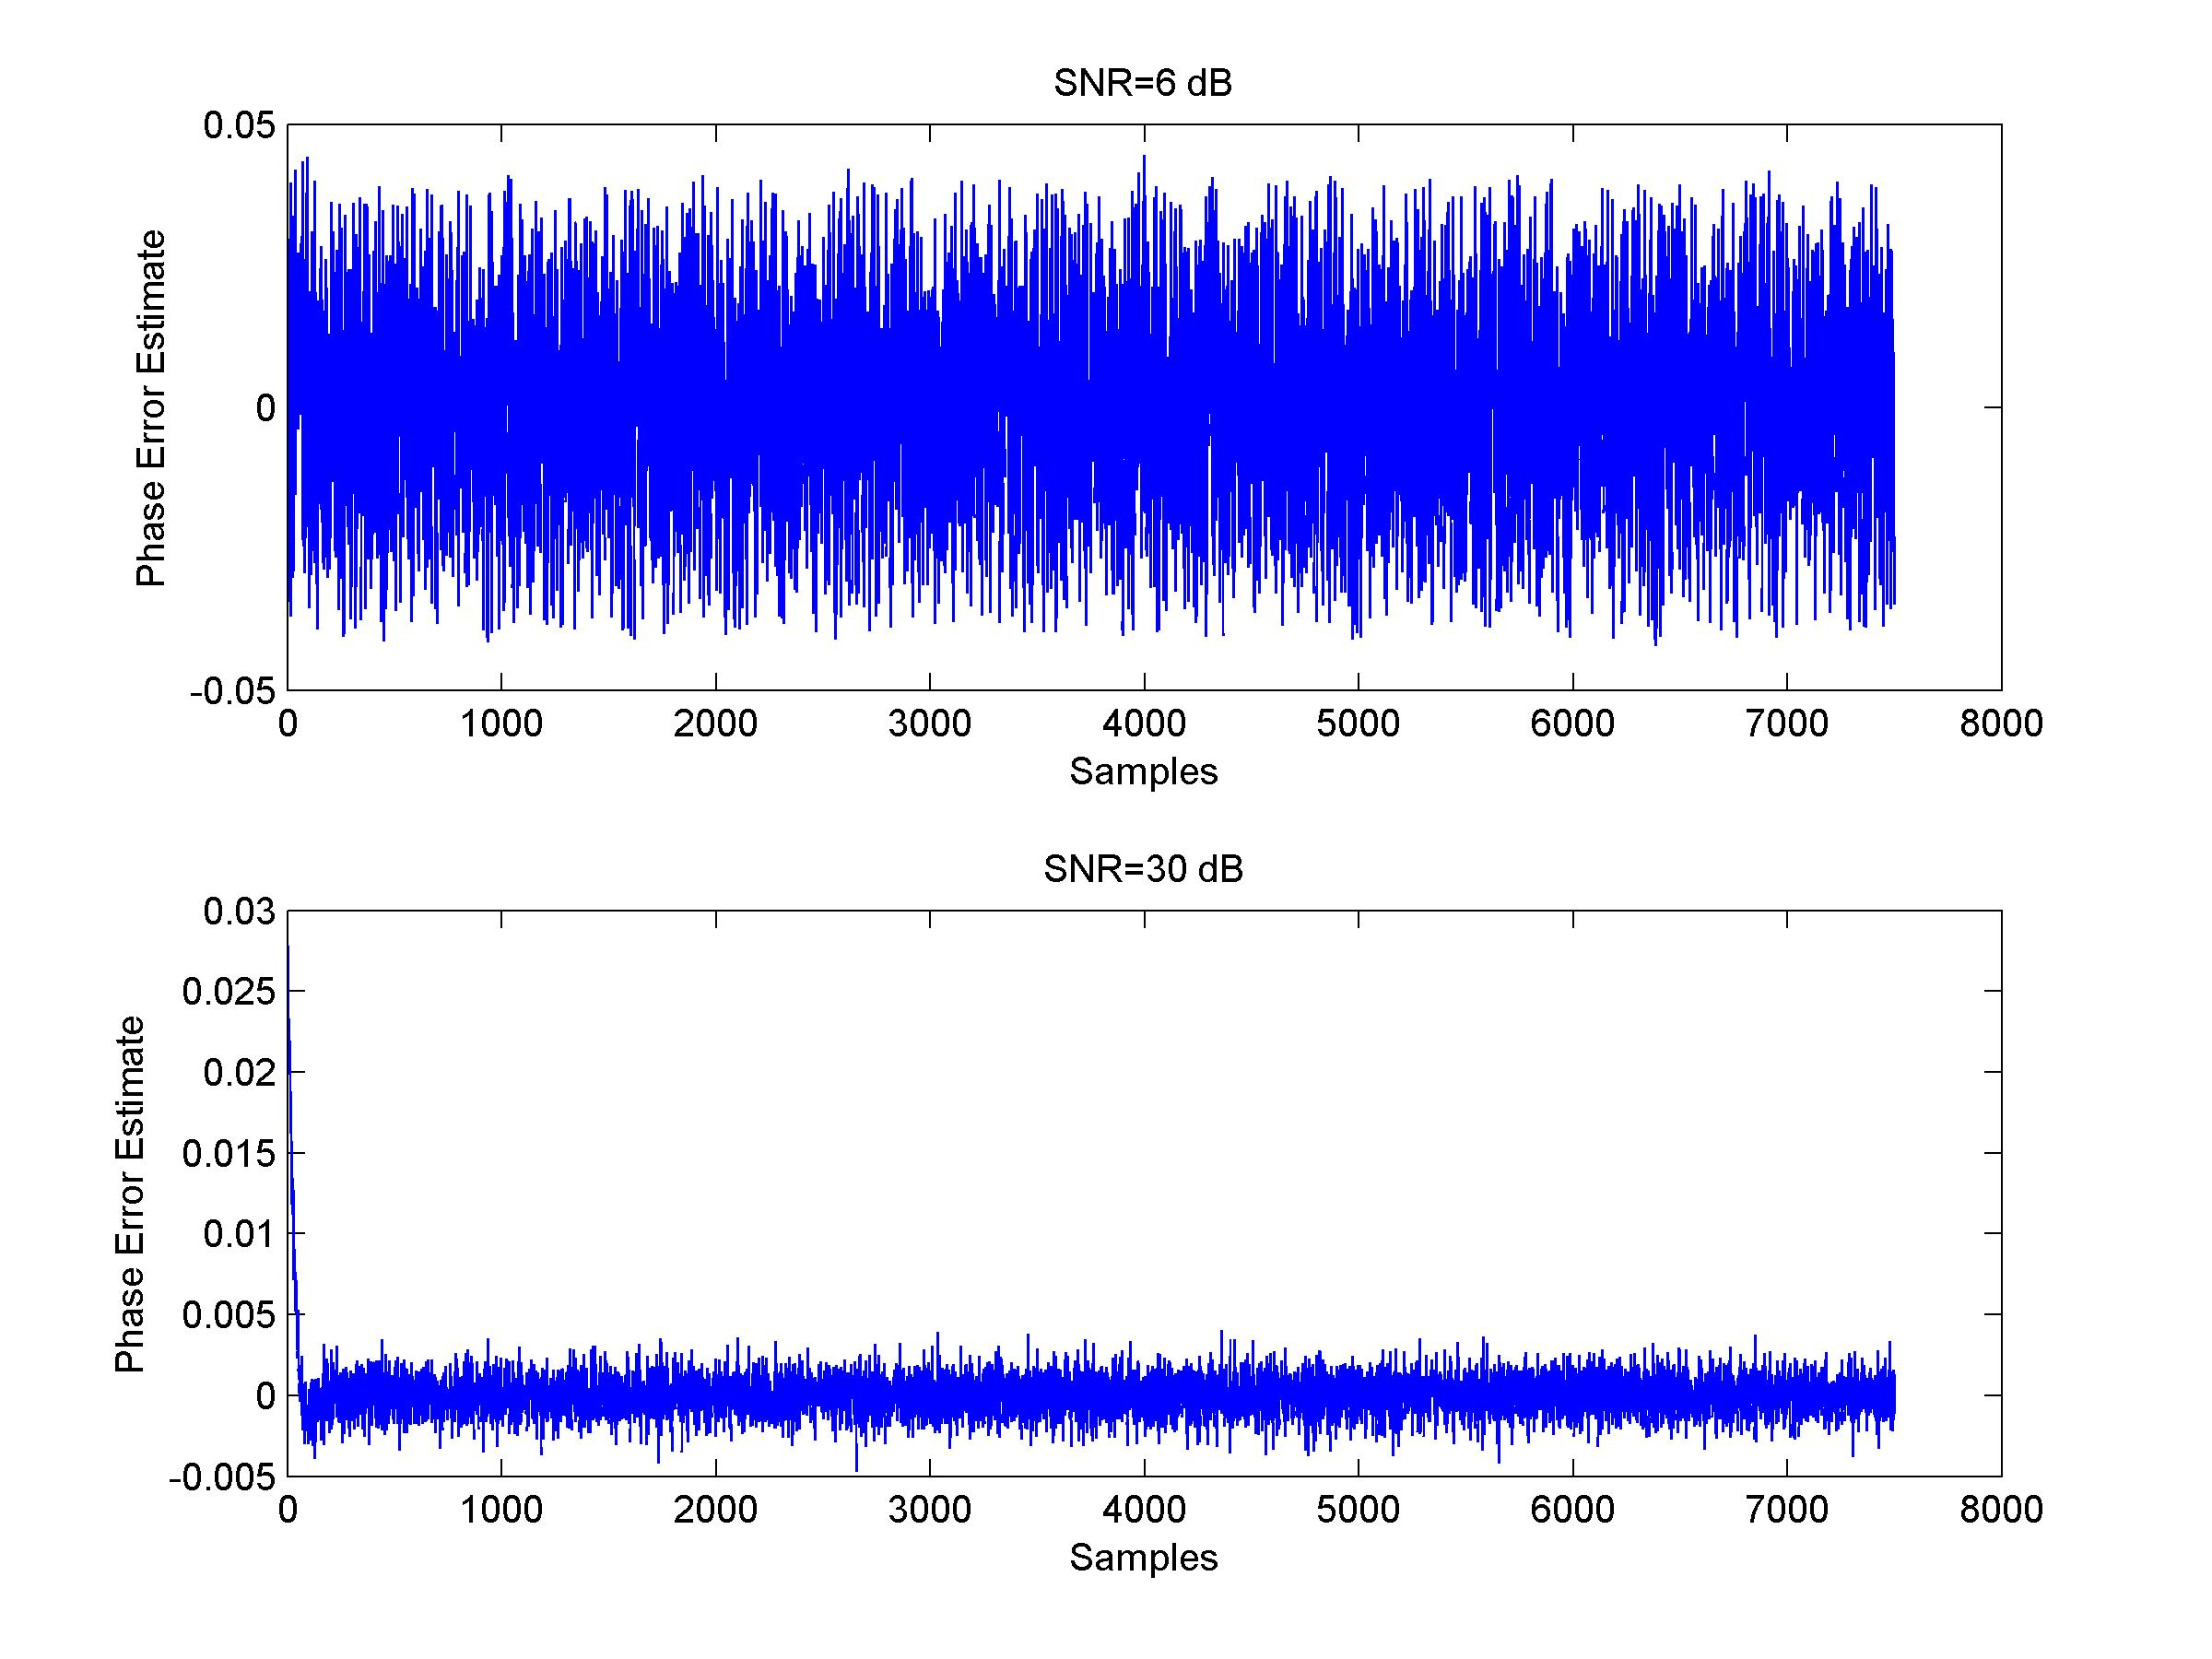
\includegraphics[width=0.5\textwidth]{qpLoopFilterpo_ddr1.jpg}
\caption{}
\end{figure}

\subsubsection{Transience of Carrier Recovery}
\begin{figure}[H]
\centering
\hspace*{-2cm}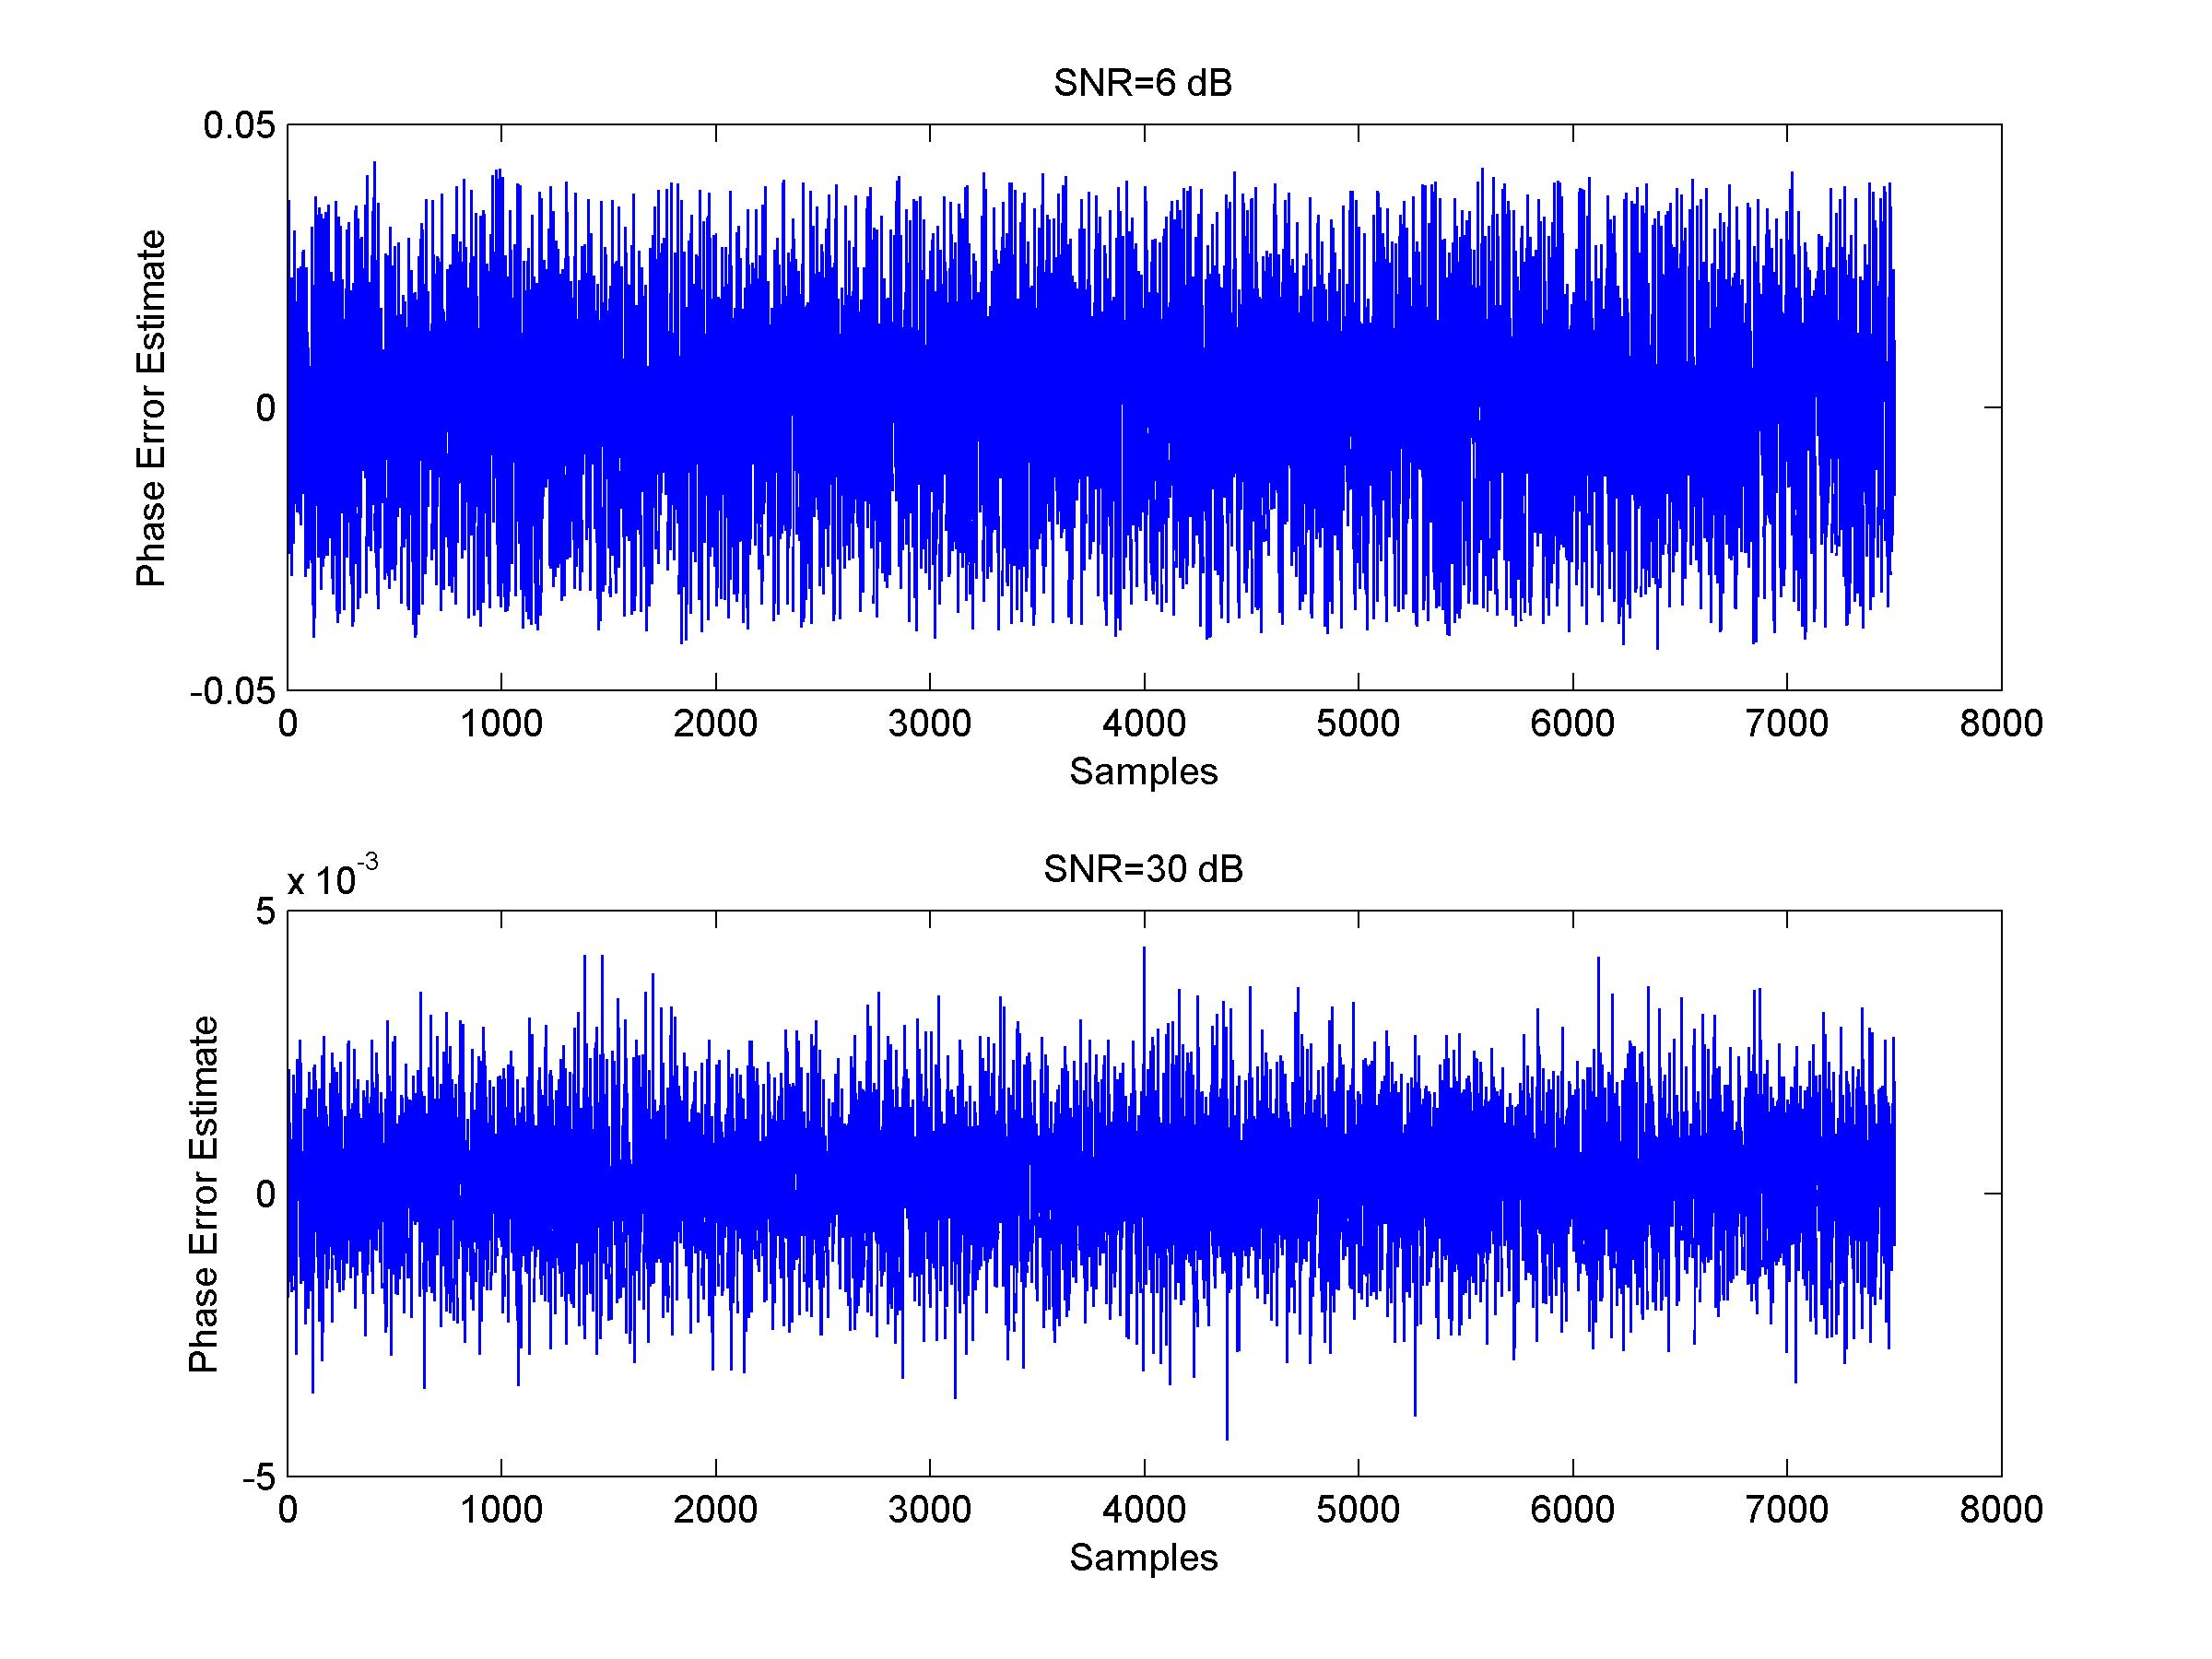
\includegraphics[width=0.5\textwidth]{qpLoopFilterfo_ddr1.jpg}
\caption{}
\end{figure}

\begin{figure}[H]
\centering
\hspace*{-2cm}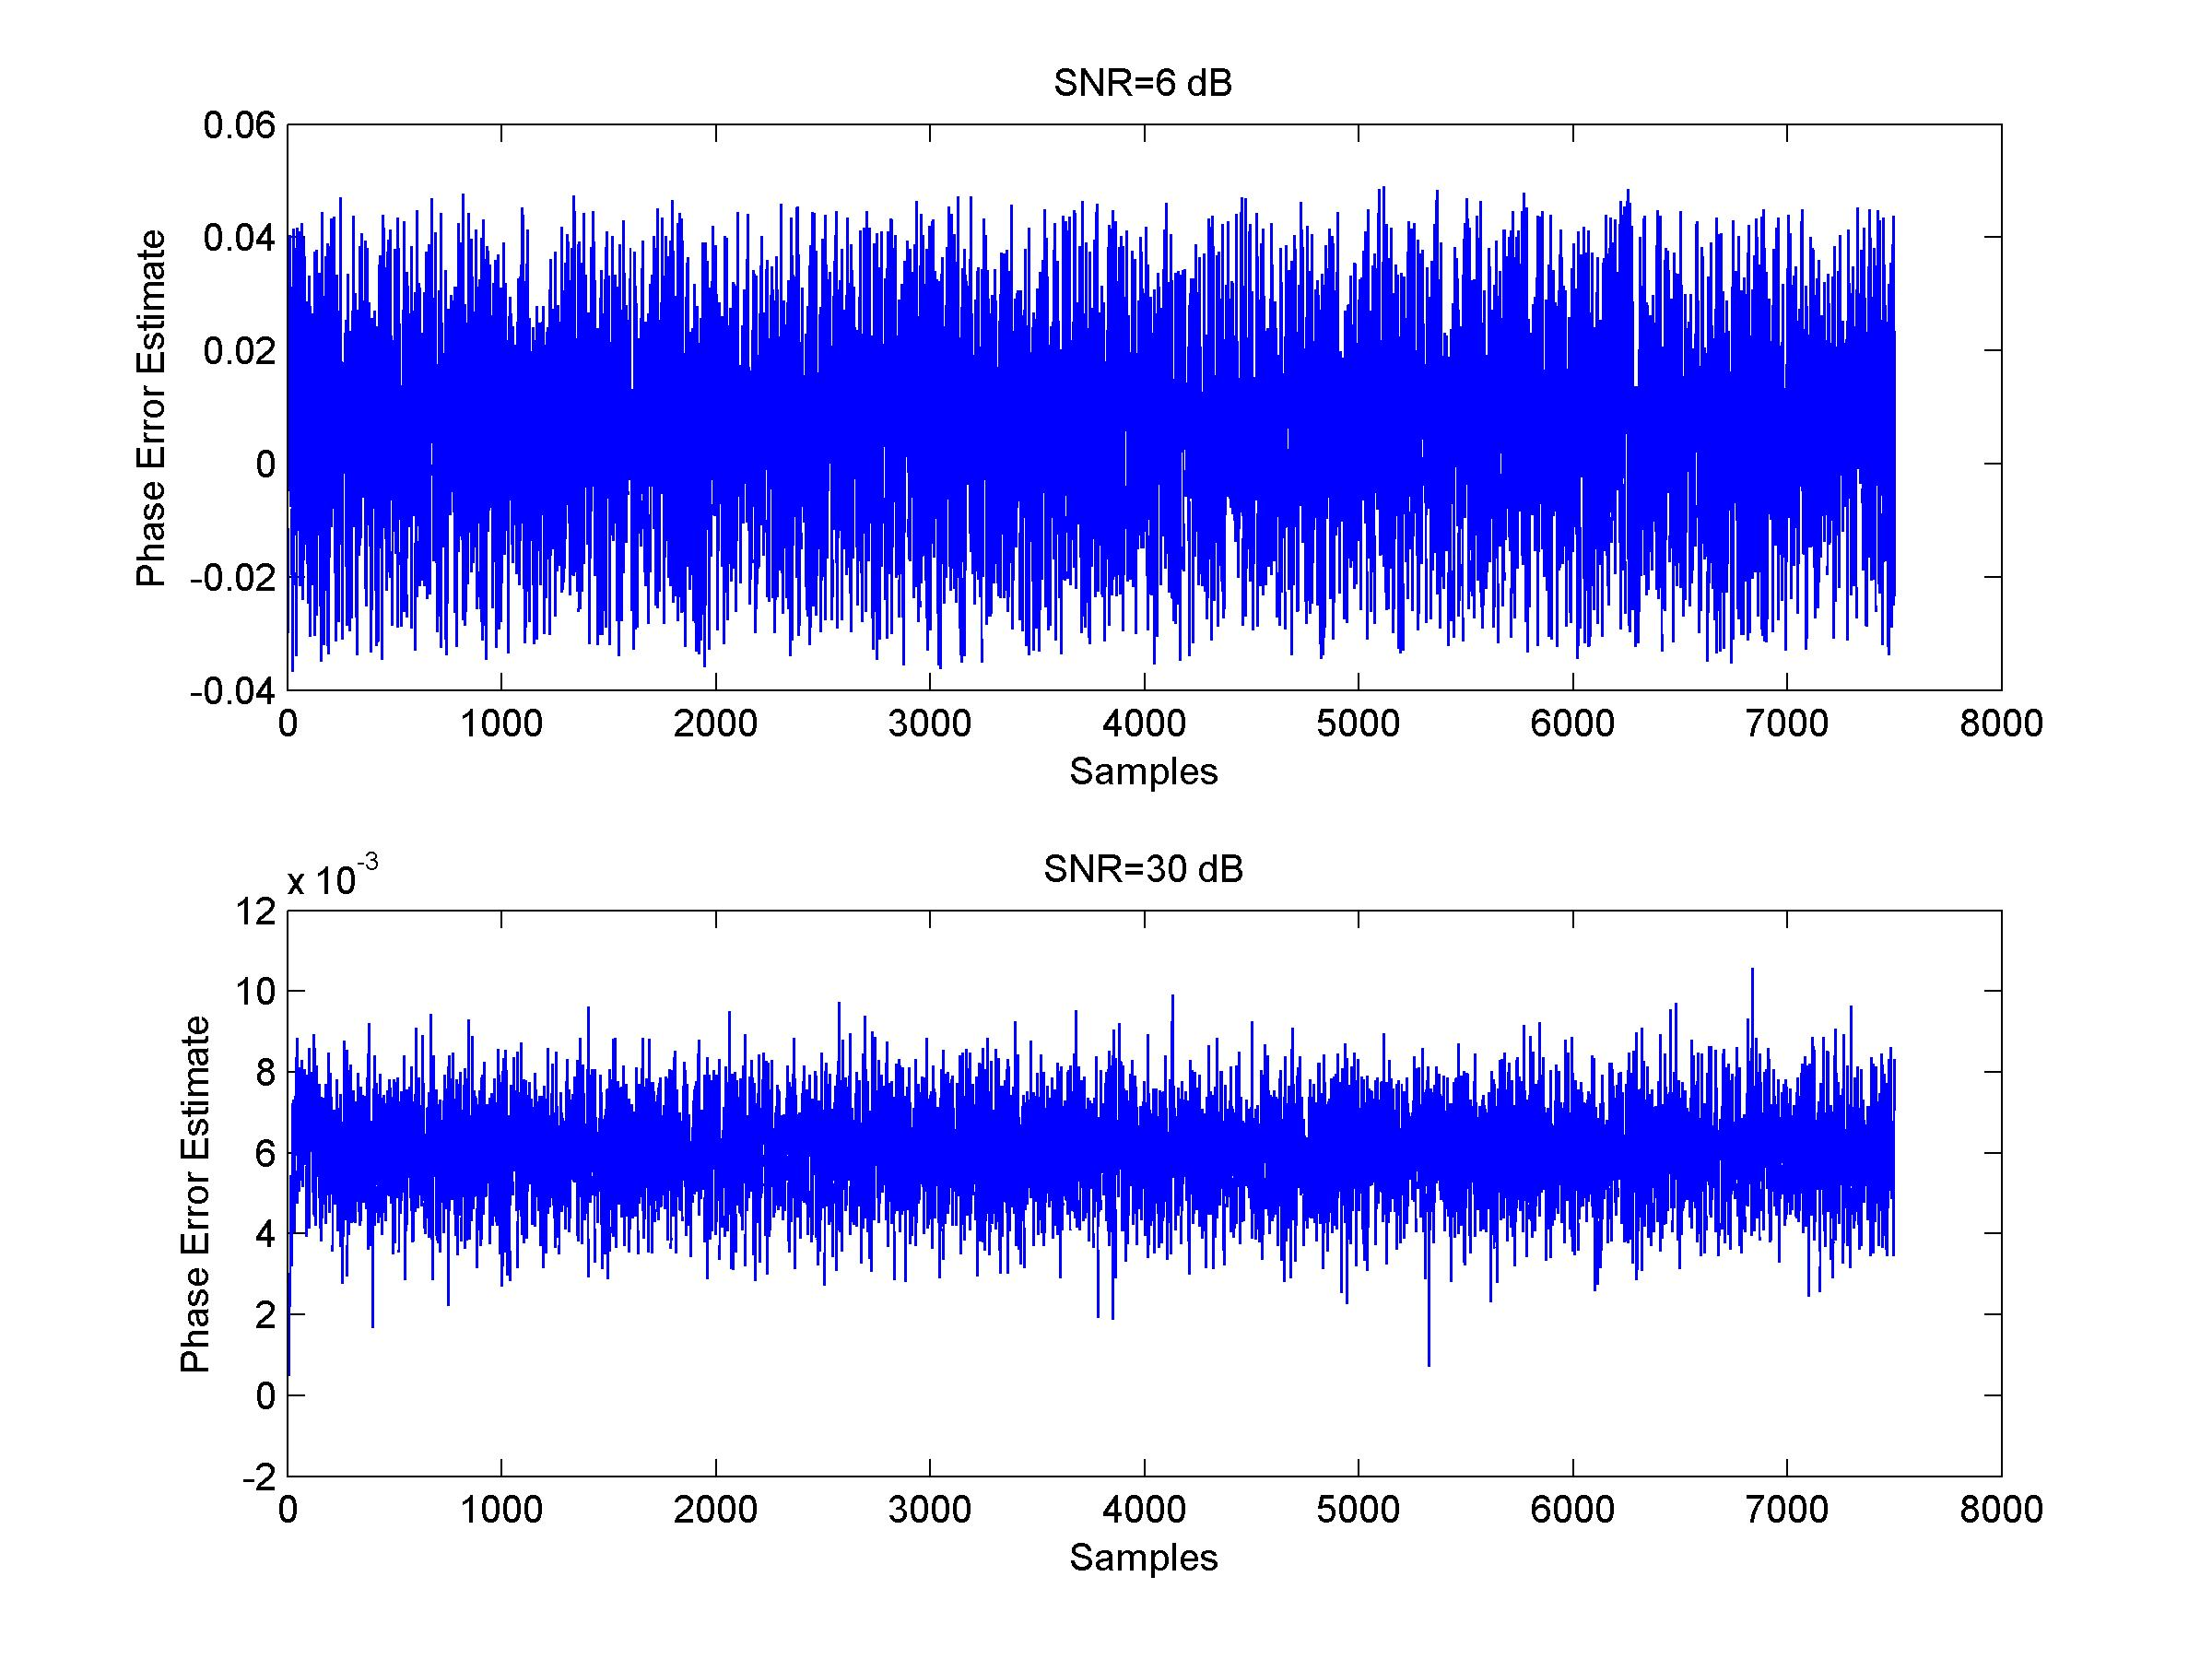
\includegraphics[width=0.5\textwidth]{qpLoopFilterfo_ddr2.jpg}
\caption{}
\end{figure}
\subsubsection{Constellation Plots  for Phase Recovery}
\begin{figure}[H]
\centering
\hspace*{-2cm}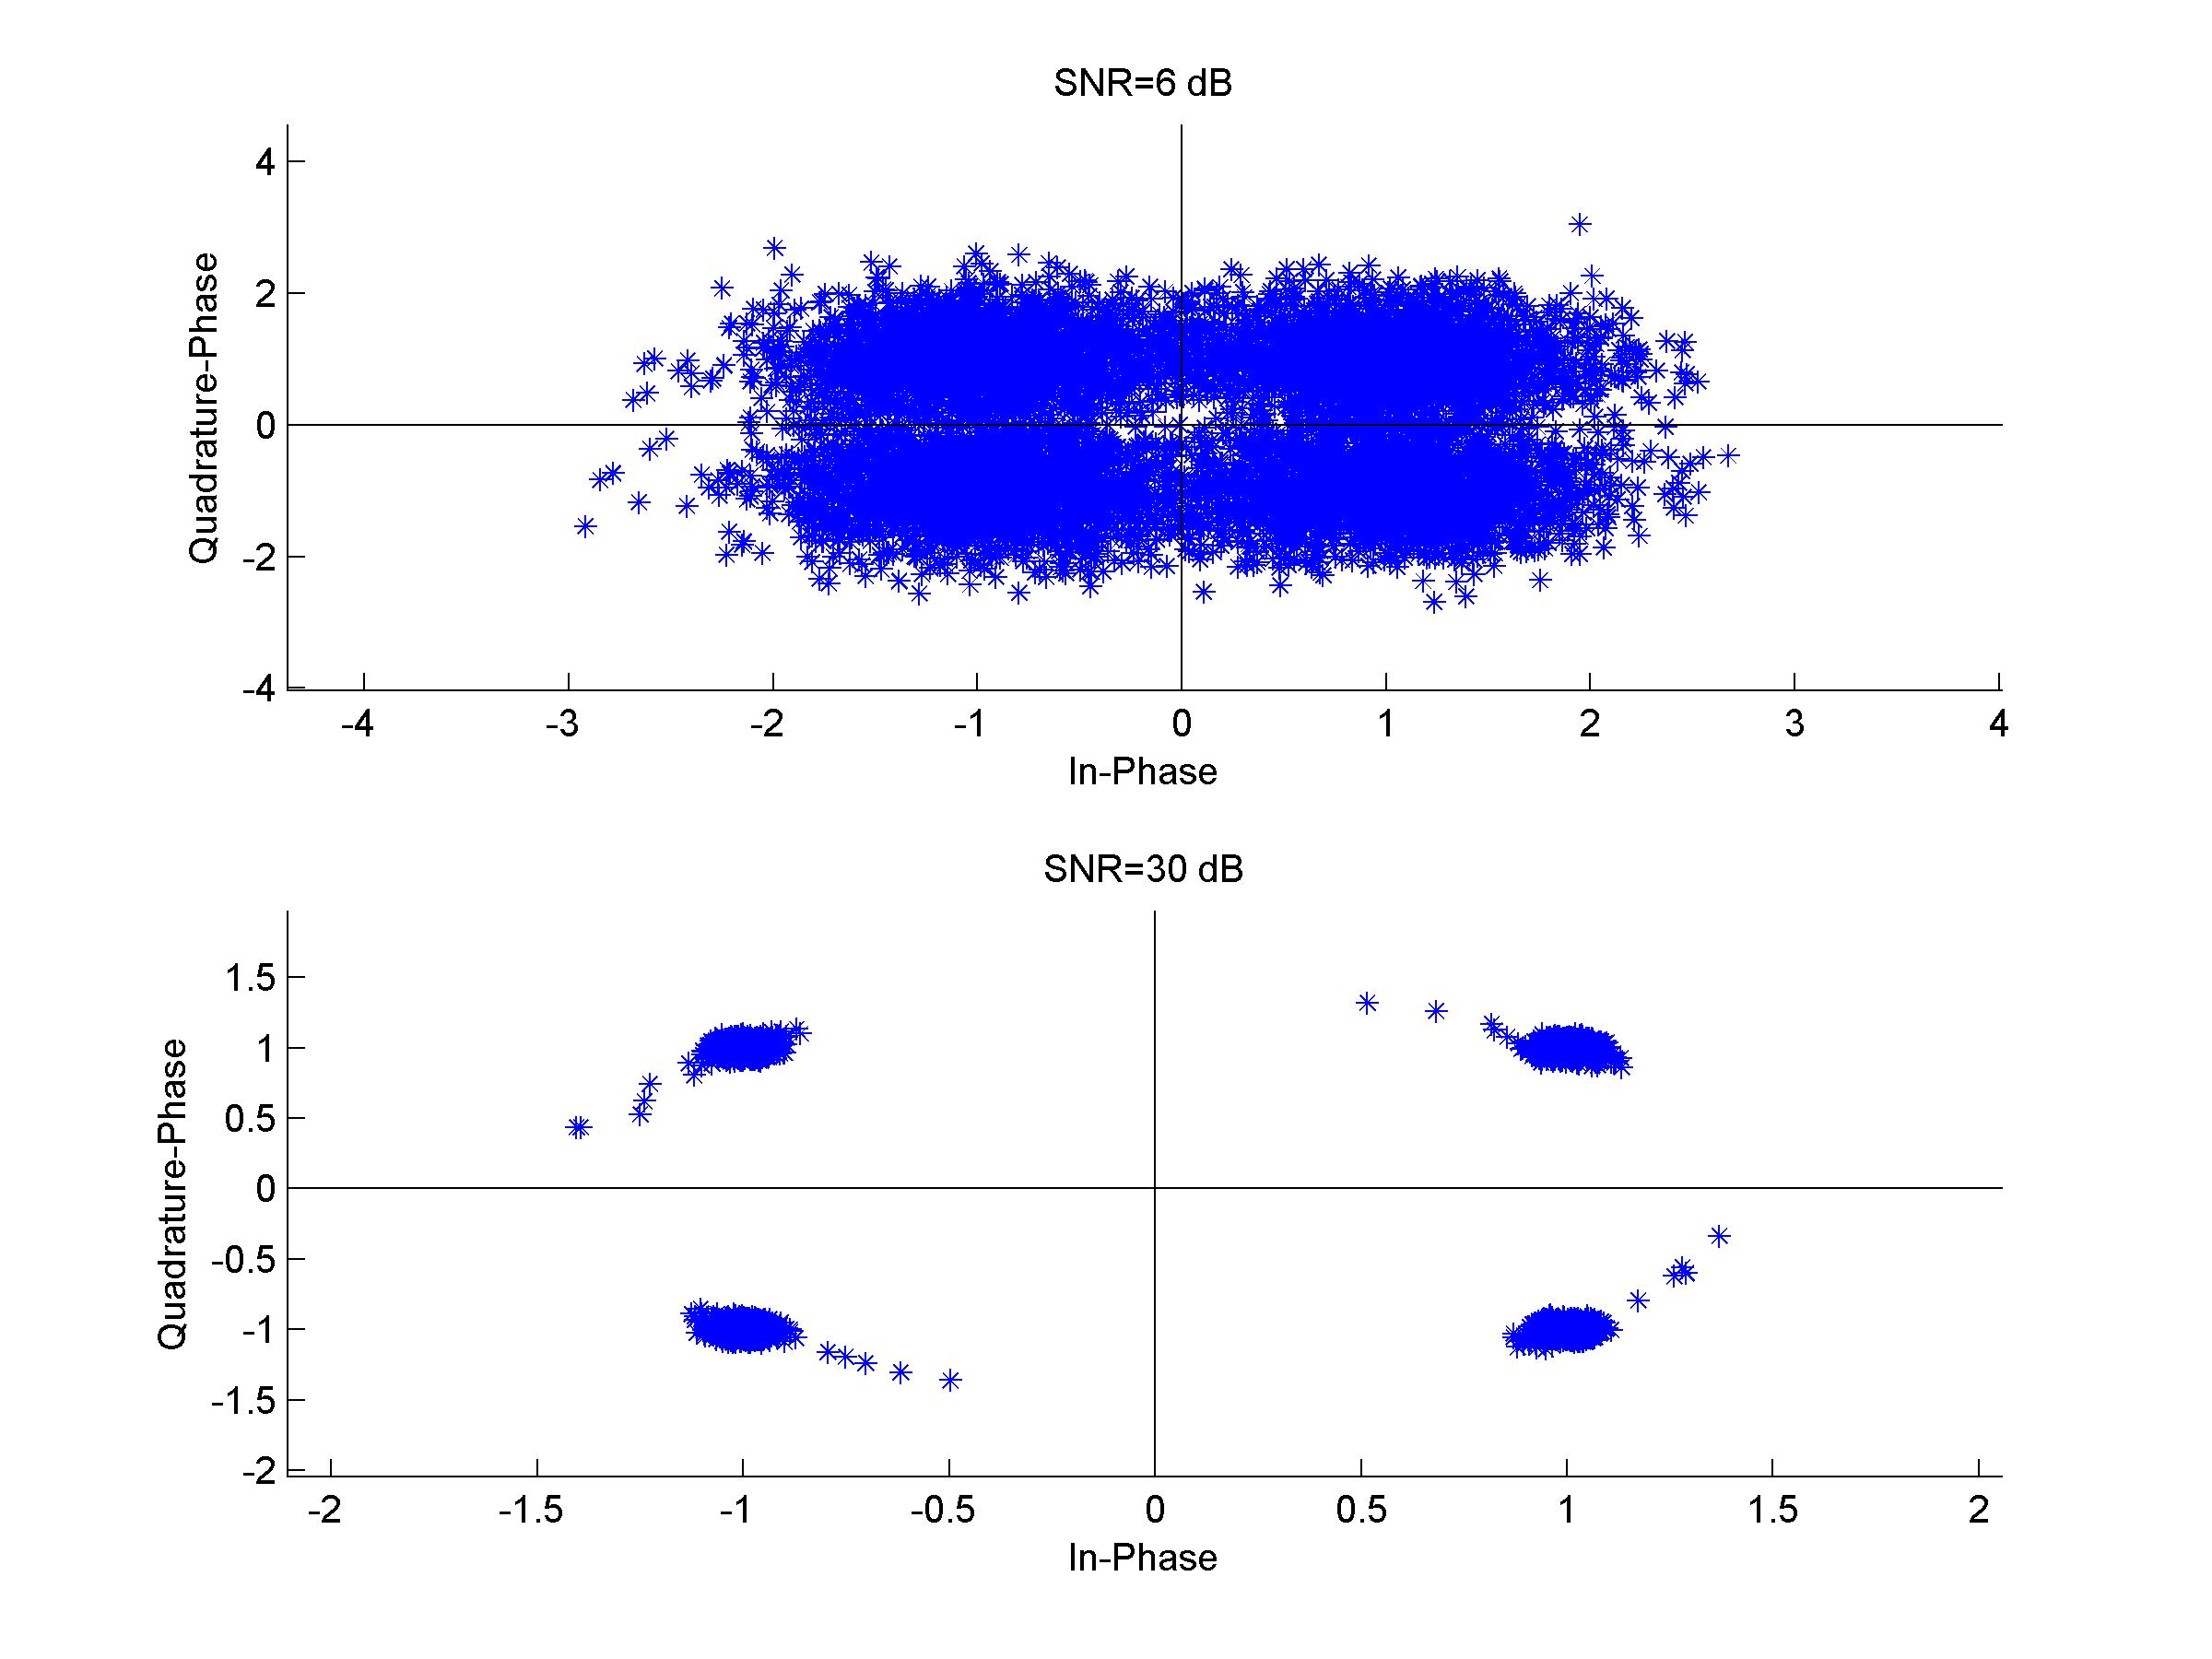
\includegraphics[width=0.5\textwidth]{qpConstpo_ddr1.jpg}
\caption{}
\end{figure}

\subsubsection{BER Plots for Carrier Recovery}
\begin{figure}[H]
\centering
\hspace*{-2cm}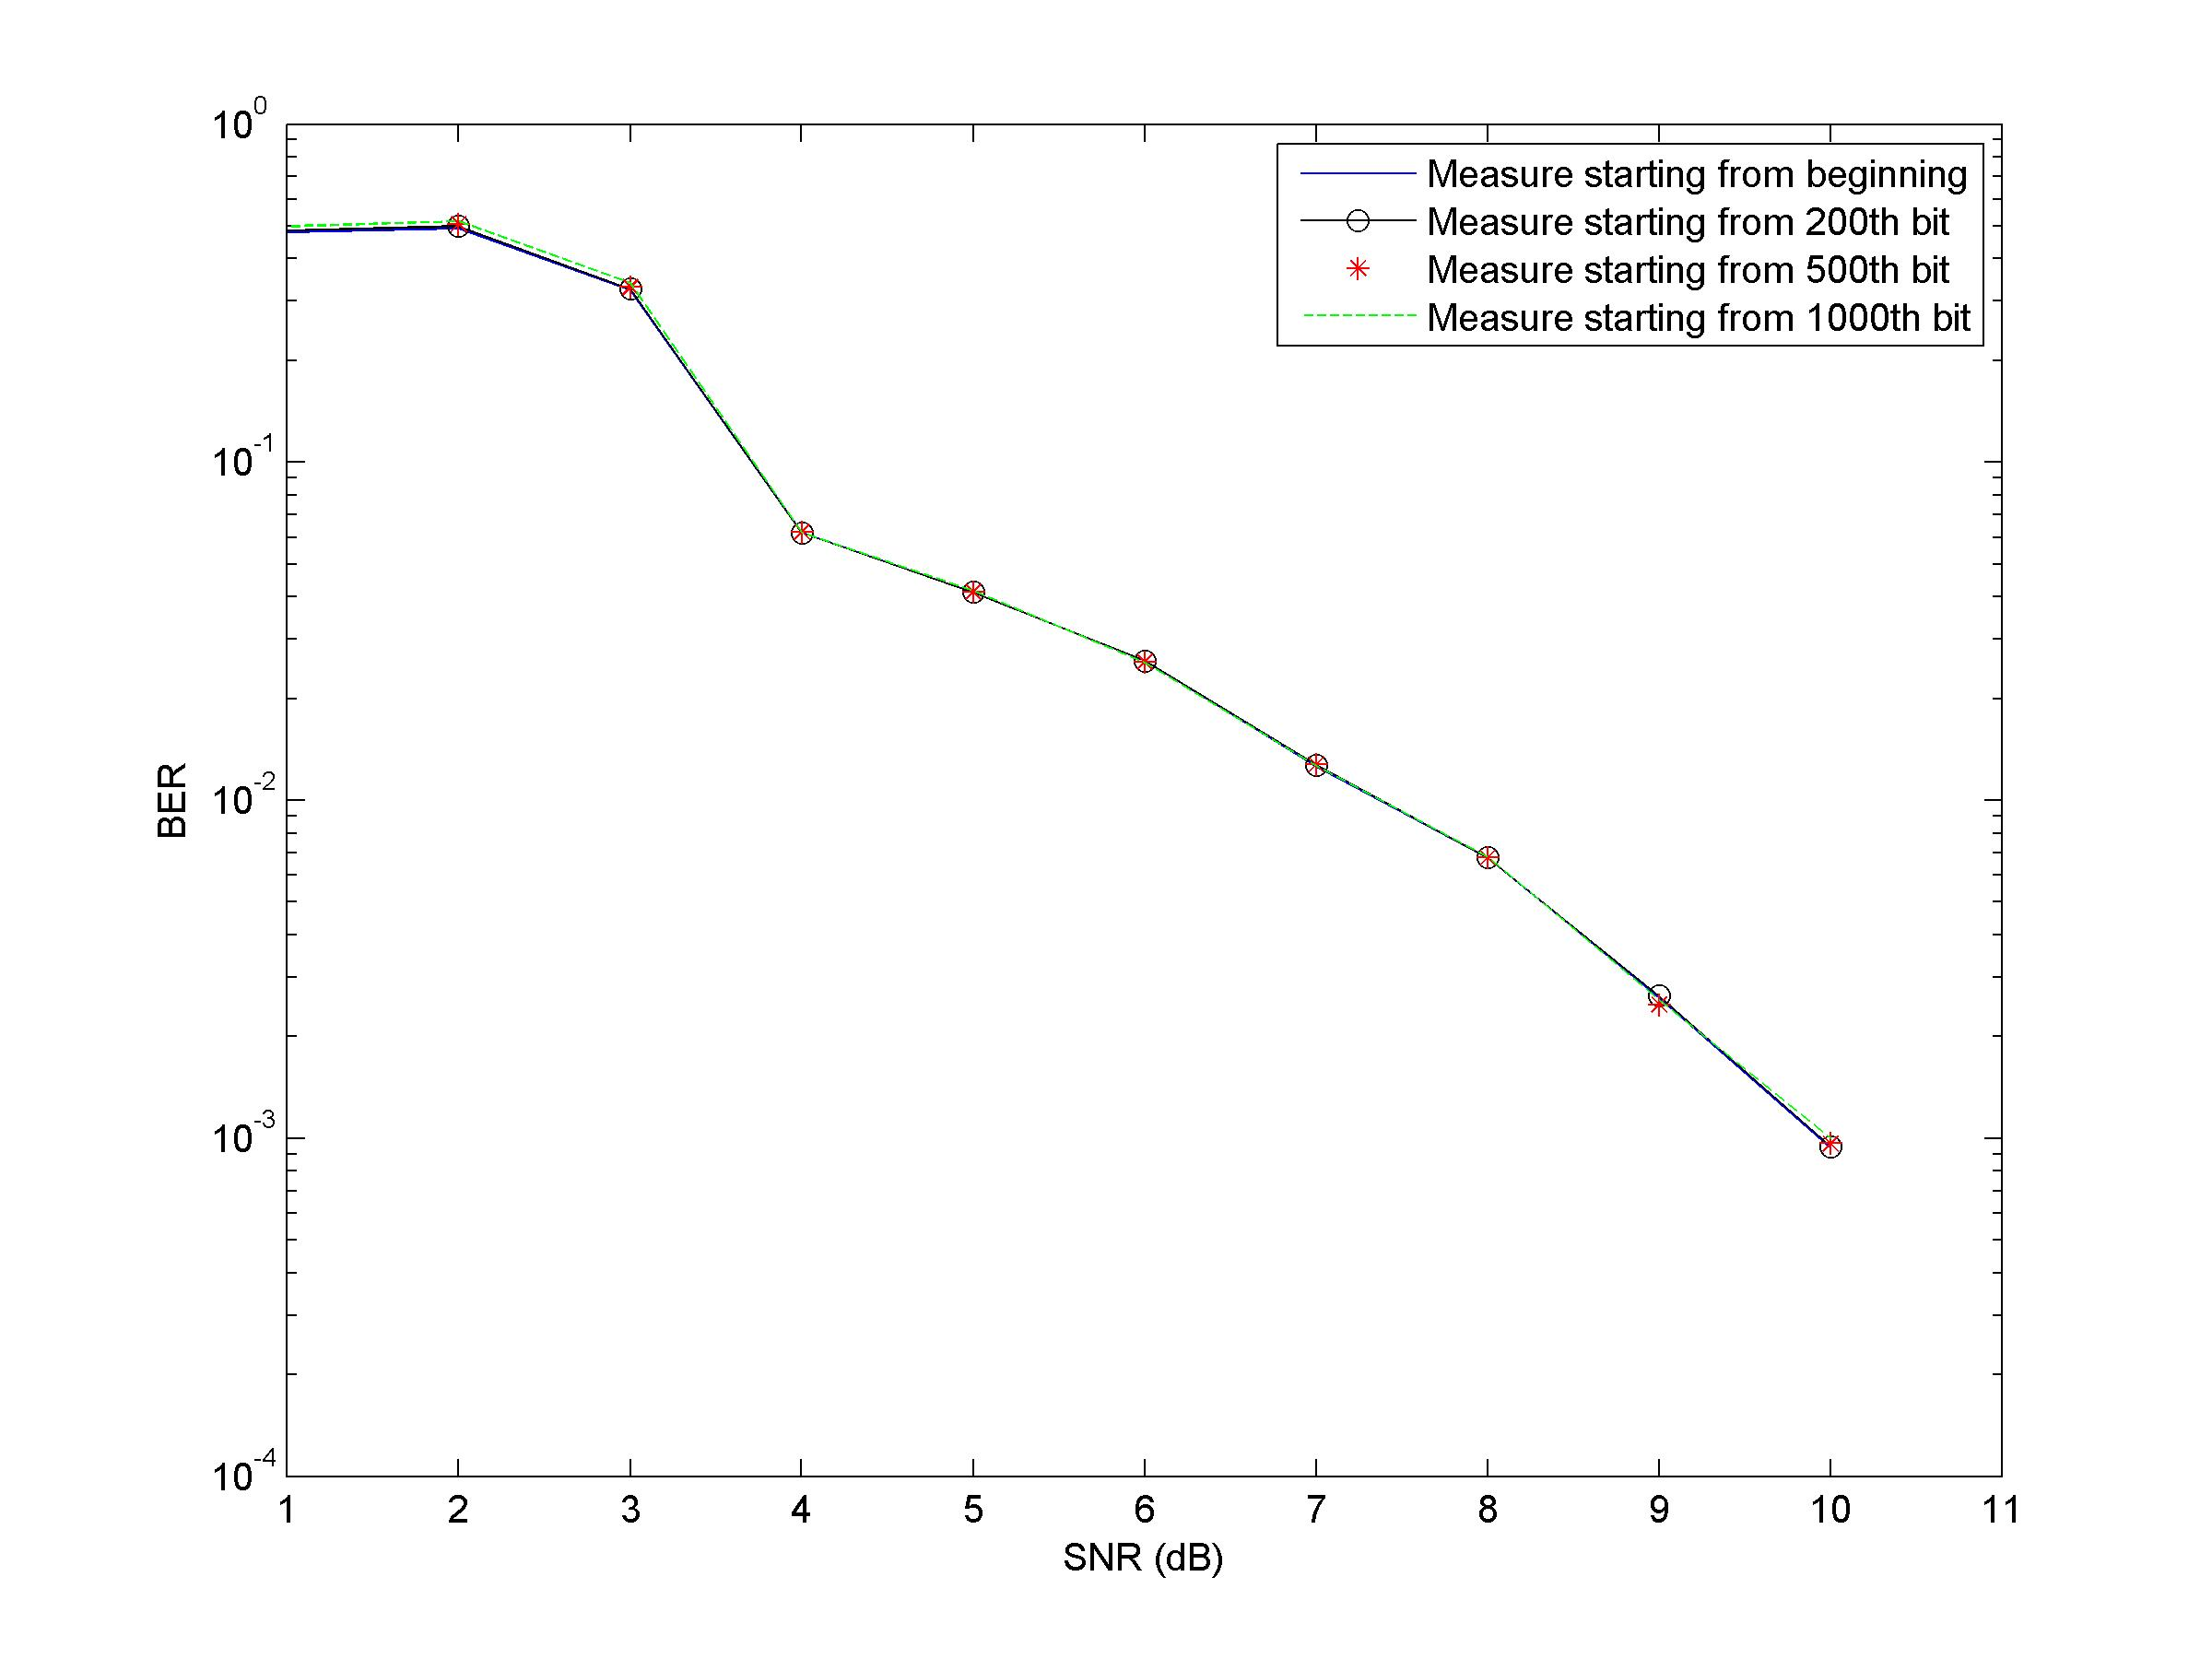
\includegraphics[width=0.5\textwidth]{qpBERfo_ddr1.jpg}
\caption{}
\end{figure}

\begin{figure}[H]
\centering
\hspace*{-2cm}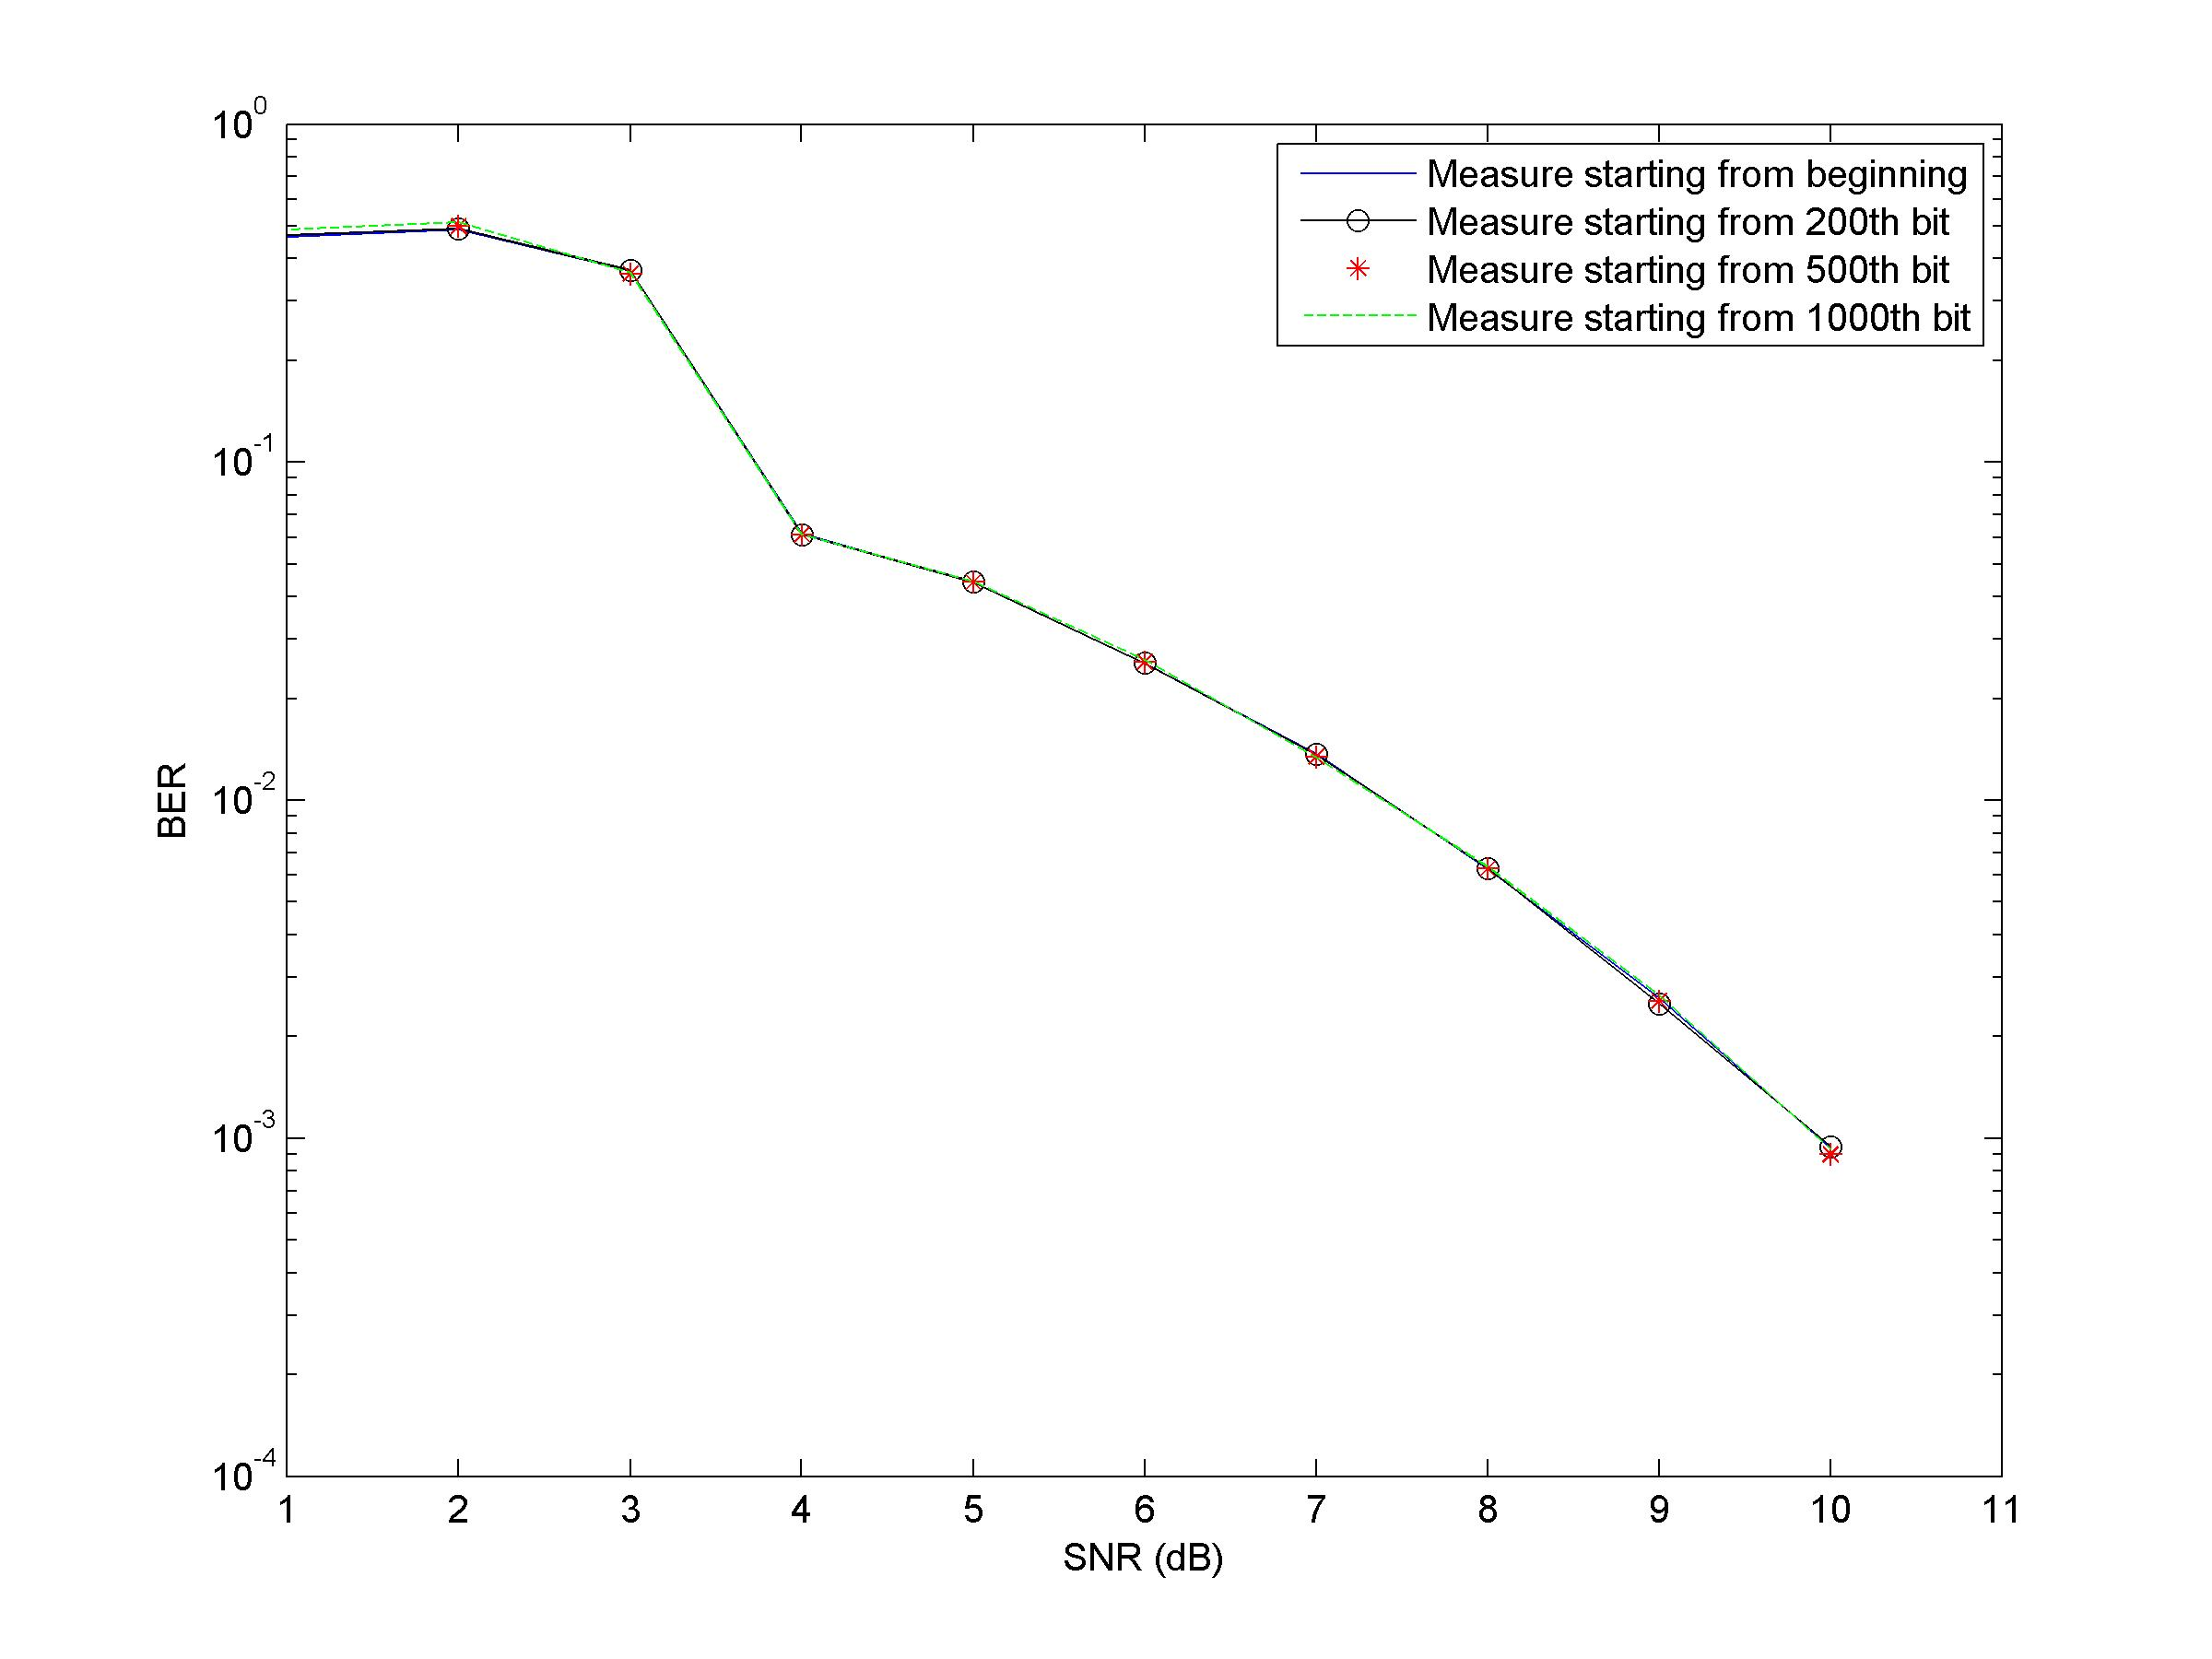
\includegraphics[width=0.5\textwidth]{qpBERfo_ddr2.jpg}
\caption{}
\end{figure}

\subsubsection{BER Plots for Phase Recovery}
\begin{figure}[H]
\centering
\hspace*{-2cm}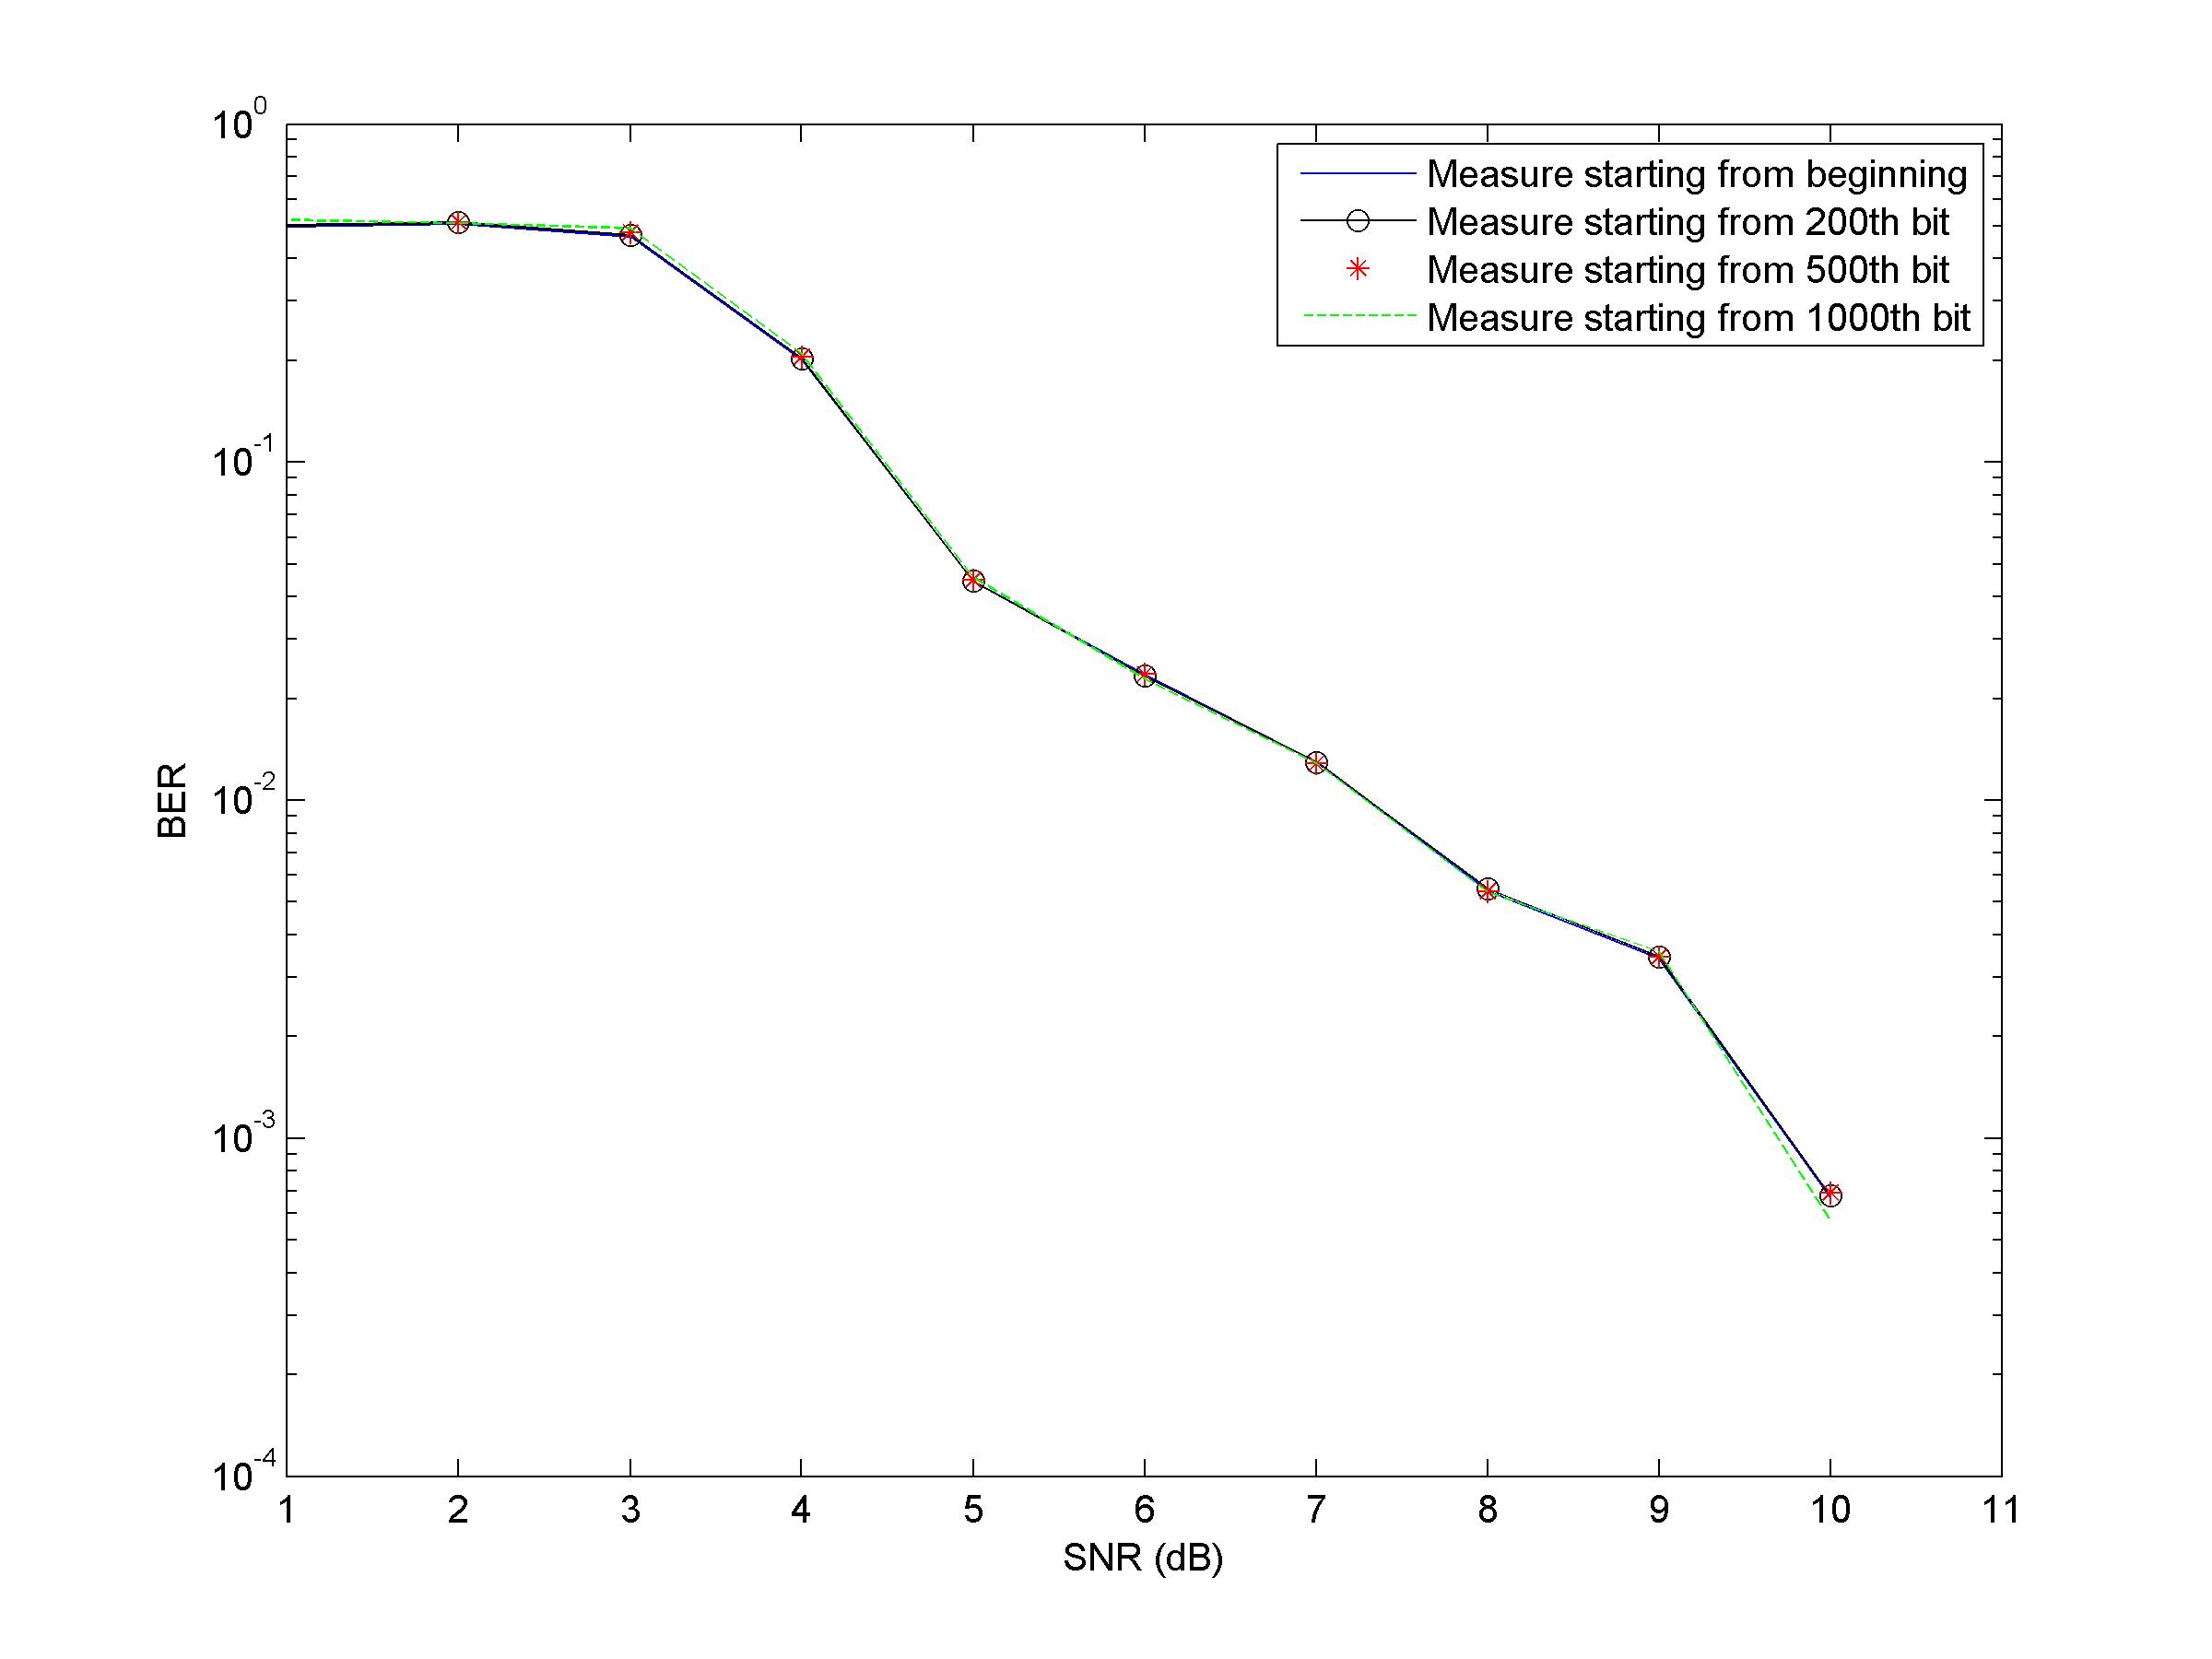
\includegraphics[width=0.5\textwidth]{qpBERpo_ddr1.jpg}
\caption{}
\end{figure}

\newpage
\section{Step 3 `S' Curves}
\label{sec:scurves}
To analyze the estimation, `S' curves graphically show how the estimation aligns with the actual error.  Figure~\ref{fig:scurvePhase} shows the phase estimate vs. phase for QPSK.   


\subsubsection{QPSK with Phase Offset}
\label{sec:s_phase}
%\begin{figure}[H]
%\centering
%\hspace*{-2cm}\includegraphics[width=0.4\textwidth]{scurvePhase.jpg}
%\caption{This plots the estimation versus actual phase error.  It is called an `S' curve because of its resemblance to the letter \label{fig:scurvePhase}
%\end{figure}

\subsubsection{QPSK with Frequency Offset}
\label{sec:s_freq}
%\begin{figure}[H]
%\centering
%\hspace*{-2cm}\includegraphics[width=0.4\textwidth]{scurveFreq.jpg}
%\caption{This plots the estimation frequency versus actual frequency error.  It is called an `S' curve because of its resemblance to the letter \label{fig:scurvePhase}
%\end{figure}


\newpage
\section{Conclusion}
\label{sec:conc}

\appendix
\newpage
\bibliographystyle{plain}
\bibliography{step3}
\newpage
%% the \\ insures the section title is centered below the phrase: Appendix B
%\section{Project Assignment}
%\label{app:assign}
%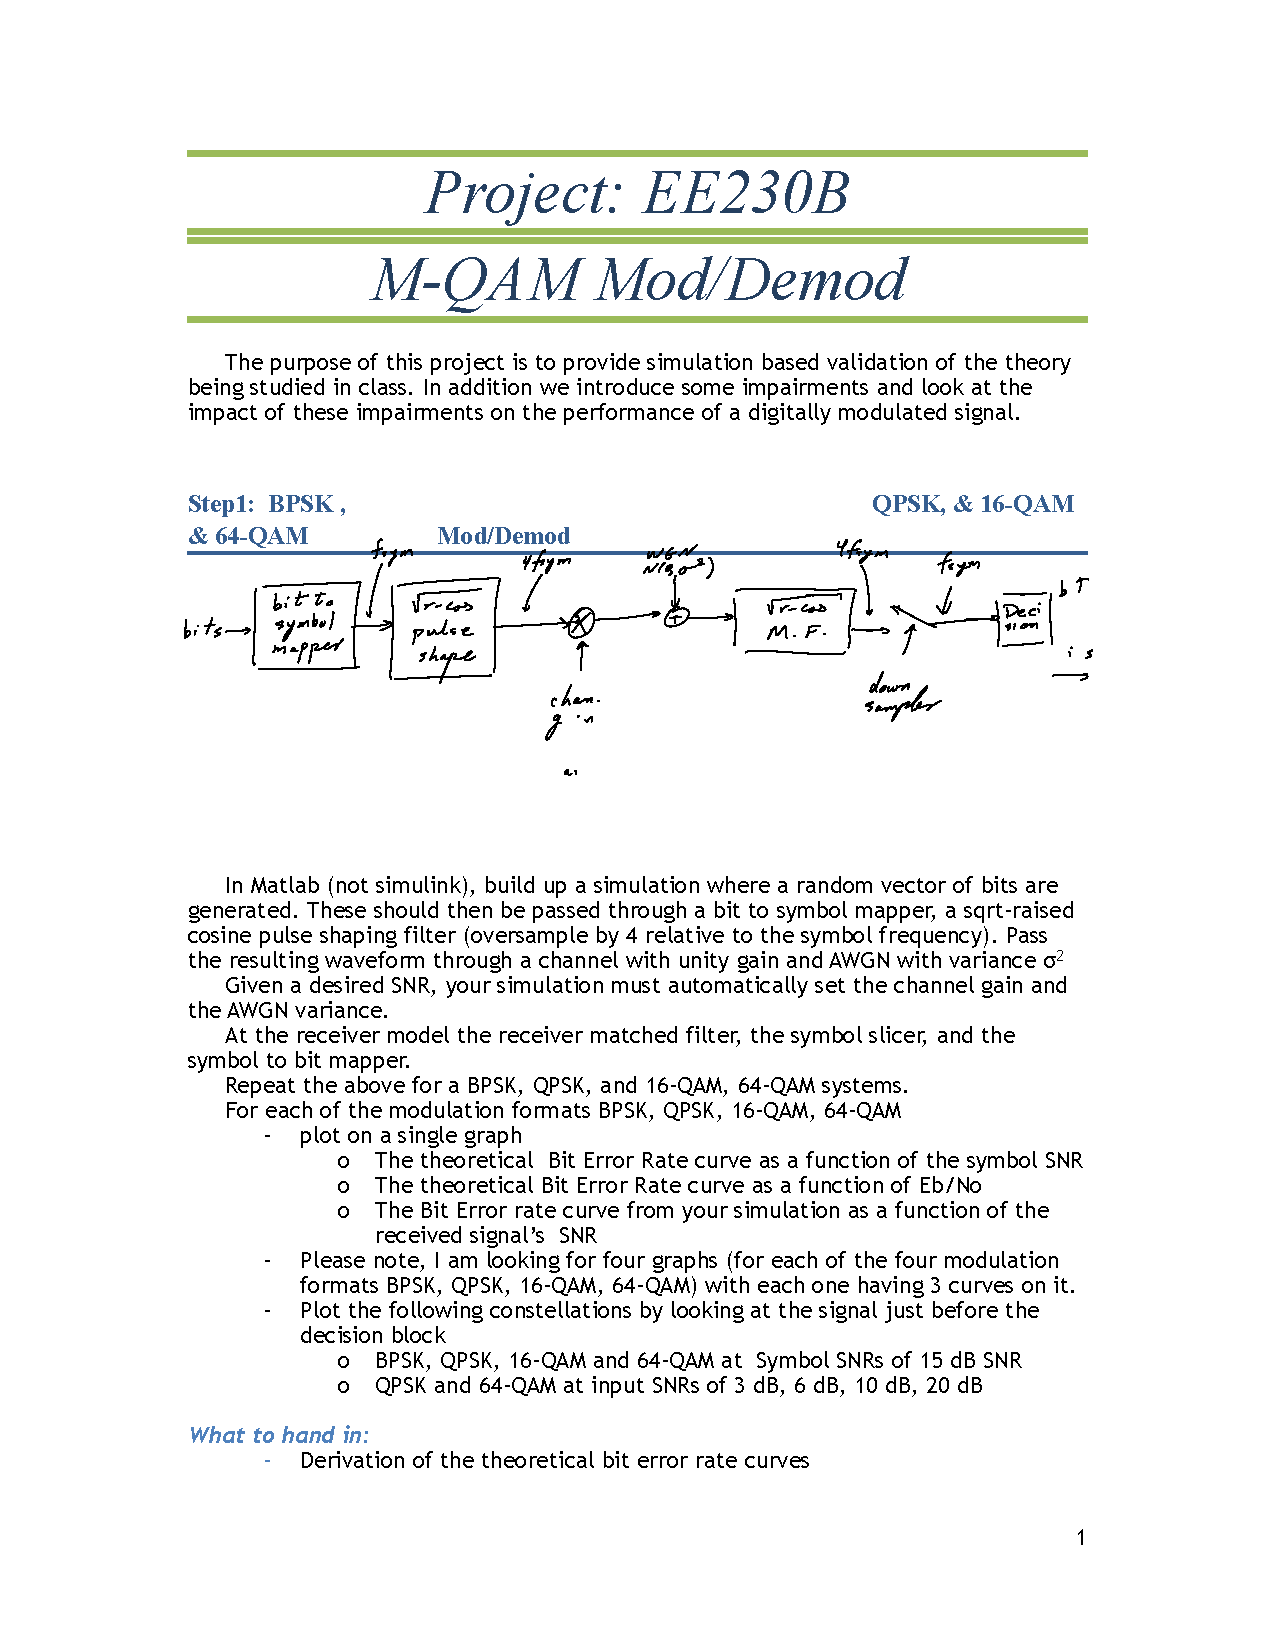
\includepdf[pages={1-5}]{project_overview.pdf}
%\cleardoublepage
%\newpage


\section{Random Bit Sequence Generator}
\label{app:random_bit_generator}
\lstinputlisting{random_bit_generator.m}

\section{Bit to Symbol Mappers}
\label{app:bittosym}
\subsection{BPSK Modulation }
\label{app:bpsk_mod}
% To convert program (e.g. C++ Fortran, Matlab, LaTeX) listings to a
% form easily includable in a LaTeX document
%
% type lgrind -s to see options
% lgrind -llatex -i sample-paper.tex > sampleinputtex
% creates a file sampleinput.tex which can then be included into this
% document simply by uncommenting the next line
%\lgrindfile{testinput.tex}

\lstinputlisting{bpsk_mod.m}

\subsection{QPSK Modulation}
\label{app:qpsk_mod}
\lstinputlisting{qpsk_mod.m}

\subsection{16-QAM Modulation}
\label{app:qam_16_mod}

\lstinputlisting{QAM_16_mod.m}

\subsection{64-QAM Modulation }
\label{app:qam_64_mod}
\lstinputlisting{QAM_64_mod.m}

\newpage
\section{Square Root Raised Cosine Filter}
\label{app:sqrt_raised_cosine}
\lstinputlisting{sqrt_raised_cosine.m}


\section{Up Sampler}
\label{app:impulse_train}
\lstinputlisting{impulse_train.m}

\section{Additive Gaussian White Noise Channel}
\label{app:awgn_channel}
\lstinputlisting{awgn_complex_channel.m}

\newpage
\section{Sampler}
\label{app:sampler}
\lstinputlisting{sampler.m}


\section{Decision Blocks}
\label{app:dblocks}
\subsection{BPSK Demodulation}
\label{app:bpsk_demod}
\lstinputlisting{bpsk_demod.m}

\newpage
\subsection{QPSK Demodulation}
\label{app:qpsk_demod}
\lstinputlisting{qpsk_demod.m}

\subsection{16-QAM Demodulation}
\label{app:qam_16_demod}
\lstinputlisting{QAM_16_demod.m}

\newpage
\subsection{64-QAM Demodulation}
\label{app:qam_64_demod}
\lstinputlisting{QAM_64_demod.m}

\newpage
\section{Offsets}
\label{app:offsets}
\subsection{Carrier Phase Offset}
\label{app:phase_offset}
\lstinputlisting{phase_offset.m}

\newpage
\subsection{Carrier Frequency Offset}
\label{app:freq_offset}
\lstinputlisting{freq_offset.m}


\end{document}